% !TEX encoding = UTF-8 Unicode

\documentclass[a4paper,14pt,oneside,italian]{book}
\usepackage[left = 3cm, right = 3cm]{geometry}
\usepackage{babel}
\usepackage{graphicx}
\usepackage{amsthm,amssymb}
\usepackage[makeroom]{cancel}
\usepackage[pdfencoding=auto]{hyperref}
\usepackage{mathtools,thmtools}
\usepackage{cleveref}
\usepackage{pgfplots}
\usepgfplotslibrary{fillbetween}
\usepackage{accents}
\usepackage{xparse}
\usepackage{hyperref}
\usepackage{etoolbox}

\counterwithout{section}{chapter}

\newtheorem{theorem}{Teorema}[section]
\newtheorem{definition}[theorem]{Definizione}
\newtheorem{proposition}[theorem]{Proposizione}
\newtheorem{observation}[theorem]{Osservazione}
\newtheorem{corollary}[theorem]{Corollario}
\newtheorem{lemma}[theorem]{Lemma}
\newtheorem{example}[theorem]{Esempio}
\newtheorem{exercise}[theorem]{Esercizio}
\newtheoremstyle{note}
  {} % space above note
  {} % space below note
  {\normalfont\small\addtolength{\leftskip}{1em}} % body font and position
  { } % space to indent the head
  {\bfseries} % head font
  {.} % punctuation between head and body
  { } % space after theorem head; " " = normal interword space
  { } % Manually specify head
\theoremstyle{note}
\newtheorem*{note}{Nota}

\newenvironment{solution}
  {\renewcommand\qedsymbol{$\blacksquare$}\begin{proof}[Soluzione]}
  {\end{proof}}

\begin{document}
\newcommand{\norm}[1] {\left\|#1\right\|}
\newcommand{\abs}[1] {\left|#1\right|}
\newcommand{\brackets}[1] {\left\{#1\right\}}

\newcommand{\R}{\mathbb{R}}
\newcommand{\N}{\mathbb{N}}
\newcommand{\bbset}[1] {\mathbb{#1}}
\newcommand{\bbsetn}[2] {\mathbb{#1}^{#2}}

\newcommand{\integrald}[1]{\,\mathrm{d}{#1}}

\newcommand{\bfset}[1] {\mathbf{#1}}

\newcommand{\cntclass}[1] {\mathbf{C^{#1}}} % Command for continuity classes

\newcommand{\realintervalopen}[2] {\left]#1,#2\right[}
\newcommand{\realintervalclose}[2] {\left[#1,#2\right]}
\newcommand{\realintervalclop}[2] {\left[#1,#2\right[}
\newcommand{\realintervalopcl}[2] {\left]#1,#2\right]}
\newcommand{\realfunction}[3]{ #1:#2\to#3}
\newcommand{\trigonpol}[3] {\frac{a_0}{2}+\sum\limits_{#1=#2}^{#3}a_{#1}cos(#1x)+b_{#1}sin(#1x)}

\newcommand{\dinfty}[2]{d_\infty\left(#1,#2\right)}
\newcommand{\ddinfty}[3]{\sup\limits_{x\in#3}{\abs{f-g}}}
\newcommand{\sse}{\Leftrightarrow}
\newcommand{\bydef}{\rightleftharpoons}

\newcommand{\rvect}[1]{\begin{bmatrix} #1 \end{bmatrix}}

\newcommand{\circdot}[1]{\accentset{\circ}{#1}}

% Append the following to an equation in align* blocks to allow tagging single eq.
\newcommand*{\tageq}{\refstepcounter{equation}\tag{\theequation}}
% Use the following to align vertically an equation in a align block without actually having the equals sign aligned
% Example:
%   5^2+3 =
%   = 25+3
%   = 28
\newcommand{\noaligneq}[1]{\noalign{\centering #1}}

\newcommand*{\fullref}[1]{\hyperref[{#1}]{\autoref*{#1} (\nameref*{#1})}} % To reference stuff with its name appended

\DeclareDocumentCommand{\funcdef}{m m o m o s o}{
  % This command allows formal function definition and require xparse
  % Taken from https://tex.stackexchange.com/questions/149705/defining-a-macro-with-three-optional-arguments-in-the-form-newmacroabcd
  \begin{array}{r@{\ }c@{\,}c@{\,}l}
    #1:
  & \IfNoValueTF{#3}{#4}{#3}
  & \to & #4 \\
  & #2
  & \mapsto
  & \IfNoValueTF{#5}{#1(#2)}{#5}
    \IfNoValueTF{#7}{}{\mathrel{:=}#7}
  \end{array}
}

\author{Mauro Conte, Federico Cerutti}
\title{Appunti di Analisi 2}
\date{Febbraio 2019}

\frontmatter
\maketitle
\tableofcontents

\mainmatter
\part{Spazi Metrici}
\chapter{Spazi Metrici}

\section{Preliminari}
\definition
Si dice spazio metrico un insieme X non vuoto in cui sia definita una
distanza(metrica), vale a dire una funzione $d: X \times X \rightarrow \R$ con le proprietà:
\begin{enumerate}
	\item $d(x,y)\ge0 \quad \forall x,y \in X$
	\item $d(x,y)=0\Leftrightarrow x=0 \quad \forall x,y \in X$
	\item $d(x,y)=d(y,x) \quad \forall x,y \in X$ simmetria
	\item $d(x,y)\le d(x,z)+d(z,y) \quad \forall x,y,z\in X$ disuguaglianza triangolare 
\end{enumerate}

\example
$$X=\bbsetn{R}{2},\quad d((x_1,y_1),(X_2,y_2))=\sqrt{(x_2-x_1)^2+(y_2-y_1)^2}$$
si dimostra che la funzione così definita è una distanza:
\begin{enumerate}
	\item $d(x_1,x_2)\ge 0$, è verificata poiché l'argomento della radice è sempre positivo o al più nullo essendo una somma di quadrati, e la radice mantiene le quantità positive.
	\item $d((x_1,y_1),(x_2,y_2))=0\Leftrightarrow \sqrt{(x_2-x_1)^2+(y_2-y_1)^2}=0$\\
	$\Leftrightarrow (x_2-x_1)^2+(y_2-y_1)^2=0 $
	$\Leftrightarrow \left\{\begin{matrix}
	(x_2-x_1)^2=0\\
	(y_2-y_1)^2=0\\
	\end{matrix}\right.\Leftrightarrow
	\left\{\begin{matrix}
	x_2=x_1\\
	y_2=y_1\\
	\end{matrix}\right.$
	$\Leftrightarrow (x_1,y_1)=(x_2,y_2)$
	\item invertendo le prime componenti con le seconde, il quadrato non cambia quindi la simmetria è rispettata 
	$$d((x_1,y_1),(x_2,y_2))=\sqrt{(x_2-x_1)^2+(y_2-y_1)}=\sqrt{(x_1-x_2)^2+(y_1-y_2)}=d((x_2,y_2),(x_1,y_1))$$
	\item 
		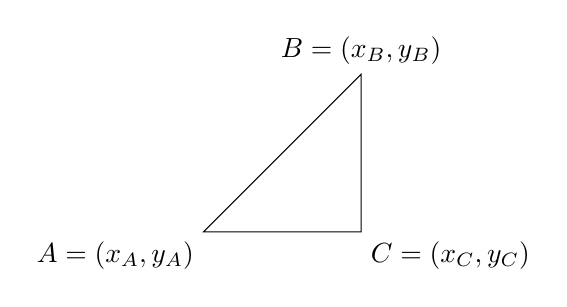
\begin{tikzpicture}[scale=0.5]
			\centering
		\draw (0,0) node[anchor=north east]{$A=(x_A,y_A)$}
			-- (4,0) node[anchor=north west]{$C=(x_C,y_C)$}
			-- (4,4) node[anchor=south]{$B=(x_B,y_B)$}
			-- cycle;
		\end{tikzpicture}
		... ci vorrebbe anche una spiegazione ... 
\end{enumerate}

\example
$$X=\R,\quad d(x_1,x_2)=\abs{x_2-x_1}$$
Le  proprietà 1,2,3 sono soddisfatte per le proprietà del modulo.\\
La proprietà 4 si può dimostrare: $$d(x_1,x_3)=\abs{x_3-x_1}\le\abs{x_3-x_2}+\abs{x_2-x_1}=d(x_3,x_2)+d(x_2,x_1)$$

\example
$$X=\bbsetn{R}{3}\quad d({x_1,y_1,z_1),(x_2,y_2,z_2)}$$
Analogo al primo esempio

\example
$$X=\bbsetn{R}{n}\quad$$
$$x=(x_1,\ldots,x_n) \quad\quad y=(y_1,\ldots,y_n)$$
$$d(x,y)=\sqrt{\sum\limits_{i=1}^{n}{\left(y_i-x_i\right)}^2}$$
Analogo al primo esempio

\example
$$X=\cntclass{0}(\realintervalclose{a}{b},\R),a,b\in\R, a<b$$
$$d_\infty=\sup\limits_{x\in\realintervalclose{a}{b}}\abs{g(x)-f(x)}$$
\begin{enumerate}
	\item $X$ contiene infiniti elementi(funzioni)
	\item $d_\infty$ è detta distanza uniforme o distanza della convergenza infinita o distanza della convergenza uniforme
	\item 
		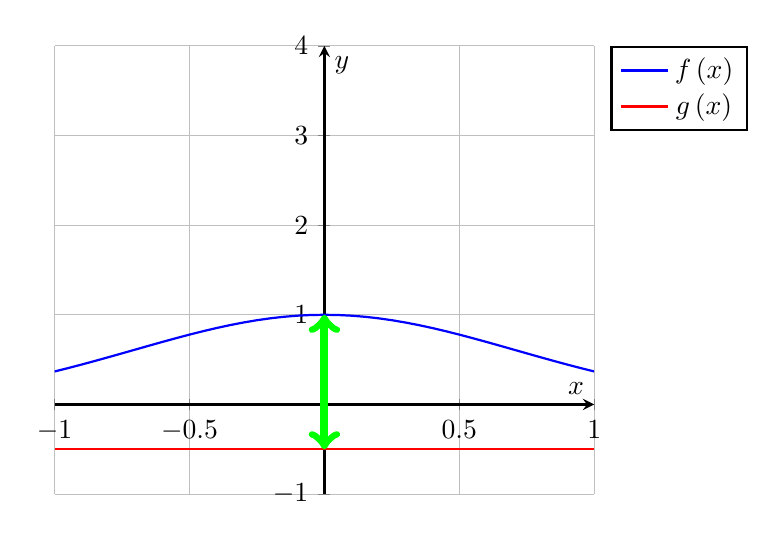
\begin{tikzpicture}[scale=1]
			\begin{axis}[
				xlabel={$x$},ylabel={$y$},
				axis lines=middle,
				samples=41,grid,thick,
				domain=-1:1,
				ymin=-1,ymax=4,
				legend pos=outer north east ]
				\addplot+[no marks] {e^-(abs(x*x))}; \addlegendentry{$f\left( x \right)$}
				\addplot+[no marks] {-0.5}; \addlegendentry{$g\left( x \right)$}
				\draw[<->,line width=1mm, color=green] (axis cs:0,-0.5) -- (axis cs:0,1);
			\end{axis}
		\end{tikzpicture}
\end{enumerate}
Si verificano le 4 proprietà di distanza:
\begin{enumerate}
	\item Se $\sup = \infty$ non va bene poiché l'insieme di arrivo è $\R$, applicando il Thm. di Weierstrass, una funzione continua definita su un intervallo $\realintervalclose{a}{b}$ ammette massimo e minimo e quindi anche il $\sup$ ....(le funzioni sono definite su un intervallo chiuso e limitato e sono continue)
	\item se e solo se hanno lo stesso dominio e per ogni punto di esso entrambe le funzioni hanno la stessa immagine
	\item $\dinfty{f}{g}=\ddinfty{f}{g}{\realintervalclose{a}{b}}=\ddinfty{g}{f}{\realintervalclose{a}{b}}=\dinfty{g}{f}$
	\item $\abs{h(x)-f(x)}\le\abs{h(x)-g(x)}+\abs{g(x)-f(x)} $, applicando il sup la disuguaglianza resta vera
\end{enumerate}
\observation 
Tutto questo è valido finché $\realintervalclose{a}{b}$ chiuso e limitato altrimenti non vale più Weierstrass \\
\\
UN CONTROESEMPIO\\
\\
\example
ferrovia
\example
Metrica Discreta
$X\ne \emptyset,\quad d(x,y)= \left\{\begin{matrix}0&&x=y\\0&&1\ne y\end{matrix}\right.$
	\begin{enumerate}
		\item $d(x,y)\ge 0$ per definizione
		\item $d(x,y)=0\sse x=y$, per definizione (ragiona sul sse) 
		\item $d(x,y)=d(y,x)$ ...per definizione (fai due casi x=y e l'altro)
		\item $d(x,y)\le d(y-z)+d(z-x)$ 
	\end{enumerate}
\example
$$X=\bbsetn{R}{2}$$
$$x=(x_1,x_2), y=(y_1,y_2)$$
$$d'(x,y)=\abs{x_1-y-1}+\abs{x_2-y-2}$$
...\\

\example
\example
$$X=\cntclass{0}(\realintervalclose{0}{1},\R)$$
$$d_2=\int_0^1\abs{g(x)-f(x)}d(x)$$
\example
$$X=\cntclass{0}(\realintervalclose{a}{b},\R), a,b\in\R, a<b$$
$$d_2=\sqrt{\int_a^b\left[g(x)-f(x)\right]^2d(x)}$$

\proposition
Sia $(X,d)$ s.m. e $A\subseteq X$ e $A\ne \emptyset$, sia $\begin{array}{rcl} d_{|A} : A\times A & \to & \mathbb{R} \\ (x,y) & \to & d(x,y) \end{array} \Rightarrow (A,d_{|A})$ è uno spazio metrico
\begin{proof}
	........
\end{proof}

\definition
Un insieme è finito se il numero dei suoi elementi è finito
\definition
Un insieme è infinito se non è finito
\definition
Sia $(X,d)$s.m., $A\subseteq X$, $A\ne \emptyset$ si definisce diametro di A: $$diam(A)=\sup\limits_{x,y\in A}d(x,y)$$
\definition
$A$ è limitato $\leftrightharpoons diam(A)$ è finito ($\in\R$)
\definition
$A$ è illimitato $\leftrightharpoons diam(A)$ è infinito ($=\infty$)
\example
...\\
...\\
...\\
..\\
....\\
\observation
Ogni insieme finito è limitato e ogni insieme illimitato è infinito. Non valgono i viceversa.
\example 
.....\\
....\\
.....\\
......\\
.....\\
....\\

\definition
$X$ è uno spazio (vettoriale) normato sul campo $\bbset{K}$ se:
\begin{description}
	\item[$\bullet$] $X$ è uno spazio vettoriale sul campo $\bbset{K}$
	\item[$\bullet$] se è definita una norma su $X$, ovvero una funzione\\
	$\norm{\cdot}:X\to\R$ con le seguenti proprietà:
	\begin{enumerate}
		\item $\forall x\in X,\quad\norm{x}\ge0$
		\item $\forall x\in X,\quad\norm{x}=0\sse x=0$
		\item $\forall x,y\in X,\quad\norm{x+y}\le\norm{x}+\norm{y}$
		\item $\forall x\in X,\lambda\in\bbset{K},\quad\norm{\lambda x}=\abs{\lambda}\cdot\norm{x}$
	\end{enumerate}
\end{description}

\begin{example}
$$X=\R\quad\norm{x}=\abs{x}$$
\end{example}
\begin{example}
	$$X=\bbsetn{R}{2}\quad\norm{\left[\begin{matrix}x\\y+\end{matrix}\right]}=\sqrt{x^2+y^2}$$
\end{example}
\begin{example}
	$$X=\bbsetn{R}{n}\quad x\equiv(x_1,\ldots,x_n)\quad \norm{x}=\sqrt{\sum\limits_{i=0}^n}x_i^2$$
\end{example}
\begin{example}
	$$X=\bbset{C}\quad\norm{x}=\abs{x}$$
\end{example}
\begin{example}
	$$X=\cntclass{0}(\realintervalclose{a}{b},\R)\quad\norm{f}\sup\limits_{x\in\realintervalclose{a}{b}}\abs{f}$$
\end{example}

\proposition
Sia $X$ uni spazio normato allora $(X,d)$ è uno spazio metrico con $\begin{array}{rcl} d : X\times X & \to & \mathbb{R} \\ (x_1,x_2) & \to & \norm(x_1-x_2) \end{array}$\\
Inoltre per la distanza così definita valgono le seguenti proprietà:
\begin{enumerate}
	\item INVARIANZA PER TRASLAZIONI
	$$\forall x_1,x_2,x_3\in X \quad d(x_1,x_2)=d(x_1+x_3,x_2+x_3)$$
	\item POSITIVAMENTE OMOGENEA
	$$ \forall x_1,x_2\in X, \lambda\in\R\quad d(\lambda x_1,\lambda x_2)=\abs{\lambda}d(x_1,x_2)$$
\end{enumerate}
\begin{proof}
	Per dimostrare che è uno spazio metrico si dimostra che valgono le proprietà di distanza
	\begin{enumerate}
		\item
		\item
		\item
		\item
	\end{enumerate}
\end{proof}

\definition
Sia $(X,d)$ spazio metrico e siano $x_0\in X$ e $r\in\bbset{r}$. Si dice sfera aperta di centro $x_0$ e raggio $r$ l'insieme:
$$B(x_0,r)=\left\{ x\in X : d(x,y)<r  \right\}$$
\observation
se $r=0\Rightarrow B(x_0,r)=\emptyset$\\
se $r>0\Rightarrow x_0\in B(x_0,r)$
\example
In $\R$ con $d_E$, $B(x_0,r)$ è un intervallo simmetrico centrato in $x_0$
\example
In $\bbsetn{R}{2}$ con $d_E$, $B(x_0,r)$ è una un cerchio con centro in $x_0$
\example
In $\bbsetn{R}{3}$ con $d_E$, $B(x_0,r)$ è una sfera con centro in $x_0$
\example

% TODO le definizioni prima di questa nel capitolo 1
\begin{definition}
	\label{def:aperto}
	Sia $(X,d)$ spazio metrico, sia $A\subseteq X$. Si definisce
	$$A\text{ è \textbf{aperto}}\bydef A=\emptyset\quad\text{oppure}\quad A=\circdot{A}$$
\end{definition}

\begin{definition}
	\label{def:chiuso}
	Sia $(X,d)$ spazio metrico, sia $A\subseteq X$. Si definisce
	$$A\text{ è \textbf{chiuso}}\bydef A=\emptyset\quad\text{oppure}\quad A=\bar{A}$$
\end{definition}

\definition
Siano $(X,d_1)$ e $(X,d_2)$ spazi metrici. $d_1$ e $d_2$ sono equivalenti $\leftrightharpoons \exists c,C\in\R, c_1>0, c_2>0$ t.c:
$$ \forall x,y \in X\quad cd_1(x,y)\le d_2(x,y)\le Cd_1(x,y) $$


\section{Successioni e Completezza}
\begin{definition}
	% TODO Definizione successione
\end{definition}
\begin{definition}
	% TODO Successione limitata
\end{definition}
\begin{definition}
	% TODO Successione convergente
\end{definition}
\begin{proposition}
	\label{prop:succ_conv_lim}
	Data la successione $x: \N \mapsto X$ di elementi dello spazio metrico $(X,d)$ e dato $x_\infty\in X$:
	$$\lim\limits_{n\rightarrow+\infty}x_n=x_\infty\iff\forall\varepsilon > 0\;\;\exists\nu\in\N:\quad\forall n>\nu\;\;d(x_n,x_\infty)<\varepsilon$$
	\begin{proof}
		% TODO dimostrazione
	\end{proof}
\end{proposition}
\subsection{Insiemi Compatti}
\begin{definition}[Insieme Compatto]
	\label{def:compatto}
	Sia $(X,d)$ uno spazio metrico e sia $A \subseteq X$. $A$ è compatto se e solo se ogni successione di elementi di $A$ ammette una sottosuccessione avente limite in $A$.
	\begin{note}
		Questa è la definizione di \textbf{Compattezza per Successioni}, in spazi più generali può essere necessario utilizzare una definizione più debole che, nel caso degli spazi metrici, coincide con la precedente.
	\end{note}
\end{definition}

\section{Limiti e Continuità}
\begin{definition}
	Siano $(X,d_x)$ e $(Y,d_y)$ spazi metrici, $A\subseteq{X}$,$x_0$ di accumulazione per $A$, $f:A\rightarrow{Y}$ una funzione e $l\in{Y}$ \\
	$\lim\limits_{x \rightarrow x_0} = l \rightleftharpoons \forall{\varepsilon},\exists\delta : \forall{x}\in A : d_x(x,x_0)<\delta e x\ne{x_0} : d_y(f(x),l)<\varepsilon$
\end{definition}

\begin{proposition}
	Siano $(X,d_x)$ e $(Y,d_y)$ spazi metrici, $A\subseteq{X}$,$x_0$ di accumulazione per $A$, $f:A\rightarrow{Y}$ una funzione e $l'\in{Y}$,$l''\in{Y}$
\end{proposition}

\begin{definition}[Funzione Continua]
	\label{def:funz_cont}
	Siano $(X,d_X)$ e $(Y,d_Y)$ spazi metrici e sia $f: A \mapsto Y$ con $A \subseteq X$ e sia $x_0 \in A$
	\begin{equation*}
		\begin{gathered}
			f \text{ è \textbf{continua} in } x_0 \iff\\
			\forall \varepsilon > 0\;\;\exists \delta > 0:\quad \forall x \in A \text{ con } d_X(x,x_0)<\delta \text{ vale } d_Y \bigl(f(x),f(x_0)\bigr) < \varepsilon
		\end{gathered}
	\end{equation*}

	\begin{center}
		$f$ è \textbf{continua} in $A\bydef$\\
		$f$ è continua \textbf{in ogni punto} di $A$
	\end{center}
	\begin{note}
		Non andrebbe detto semplicemente $f$ \textit{è continua} perché la continuità dipende in modo essenziale dall'insieme di punti su cui la funzione viene considerata. In assenza di ulteriori specificazioni, spesso si sottointende che l'insieme in esame è l'intero dominio della funzione.
	\end{note}
	\begin{note}
		Ha senso valutare la continuità di una funzione esclusivamente nell'insieme in cui è definita. Quindi una frase come:\\
		\textit{la funzione} $x \mapsto \frac{1}{x}$ \textit{è discontinua in} $0$,\\
		non è (a rigore) sensata. Andrebbe riformulata come:\\
		\textit{la funzione} $x \mapsto \frac{1}{x}$ \textit{non può essere estesa ad una funzione definita e continua anche in} $0$.
	\end{note}
	\begin{note}
		La continuità di una funzione dipende in modo esssenziale anche dalla distanza adottata, tuttavia è prassi sottointendere questa precisazione, soprattutto per funzioni $\R^n \mapsto \R^n$, se la distanza adottata è quella Euclidea.
	\end{note}
\end{definition}

\begin{theorem}[Teorema generale di Weierstrass]
	\label{teo:weier_generale}
	Siano $(X,d_X)$ e $(Y,d_Y)$ spazi metrici e sia $f:K \mapsto Y$ con $K \subseteq X$.
	$$\left.\begin{array}{ll}
		K \text{compatto} \\
		f \text{continua su } K
		\end{array} \quad\right\} \implies f(K) \text{compatto}$$
	\begin{proof}
		Siano le successioni
		\begin{itemize}
			\item $y: \N \mapsto Y$ tale che $y_n \in f(K) \;\forall n \in \N$, cioè $\forall n \in \N\;\exists x_n \in K: f(x_n) = y_n$
			\item $x: \N \mapsto X$ tale che $x_n \in K\;\forall n \in \N$
		\end{itemize}
		\begin{note}
			Abbiamo una successione che, attraverso la $f$ (non direttamente: le successioni non sono $X \mapsto Y$!), associa indirettamente valori in $K \subseteq X$ a valori in $f(K) \subseteq Y$
		\end{note}
		La successione $x$ ammette una sottosuccessione $x_{n_k}$ convergente ad un elemento $\overline{x} \in K$ dalla \fullref{def:compatto}, avendo $K$ compatto per ipotesi, ed essendo $x$ a valori in $K$.\\
		Data la continuità di $f$ in $K$, abbiamo $y_{n_k} = f(x_{n_k}) \in f(K)$, ma essendo $x_{n_k}$ convergente ad $\overline{x}$, anche $y_{n_k}$ converge, verificando così la definizione di spazio Compatto.
	\end{proof}
	\begin{proof} (Alternativa)\\
		La successione $x$ ammette una sottosuccessione $x_{n_k}$ convergente ad un elemento $\overline{x} \in K$, dunque da \Cref{prop:succ_conv_lim}:
		$$\lim\limits_{n\rightarrow+\infty}x_n=x_*\iff\forall\eta > 0\;\;\exists\nu\in\N:\quad\forall n>\nu\;\;d(x_n,x_*)<\eta$$
		Dalla \fullref{def:funz_cont} e sapendo che $f(x)$ è continua, sappiamo che:
		$$\forall\varepsilon > 0\;\;\exists\delta > 0:\quad\forall x \in K\;\;d_X (x,x_*)<\delta\;\;d_Y \bigl(f(x_n),f(x_*)\bigr)<\varepsilon$$
		Unisco ora le due definizioni:
		$$\forall \varepsilon > 0\;\;\exists \nu \in \N:\quad \forall n > \nu\;\;d_Y \bigl(f(x_n),f(x_*)\bigr)<\varepsilon$$
		Che equivale, per come è definita $y_n$, a
		$$\lim\limits_{n\rightarrow +\infty}y_n = y_*$$
		Cioè la definizione di successione convergente. Ho dunque individuato una sottosuccessione convergente per ogni successione in $f(K)$, verificando così la definizione di spazio Compatto.
	\end{proof}
\end{theorem}

\section{Il Teorema delle Contrazioni}
\begin{definition}[Contrazione]
	\label{def:contrazione}
	Sia $(X, d)$ uno spazio metrico. Si dice contrazione una funzione T: $X \mapsto X$ soddisfacente a:
	\begin{align}
		\label{equaz:def_contrazione}
		\exists K \in [0, 1[\;\text{tale che}\;\forall x',x''\in X\;\text{vale}\\
		d_X(T(x''), T(x')) \le K \cdot d_X(x'', x').
	\end{align}


	Una contrazione è quindi una funzione con insieme di partenza e di arrivo coincidenti e
	Lipschitziana con costante di Lipschitz strettamente minore di 1.
	E generalmente inutile considerare contrazioni definite tra spazi diversi. Data una funzione
	$T: X\rightarrow Y$ Lipschitziana, è sempre possibile riscalare la distanza in uno dei due spazi X o Y
	per ottenere una costante di Lipschitz minore di 1.
	\begin{note}
		D'ora in poi si utilizzerà la notazione $Tx$ per intendere $T(x)$
	\end{note}
\end{definition}

ESEMPI:\\
\begin{enumerate}
	\item $f: \R \rightarrow \R$ data da $f(x) = \frac{x}{2}$. $f$ è una contrazione.
	\item $f: [0,2] \rightarrow [0,2]$ data da $f(x) = 1+\frac{x}{2}. f$ è una contrazione
	\item $f: \R^2 \rightarrow \R^2$ data da $f(x,y)=\begin{bmatrix} \frac{1}{3}&&0\\0&&\frac{1}{5}\end{bmatrix}$ è una contrazione
\end{enumerate}

\proposition
Sia $(X, d)$ uno spazio metrico, siano $f,g:X\rightarrow X$ due contrazioni in $X \Rightarrow f\circ g$ è una contrazione
\begin{proof}
	Sappiamo che\\
	$$\forall x',x''\in X, d(fx'', fx')\le K_fd(x'', x').$$
	$$\forall x',x''\in X, d(gx'', gx')\le K_gd(x'', x').$$
	$f\circ g=f(g(x))$, quindi presi $x',x''\in X$ si ha che: $$d(fg(x''), fg(x'))\le K_fd(g(x''), g(x'))\le K_fK_gd(x'',x').$$
\end{proof}

\proposition
Sia $f \in C1(R^n;R^n)$. Se $\exists k \in [0, 1[$ tale che $\forall x \in \R^n$ vale $\norm{Df(x)}  < k$, allora $f$ è una contrazione.

\begin{theorem}[Teorema delle Contrazioni]
	\label{teo:contrazioni}
	Sia $(X, d)$ uno spazio metrico completo in cui è definita una contrazione
	$T: X \rightarrow X$. Allora esiste un unico punto fisso di $T$ in $X$.
	\begin{proof}
		Costruisco una successione di elementi di $X$ nel seguente modo:\\
		scelgo $x_0\in X$,\\
		$x_1 = Tx_0$\\
		$x_2 = Tx_1$\\\\
		...\\
		$x_n = Tx_{n-1}$\\
		La successione ${x_n: n \in N }$ così costruita è una successione di Cauchy. Infatti, presi $n, m \in N$ con $m > n$ si ha:
		$$d(x_{m},x_{n}) = d(Tx_{m-1},x_{n-1}) \le Kd(x_{m-1},x_{n-1})=$$
		$$=Kd(x_{m-1},x_{n-1}) = Kd(Tx_{m-2},x_{n-2}) \le K^2d(x_{m-2},x_{n-2})=$$
		$$=...=$$
		$$=...=K^nd(x_{m-n},x_{0})\le$$
		$$\le K^{n}\sum\limits_0^{m-n+1}(d(x_{m-n-i},x_{m-n-i-1}))=$$
		$$\le \sum\limits_0^{m-n+1}(d(Tx_{m-n-i-1},Tx_{m-n-i-2}))$$
		per ogni termine di questa sommatoria si può applicare lo stesso ragionamento
		$$\le K^{n}\sum\limits_0^{m-n+1}(K^{m-n-2}d(Tx_{0},x_{0}))=$$
		$$\le K^{n}d(Tx_{0},x_{0})\sum\limits_0^{m-n+1}K^{m-n-2}=K^n\frac{1-K^{m-n-1}}{1-K}d(Tx_{0},x_{0}) \le \frac{K^n}{1-K}d(Tx_{0},x_{0})$$
		Ho quindi trovato che $d(x_{m},x_{n})\le\frac{K^n}{1-K}d(Tx_{0},x_{0})$\\
		L’ultima espressione ottenuta può essere resa arbitrariamente piccola (in modulo) pur di
		prendere $n$, e quindi anche $m$, sufficientemente elevato. La completezza di $X$ implica quindi
		che esiste il limite $\lim\limits_{n\rightarrow +\infty}xn$. Sia $x^*$ questo limite. $x^*$ è un punto fisso per $T$. Infatti, grazie
		alla continuità di $T$:
		$$T(x^*)=T{\lim\limits_{n\rightarrow +\infty}xn}$$
	\end{proof}
\end{theorem}

\begin{definition}[Funzione Iterata]
	\label{def:iterata}
	Data $F:X\mapsto X$, si dice funzione iterata $n$ volte di $F$ la $F^n$ che corrisponde all'applicazione $n$ volte di $F$ su sè stessa. Formalmente:
	$$f^{n+1} = f \circ f^n \quad \forall n \in \N\setminus\brackets{0}$$
	Se $n = 0$, per definizione, $f^0 = \mathrm{Id}_X$ con $\mathrm{Id}_X$ funzione identità su $X$
\end{definition}

\begin{theorem}[Teorema dell'Iterata Contrazione]
	\label{teo:teo_iterata_contraz}
	Sia $(X,d_X)$ uno spazio metrico completo e sia $T:X\mapsto X : \exists n \in \N, T^n$ \textbf{iterata} è contrazione.\\
	Allora $T$ ammette un unico punto fisso in $X$
	\begin{note}
		La $n$ non è univocamente definita e non potrebbe esserlo. Se infatti $T^n$ è contrazione, allora anche $T^{2n},\, T^{3n},\, \cdots,\, T^{\alpha n}$ lo sono.
	\end{note}
	\begin{proof}
		Per il \fullref{teo:contrazioni} esiste un unico punto fisso $x_* \in X$ per $T^n$, quindi
		$$T^nx_* = x_*$$
		applicando $T$ ad entrambi i membri
		$$T(T^{n}x_*) = Tx_*$$
		e per la \fullref{def:iterata}
		$$T(T^{n}x_*) = T^n(Tx_*) = Tx_*$$
		Dunque $Tx_*$ è punto fisso della $T^n$. Avevamo però già trovato che $x_*$ era punto fisso della $T^n$ e, per il \fullref{teo:contrazioni}, può esistere un unico punto fisso. Ciò permette di concludere che $Tx_* = x_*$
	\end{proof}
\end{theorem}

\section{Funzioni a Valori in $\protect\mathbb{R}$}
%TODO This section is a placeholder
\part{Calcolo Differenziale}

\chapter{Calcolo Differenziale}

\section{Preliminari}
La base canonica di $R^n$ è indicata con $(e_1,...,e_i)$, $e_i$ è il vettore di $R^n$ con tutte le componenti nulle tranne la i-esima che vale 1.\\
Un generico vettore $x$ si può quindi scrivere come combinazione lineare dei vettori di base $x=\sum\limits_{j=1}^{i}\alpha_j e_j$.\\
Nel caso n=2 è usata la notazione $(x,y)=xi+yj$\\
Nel caso n=3 è usata la notazione $(x,y,z)=xi+yj+zk$\\
Alcune classi di funzioni $f:A\subseteq\R^n\rightarrow\R^m$ hanno nomi particolari:
\begin{itemize}
	\item 
	$n=1$,$m=1$:$f$ è una funzione reale di una variabile reale;
	\item 
	$n=1$,$m>1$:$f$ è una curva in $R^m$ (purché sia almeno continua e definita su un intervallo)
	\item 
	$n>1$,$m=1$:$f$ è un campo scalare
	\item
	$n>1$,$m>1$:$f$ è un campo vettoriale
\end{itemize}
\section{Derivate Parziali e Direzionali}
\definition
sia $f:A\subseteq\R^2\rightarrow\R$ e $(x_0,y_0)\in\circdot{A}$, $h,k\in\R$
chiamo derivata parziale rispetto a $x$ di $f$ in $(x_0,y_0)$ la quantità (se esiste finita)
$$\partial_xf(x_0,y_0) = \lim\limits_{h\rightarrow{0}}\frac{f(x_0+h,y_0)-f(x_0,y_0)}{h}$$
chiamo derivata parziale rispetto a $y$ di $f$ in $(x_0,y_0)$ la quantità (se esiste finita)
$$\partial_yf(x_0,y_0) = \lim\limits_{h\rightarrow{0}}\frac{f(x_0,y_0+k)-f(x_0,y_0)}{h}$$
\definition
sia $f:A\subseteq\R^n\rightarrow\R^m$ e $x_0\in\circdot{A}$, $i=1,...,n$
$$\partial_if(x_0) = \lim\limits_{t\rightarrow{0}}\frac{f(x_0+te_i)-f(x_0)}{t}$$
dove $(e_1,...,e_n)$ rappresentano la base canonica di $R^n$\\
\observation nella prima definizione la derivata è un valore reale mentre nella seconda è un vettore di $R^m$\\
\observation le proprietà e le regole di derivazione sono le stesse di Analisi 1
\definition
sia $f:A\subseteq\R^2\rightarrow\R$ e $(x_0,y_0)\in\circdot{A}$, sia $v\in\R^2 con \norm{v}=1 $
diciamo derivata nella direzione $v$ della funzione $f$ nel punto $(x_0,y_0)$ il limite (se esiste finito)\\
$$D_vf(x_0,y_0) = \lim\limits_{t\rightarrow{0}}\frac{f(x_0+tv_1,y_0+tv_2)-f(x_0,y_0)}{t}$$
dove $v_1,v_2$ sono le componenti di $v(v=\begin{bmatrix}v_1\\v_2\end{bmatrix})$
\definition
sia $f:A\subseteq\R^n\rightarrow\R^m$ e $x_0\in\circdot{A}$, sia $v\in\R^n con \norm{v}=1 $
diciamo derivata nella direzione $v$ della funzione $f$ nel punto $x_0$ il limite (se esiste finito)\\
$$D_vf(x_0) = \lim\limits_{t\rightarrow{0}}\frac{f(x_0+tv)-f(x_0)}{t}$$
\proposition
(ANALISI 1): sia $f:A\subseteq \R\rightarrow\R$ e $x_0\in\circdot{A}$\\
$f$ è differenziabile $\Leftrightarrow$ $\exists m\in \R $ t.c. $f(x_0+h)=f(x_0)+mh+o(h)$ per $h\rightarrow 0$
...\\
...\\
...\\
\begin{exercise}
	\label{ex:funz_derivabili}
	Formulare in modo rigoroso e dimostrare:
	\begin{enumerate}
		\item La somma di funzioni parzialmente derivabili è parzialmente derivabile.
		\item La composizione di funzioni parzialmente derivabili è parzialmente derivabile.
		\item Prodotto e rapporto, quando definiti, di funzioni parzialmente derivabili sono funzioni parzialmente derivabili.
	\end{enumerate}
	% TODO soluzione
\end{exercise}

\section{Derivata Totale}
\definition
sia $f:A\subseteq \R^n\rightarrow \R^m$ e $x_0\in\circdot{A}$ \\
$f$ è differenziabile in $x_0\rightleftharpoons$ $\exists M\in Mat(mxn) : f(x_0+h) = f(x_0)+Mh+o(h)$ per $h\rightarrow 0$ 
\definition
siano $f,g : A\subseteq \R^n\rightarrow \R^m$ e $x_0$ di accumulazione per A \\
$f=o(g)$ per $x\rightarrow x_0 \rightleftharpoons \lim\limits_{x->x_0}\frac{\norm{f(x)} }{\norm{g(x)} }$
\definition
sia $f:A\subseteq \R^2\rightarrow \R$ e $(x_0,y_0)\in\circdot{A}$ \\
$f$ è differenziabile in $(x_0,y_0)\rightleftharpoons$ $f(x_0+h,y_0+k) = f(x_0)+m_1h+m_2k+o(\sqrt{h^2+k^2})$ per $(h,k)\rightarrow (0,0)$
\definition
siano $f,g : :A\subseteq \R^2\rightarrow \R$ e $(x_0,y_0)$ di accumulazione per $A$ \\
$f=o(g)$ per $(x,y)\rightarrow (x_0,y_0) \rightleftharpoons \lim\limits_{(x,y)->(x_0,y_0)}\frac{\norm{f(x,y)} }{\norm{g(x,y)} }$
\proposition{(Unicità della derivata totale)}
sia $f:A\subseteq \R^n\rightarrow \R^m$, $x_0\in\circdot{A}$, $M_1$,$M_2\in Mat(mxn)$\\
$M1$ derivata totale di $f$ in $x_0$,\\
$M2$ derivata totale di $f$ in $x_0$,\\
allora $M1=M2$\\
\begin{proof}
	poiché $M_1$ e $M_2$ sono derivate totali di $f$ nel punto $x_0$,\\
	$f(x_0+h) = f(x_0)+M_1h+o(h)$ per $h\rightarrow 0$\\
	$f(x_0+h) = f(x_0)+M_2h+o(h)$ per $h\rightarrow 0$\\
	facendo la differenza membro a membro delle precedenti ottengo che $(M_1-M_2)h=o(h)$ per $h\rightarrow 0$\\
	Scelto $h=te_i$, dove $e_i$ è un vettore della base canonica, si ottiene $(M_1-M_2)te_i=o(h)$ quindi\\
	$\lim\limits_{t\rightarrow 0}\frac{(M_1-M_2)te_i}{t\norm{e_i} } = \lim\limits_{t\rightarrow 0}(M_1-M_2)e_i = 0$, poiché $e_i$ è un vettore non nullo deve essere $(M_1-M_2)=0$ quindi $M_1 = M_2$\\
\end{proof}
\observation
L'ultima riga della dimostrazione dice che le applicazioni lineari $M_1$ e $M_2$ hanno le stesse immagini sui vettori della base canonica, quindi coincidono.

\proposition
sia $f:A\subseteq \R^n\rightarrow \R^m$, $x_0\in\circdot{A}$\\
$f$ è differenziabile in $x_0$ $\Rightarrow$ $f$ è continua in $x_0$\\
DIMOSTRAZIONE\\

..\\
..\\
..\\
..\\
..\\
..\\


\theorem{Differenziale Totale}
sia $f:A\subseteq \R^n\rightarrow \R^m$ e $x_0\in\circdot{A}$.\\
$\exists \partial_{i}f(x)\;\forall i=1,...,n definite \forall x$ in un intorno di $x_0$\\
$\partial{i}f$ è continua in $x_0$\\
$\Rightarrow f$ è differenziabile in $x_0$\\

\theorem{Differenziale Totale}
sia $f:A\subseteq \R^2\rightarrow \R$ e $(x_0,y_0)\in\circdot{A}$.\\
$\exists \partial_{x}f(x,y)$ e $\exists \partial_{y}f(x,y)$ definite $\forall x$ in un intorno di $(x_0,y_0)$\\
$\partial_{x}f(x,y)$ e $\exists \partial_{y}f(x,y)$ continue in $x_0$\\
$\Rightarrow f$ è differenziabile in $(x_0,y_0)$\\
\begin{proof}
	devo dimostrare che
	$$\lim\limits_{(h,k)\rightarrow (0,0)}\frac{f(x_0+h,y_0+k)-f(x_0,y_0)-\nabla f(x_0,y_0\begin{bmatrix}h\\k\end{bmatrix})}{\sqrt{h^2+k^2}} = 0$$
	dove $\nabla f(x_0,y_0)= \begin{bmatrix}\partial_xf(x_0,y,0) && \partial_yf(x_0,y_0)\end{bmatrix}$\\

	\begin{tikzpicture}
	\pgfmathsetmacro\MAX{8}
	\pgfmathsetmacro\XZ{\MAX / 3 }
	\pgfmathsetmacro\YZ{\MAX / 3 }
	\pgfmathsetmacro\XZh{\MAX / 3 *2}
	\pgfmathsetmacro\YZk{\MAX / 3 *2}
	\coordinate (X0Y0) at (\XZ,\YZ);
	\coordinate (X0hY0) at (\XZh,\YZ);
	\coordinate (X0Y0k) at (\XZ,\YZk);
	\coordinate (X0hY0k) at (\XZh,\YZk);
	
	\draw[->] (0,0) -- (\MAX,0) node[anchor=north west] {x};
	\draw[->] (0,0) -- (0,\MAX) node[anchor=south east] {y};
	\draw[dotted] (\XZ,0) -- (\XZ,\MAX);
	\draw[dotted] (0,\YZ) -- (\MAX,\YZ);
	\draw[dotted] (\XZh,0) -- (\XZh,\MAX);
	\draw[dotted] (0,\YZk) -- (\MAX,\YZk);
	\draw node[anchor=north] at (\XZ,0) {$x_0$};
	\draw node[anchor=north] at (\XZh,0) {$x_0+h$};
	\draw node[anchor=east] at (0,\YZ) {$y_0$};
	\draw node[anchor=east] at (0,\YZk) {$y_0+k$};
	\draw node at (X0Y0) {$\bullet$};
	\draw node at (X0Y0k) {$\bullet$};
	\draw node at (X0hY0) {$\bullet$};
	\draw node at (X0hY0k) {$\bullet$};
	\draw node[anchor=north east] at (X0Y0) {$(x_0,y_0)$};
	\draw node[anchor=south east] at (X0Y0k) {$(x_0,y_0+k)$};
	\draw node[anchor=north west] at (X0hY0) {$(x_0+h,y_0)$};
	\draw node[anchor=south west] at (X0hY0k) {$(x_0+h,y_0+k)$};
	
	\draw[<-] (\XZ,\MAX*4/10) -- (\XZ,\MAX*6/10);
	\draw[<-] (\XZh,\MAX*4/10) -- (\XZh,\MAX*6/10);
	\draw[<-] (\MAX*4/10,\YZ) -- (\MAX*6/10,\YZ);
	\draw[<-] (\MAX*4/10,\YZk) -- (\MAX*6/10,\YZk);
	
	\draw node at (\XZ,\MAX/2) {A};
	\draw node at (\XZh,\MAX/2) {B};
	\draw node at (\MAX/2,\YZ) {C};
	\draw node at (\MAX/2,\YZk) {D};
	\end{tikzpicture}
	devo calcolare lo scarto della funzione tra i punti $(x_0+h,y_0+k)$ e $(x_0,y_0)$. Ho a disposizione le derivate parziali che mi danno informazioni lungo le parallele agli assi quindi non muovo lungo la diagonale ma lungo i percorsi D,A e B,C\\
	Il limite  (<-) fa zero se il numeratore è zero, allora guardo solo quello.\\
	$$f(x_0+h,y_0+k) -f(x_0,y_0)- \partial{x}f(x_0,y_0)h - \partial{y}f(x_0,y_0)k$$
	riscrivo tale quantità seguendo il percorso D,A
	$$ [f(x_0+h,y_0+k) - f(x_0+h,y_0)] + [f(x_0+h,y_0) - f(x_0,y_0)] - \partial{x}f(x_0,y_0)h - \partial{y}f(x_0,y_0)k$$
	chiamo $\varphi (x) = f(x,y_0)$ quindi $f(x_0+h,y_0)-f(x_0,y_0) = \varphi (x_0+h)-\varphi (x_0)$\\
	la funzione $\varphi $ è una funzione reale di una variabile reale ed in virtù del teorema di Lagrange $\varphi (x_0+h)-\varphi (x_0) = \varphi'(x_0 + \beta h)h$ per $\beta\in ]0,1[ $, per come definita $\varphi$ si ha che $\varphi'(x_0 + \beta h)h = \partial_{x}f(x_0+\beta h,y_0)h$\\
	con un ragionamento del tutto analogo si può definire $\varPsi (x) = f(x_0+h,y)$ e si ha che $\varPsi (y_0+h)-\varPsi (y_0) = \varPsi'(y_0 + \alpha k)k = \partial_{y}f(x_0+h,y_0+\alpha k)k$ per $\alpha\in ]0,1[ $\\
	Quindi
	$$ [f(x_0+h,y_0+k) - f(x_0+h,y_0)] + [f(x_0+h,y_0) - f(x_0,y_0)] - \partial{x}f(x_0,y_0)h - \partial{y}f(x_0,y_0)k = $$
	$$= [\partial_{x}f(x_0+\beta h,y_0)h] + [\partial_{y}f(x_0+h,y_0+\alpha k)k] - \partial{x}f(x_0,y_0)h - \partial{y}f(x_0,y_0)k = $$
	$$= [\partial_{x}f(x_0+\beta h,y_0)h - \partial{x}f(x_0,y_0)h] + [\partial_{y}f(x_0+h,y_0+\alpha k)k  - \partial{y}f(x_0,y_0)k] $$
	Adesso la riscrivo recuperando il denominatore 	'e devo verificare che il limite per $(h,k)\rightarrow (0,0)$ tenda a zero.\\
	
	$$[\partial_{x}f(x_0+\beta h,y_0)-\partial{x}f(x_0,y_0)] \frac{h}{\sqrt{h^2+k^2}} + [\partial_{y}f(x_0+h,y_0+\alpha k) - \partial{y}f(x_0,y_0)]\frac{k}{\sqrt{h^2+k^2}} $$
	Le derivate parziali sono continue quindi per $(h,k)\rightarrow (0,0)$ i numeratori tendono a zero\\
	Inoltre le due frazioni per $(h,k)\rightarrow (0,0)$ sono quantità limitate tra $-1$ e $1$ quindi si può dire che il limite cercato fa 0.
\end{proof}


\subsection{Regole di Derivazione}
\proposition
Siano $f,g: A\subseteq \R^n \rightarrow \R^m$ e $x_0\in\circdot{A}$\\
$f$ differenziabile in $x_0$, $g$ differenziabile in $x_0$ allora $f+g$ differenziabile in $x_0$ e $D(f+g)(x_0) = Df(x_0)+Dg(x_0)$
\begin{proof}
	$f$ è differenziabile, allora $f(x_0+h)=f(x_0)+Df(x_0)h+o(h)$ per $h\rightarrow 0$\\
	anche $g$ lo è, quindi $g(x_0+h)=g(x_0)+Dg(x_0)h+o(h)$ per $h\rightarrow 0$\\
	sommando membro a membro si ottiene  $(f+g)(x_0+h)=(f+g)(x_0)+[Df(x_0)+Dg(x_0)]h+o(h)$ per $h\rightarrow 0$\\
	Questa è la definizione di differenziabilità, allora $f+g$ è differenziabile e $D(f+g)(x_0) = Df(x_0)+Dg(x_0)$
\end{proof}

\proposition
Sia $f: A\subseteq \R^n \rightarrow \R^m$ e $x_0\in\circdot{A}$ e $\lambda\in \R$\\
$f$ differenziabile in $x_0$ allora $\lambda f$ differenziabile in $x_0$ e $D(\lambda f)(x_0) = \lambda Df(x_0)$
\begin{proof}
	$f$ è differenziabile, allora $f(x_0+h)=f(x_0)+Df(x_0)h+o(h)$ per $h\rightarrow 0$\\
	valuto ora $(\lambda f)(x_0+h)=(\lambda f)(x_0)+\lambda Df(x_0)h+o(h)$ per $h\rightarrow 0$\\
	Questa è la definizione di differenziabilità, allora $\lambda f$ è differenziabile e $D(\lambda f)(x_0) = \lambda Df(x_0)$
\end{proof}

\proposition
Sia $g: A\subseteq \R^n \rightarrow \R^m$ e $x_0\in\circdot{A}$\\
Sia $f: B\subseteq \R^m \rightarrow \R^p$ e $g(x_0)\in\circdot{B}$\\
$f$ differenziabile in $g(x_0)$, $g$ differenziabile in $x_0$ allora $f\circ g$ differenziabile in $x_0$ e $D(f\circ g)(x_0) = Df(g(x_0))*Dg(x_0)$
\begin{proof}
	$g$ è differenziabile in $x_0$, allora $g(x_0+h)=f(x_0)+Dg(x_0)h+o(h)$ per $h\rightarrow 0$\\
	$f$ è differenziabile in $g(x_0)$ allora $g(g(x_0)+k)=f(g(x_0))+Df(g(x_0))k+o(k)$ per $k\rightarrow 0$\\
	valuto ora 
	$$(f\circ g)(x_0+h) = f(g(x_0+h)+Dg(x_0)h+o(h)) = $$ 
	$$=f(g(x_0))+Df(g(x_0))(Dg(x_0)h+o(h))+o(Dg(x_0)h+o(h)) = $$
	$$=(f\circ g)(x_0) + Df(g(x_0))Dg(x_0)h+Df(g(x_0))o(h)+Dg(x_0)o(h)+o(h)$$
	
	con $h$ un vettore $n\times 1$\\
	con $Dg$ una matrice $m\times n$\\
	con $Df$ una matrice $p\times m$\\
	
	da rivedere un pochino ....
	
	Questa è la definizione di differenziabilità, allora $f\circ g$ è differenziabile e $D(f\circ g)(x_0) = Df(g(x_0))Dg(x_0)$
\end{proof}
\proposition DERIVATA DEL PRODOTTO

\subsection{La Formula degli Accrescimenti Finiti}
\definition
Siano $x_0,x_1\in \R^n$, si dice segmento di estremi $x_0$ e $x_1$ l'insieme $S={tx_1+(1-t)x_0 : t\in[0,1]}$
\begin{theorem}[Formula degli accrescimenti finiti]
	\label{teo:accresc_fin}
	Sia $f:A\subseteq \R^n\rightarrow \R^m$, $x_0,x_1\in\circdot{A}$, $S$ il segmento di estremi $x_0,x_1$, sia $f\in \cntclass{1}(A,\R^m)$ allora $\norm{f(x_1)-f(x_0)}\le \sup\limits_{x\in S}\norm{Df(x)}\norm{x_1-x_0}$
	\begin{observation}
		$\norm{A}$ con $A\in Mat(n\times m)$,  $\norm{A}=\sup\limits_{\norm{x}=1: x\in \R^n}\norm{Ax} = \sup\limits_{x\in \R^n \setminus \{0\}}\frac{\norm{Ax} }{\norm{x} } $ questa è chiamata norma operativa
	\end{observation}
	\begin{note}
		$$\norm{Ax} \le \norm{A} \norm{x}  $$
		$$\norm{AB} \le \norm{A} \norm{B}  $$
	\end{note}
	\begin{proof}
		sia $F:[0,1]\rightarrow \R$ che $t\rightarrow f(tx_1+(1-t)x_0)$\\
		%moltiplicando per $v\in \R^m$ ottengo una funzione in $\R^m$\\
		La funzione $F$ è una funzione reale di variabile reale , posso quindi applicare il teorema di Lagrange $F(1)-F(0)=F'(\theta)1$ quindi $f(x_1)-f(x_0) = Df(\theta x_1 + (1-\theta)x_0)(x_1-x_0)$\\
		scelto $v\in \R^m$ con $v = \frac{f(x_1)-f(x_0)}{\norm{f(x_1)-f(x_0)} }$ moltiplico entrambi i membri per $v$ si ottiene $v(f(x_1)-f(x_0)) = vDf(\theta x_1 + (1-\theta)x_0)(x_1-x_0)$\\
		... da finire per bene
	\end{proof}
\end{theorem}
\definition
Sia $C\in \R^n$, $C$ è convesso $\rightleftharpoons$ $\forall x_0,x_1\in C$ anche $S_(x_0,x_1) = \{tx_1+(1-t)x_0 : t\in[0,1]\}\subseteq C$ù

\proposition
sia $f:A\subseteq \R^n \rightarrow \R^m$, $A$ è aperto connesso e $f\in \cntclass{1}(A;\R^m)$ e $Df=0$ allora $f$ è costante su $A$\\
..... disegnino e bozza di dimostrazione

\proposition
sia $f:A\subseteq \R^n \rightarrow \R^m$, $A$ è aperto convesso e $f\in \cntclass{1}(A;\R^m)$ e $Df=0$ allora $f$ è costante su $A$\\
..... disegnino e bozza di dimostrazione

\proposition
sia $f:A\subseteq \R^n \rightarrow \R^m$, $A$ è aperto connesso e $f\in \cntclass{1}(A;\R^m)$ e $Df=0$ allora $f$ è costante su $A$\\
..... disegnino e bozza di dimostrazione

\observation vale anche sugli insiemi connessi poiché in questi posso congiungere due qualunque punti con una poligonale interamente contenuta nell'insieme e con i lati paralleli agli assi. Attraverso la formula degli accrescimenti finiti posso calcolare la $f$ nei due estremi passando per tutti gli spigoli della poligonale.(Uno spigolo è un segmento quindi si puòapplicare il teorema precedente)\\

si po dire qualcosa sulle funzioni lineari tipo c1, lips ....\\

\section{Derivate Seconde}
Sia $f:A\subseteq \R^n \rightarrow \R^m$ sappiamo che $Df(x_0)\in Mat(m\times n)$, allora $Df:A\subseteq \R^{n} \rightarrow \R^{m\times n}$ cioè la derivata è una funzione a valori in $Mat(m\times n)$, ne segue che $D(D(F)):A\subseteq \R^n \rightarrow \R^{m\times n\times n}$
\definition
sia $f:A\subseteq \R^n \rightarrow \R^m$ derivabile parzialmente in $x_0$ lungo $e_i$. Se la funzione $\frac{\partial{f}}{\partial{x_i}}$ è derivabile parzialmente lungo $e_j$ in $x_0$, la quantità $\frac{\partial}{\partial{x_j}}\frac{\partial{f}}{\partial{x_i}}(x_0)$ è la derivata seconda di $f$ in $x_0$ rispetto $x_i,x_j$ e si indica $\frac{\partial^2f}{\partial{x_j}\partial{x_i}}(x_0)$
\definition
sia $f:A\subseteq \R^n \rightarrow \R^m$ e $x_0\in\circdot{A}$\\
$f$ differenziabile due volte in $xo \rightleftharpoons f$ è differenziabile in un intorno di $x_0$ e $f$ è differenziabile in $x_0$
\observation
con la notazione della definizione precedente, $f$ è una funzione definita in un intorno di $x_0$ con valori in $Mat(m\times n)$, spazio identificabile con $R^{m\times n}$
\observation
per una funzione scalare $f:A\subseteq \R^n \rightarrow \R$, la derivata prima è un vettore (il gradiente $\nabla$ in $R^{1\times n}$), la derivata seconda è una matrice in $R^{1\times n \times n}$, la derivata terza è una super matrice ...
\definition
sia $f:A\subseteq \R^n \rightarrow \R$ e $x_0\in\circdot{A}$, $f$ ammette tutte le derivate parziali seconde in $x_0$. La matrice di queste derivate seconde si chiama Matrice Hessiana di $f$ in $x_0$
$$H_f(x_0)=D^2f(x_0) = \begin{bmatrix}
\frac{\partial^2f}{\partial{x_1}\partial{x_1}} && \frac{\partial^2f}{\partial{x_2}\partial{x_1}} && \dotsb && \frac{\partial^2f}{\partial{x_n}\partial{x_1}} \\
\frac{\partial^2f}{\partial{x_1}\partial{x_2}} && \frac{\partial^2f}{\partial{x_2}\partial{x_2}} && \dotsb && \frac{\partial^2f}{\partial{x_n}\partial{x_2}} \\
\vdots && \vdots && \ddots && \vdots \\
\frac{\partial^2f}{\partial{x_1}\partial{x_n}} && \frac{\partial^2f}{\partial{x_2}\partial{x_n}} && \dotsb && \frac{\partial^2f}{\partial{x_n}\partial{x_n}} \\
\end{bmatrix}$$ 
ESEMPI:\\
...\\
...\\
...\\

\subsection{Il Lemma di Schwarz}
\proposition
sia $f:A\subseteq \R^n\rightarrow \R^m$ e $x_0\in\circdot{A}$. Fino ...\\
$\exists \partial^2_{ij}f(x)$ e $\exists \partial^2_{ji}f(x)$ in un intorno di $x_0$ e continue in $x_0 \Rightarrow$ ....\\

CASO n=2 m=1
\proposition
sia $f:A\subseteq \R^2\rightarrow \R^1$ e $(x_0,y_0)\in\circdot{A}$. .....\\
$\exists \partial^2_{xy}f(x,y)$ e $\exists \partial^2_{yx}f(x,y)$ in un intorno di $(x_0,Y_0)$ e continue in $(x_0,y_0) \Rightarrow$ ....\\
\begin{proof}
	prendo una quantità $q=f(x_0+h,y_0+k)-f(x_0+h,y_0)-f(x_0,y_0+k)+f(x_0,y_0)$\\
	\begin{tikzpicture}
	\pgfmathsetmacro\MAX{8}
	\pgfmathsetmacro\XZ{\MAX / 3 }
	\pgfmathsetmacro\YZ{\MAX / 3 }
	\pgfmathsetmacro\XZh{\MAX / 3 *2}
	\pgfmathsetmacro\YZk{\MAX / 3 *2}
	\coordinate (X0Y0) at (\XZ,\YZ);
	\coordinate (X0hY0) at (\XZh,\YZ);
	\coordinate (X0Y0k) at (\XZ,\YZk);
	\coordinate (X0hY0k) at (\XZh,\YZk);
	
	\draw[->] (0,0) -- (\MAX,0) node[anchor=north west] {x};
	\draw[->] (0,0) -- (0,\MAX) node[anchor=south east] {y};
	\draw[dotted] (\XZ,0) -- (\XZ,\MAX);
	\draw[dotted] (0,\YZ) -- (\MAX,\YZ);
	\draw[dotted] (\XZh,0) -- (\XZh,\MAX);
	\draw[dotted] (0,\YZk) -- (\MAX,\YZk);
	\draw node[anchor=north] at (\XZ,0) {$x_0$};
	\draw node[anchor=north] at (\XZh,0) {$x_0+h$};
	\draw node[anchor=east] at (0,\YZ) {$y_0$};
	\draw node[anchor=east] at (0,\YZk) {$y_0+k$};
	\draw node at (X0Y0) {$\bullet$};
	\draw node at (X0Y0k) {$\bullet$};
	\draw node at (X0hY0) {$\bullet$};
	\draw node at (X0hY0k) {$\bullet$};
	
	%\draw node[anchor=north east] at (X0Y0) {$(x_0,y_0)$};
	%\draw node[anchor=south east] at (X0Y0k) {$(x_0,y_0+k)$};
	%\draw node[anchor=north west] at (X0hY0) {$(x_0+h,y_0)$};
	%\draw node[anchor=south west] at (X0hY0k) {$(x_0+h,y_0+k)$};
	\end{tikzpicture}\\
	L'idea è quella di calcolare $q$ in due modi diversi e osservare che le due scritture rappresentano la stessa quntità quindi sono uguali.\\
	$$q=[f(x_0+h,y_0+k)-f(x_0+h,y_0)]-[f(x_0,y_0+k)-f(x_0,y_0)]$$
	scelgo una funzione $\varphi(h)=f(x_0+h,y_0+k)-f(x_0+h,y_0)$
	$$q=\varphi(h)-\varphi(0) = \varphi'(\alpha' h)h$$
	valida per $\alpha'\in ]0,1[$ e $\varphi'(h)=\partial_{x}f(x_0+h,y_0+k)-\partial_{x}f(x_0+h,y_0)$
	$$q = [\partial_{x}f(x_0+\alpha'h,y_0+k)-\partial_{x}f(x_0\alpha'h+,y_0)]h$$
	scelgo una funzione $\varPhi(k)=\partial{x}f(x_0+h,y_0+k)$
	$$q=[\varPhi(k)-\varPhi(0)]h=\varPhi'(\beta'k)hk$$
	valida per $\beta'\in ]0,1[$ e $\varPhi'(k)=\partial_{y}\partial_{x}f(x_0+\alpha'h,y_0+k)$
	$$q = \partial^2_{xy}f(x_0+\alpha'h,y_0+\beta'k)hk$$
	Ma $q$ può anche essere calcolata in un secondo modo
	$$q=[f(x_0+h,y_0+k)-f(x_0,y_0+k)]-[f(x_0+h,y_0)-f(x_0,y_0)]$$
	scelgo una funzione $\psi(k)=f(x_0+h,y_0+k)-f(x_0,y_0+k)$
	$$q=\psi(k)-\varphi(0) = \psi'(\alpha''k)k$$
	valida per $\alpha''\in ]0,1[$ e $\psi'(k)=\partial_{y}f(x_0+h,y_0+k)-\partial_{y}f(x_0,y_0+k)$
	$$q = [\partial_{y}f(x_0+h,y_0+\alpha''k)-\partial_{y}f(x_0,y_0+\alpha''k)]k$$
	scelgo una funzione $\Psi(h)=\partial{y}f(x_0+h,y_0+\alpha''k)$
	$$q=[\Psi(h)-\varPhi(0)]k=\Psi'(\beta''k)hk$$
	valida per $\beta''\in ]0,1[$ e $\Psi'(h)=\partial_{x}\partial_{y}f(x_0+h,y_0+\beta''k)$
	$$q = \partial^2_{xy}f(x_0+\alpha''h,y_0+\beta''k)hk$$
	Abbiamo quindi trovato che 
	$$ \partial^2_{xy}f(x_0+\alpha'h,y_0+\beta'k)hk = \partial^2_{xy}f(x_0+\alpha''h,y_0+\beta''k)hk$$
	Ci sarebbe un disegno ...\\
	...\\
	Abbiamo trovato che le derivate parziali seconde miste coincidono in due punti ad esempio quelli segnati con il cerchio, poiché $\alpha',\alpha'',\beta{'},\beta''$ li abbiamo scelti in $]0,1[$\\
	poiché $h,k$ li abbiamo scelti del tutto arbitrari allora facciamo il limite e poiché le due quantità sono uguali allora sono uguali anche i limiti.\\
	allora per $(h,k)\rightarrow (0,0)$ anche $\alpha',\alpha'',\beta{'},\beta''$ cambiano ma essendo limitati tra $]0,1[$ moltiplicandoli oer una quantità che tende a zero fa tutto zero.\\
	Usando la continuità, per $(h,k)\rightarrow (0,0)$ ottengo $\partial^2_{xy}f(x_0,y_0)=\partial^2_{yx}f(x_0,y_0)$
\end{proof}
\observation
$f:A\subseteq \R^n\rightarrow \R$\\
$Df(x_0)=\nabla f(x_0) \in Mat(1\times n)$\\
$H_f(x_0)\in Mat(n\times n)$\\
Il lemma di Schwarz dice che sotto opportune ipotesi la $H_f(x_0)$ è una matrice simmetrica, in questo caso non dobbiamo calcolare $n\times n$ termini, ma solo $\frac{n(n+1)}{2}$

\subsection{Sviluppo in Serie di Taylor al II Ordine}
%TODO This section is a placeholder

\subsection{Derivate di Ordine Superiore}
%TODO This section is a placeholder

\section{Il Teorema della funzione Implicita}
\definition
sia $X\in \R^n$ e $Y\in \R^m$, $f:X\times Y\to \mathbb\R^l$, $x_0\in \circdot{X}$, $y_0\in \circdot{Y}$.\\
L'equazone $f(x,y)=0$ definisce implicitamente una funzione $y=\varphi(x)$ in un intorno di $(x_0,y_0) \rightleftharpoons$
\begin{enumerate}
	\item $f(x_0,y_0)=0$, rappresenta un punto di partenza 
	\item $\exists \mathcal{X}$ intorno di $x_0$ e $\exists \mathcal{Y}$ intorno di $y_0$, in questo modo due intorno uno per punto, uno è l'insieme di partenza, l'altro l'insieme di arrivo
	\item $\exists\varphi:\mathcal{X}\rightarrow\mathcal{Y}$ t.c.: $f(x,y)=0$ con $x\in\mathcal{X}$ e $y\in\mathcal{Y} \Leftrightarrow y=\varphi(x)$
\end{enumerate}
ESEMPIO:\\
$m=n=l=1$, $f(x,y)=x^2+y^2+1$, questa equazione non definisce mai una funzione implicita poiché non è mai nulla\\
\\
ESEMPIO:\\
$m=n=l=1$, $f(x,y)=x^2+y^2-1$\\
	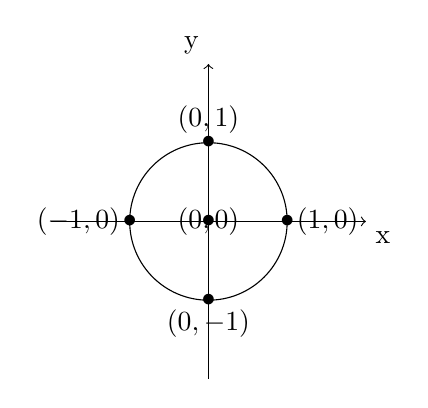
\begin{tikzpicture}
	\pgfmathsetmacro\MAX{2}
	\draw[->] (-\MAX,0) -- (\MAX,0) node[anchor=north west] {x};
	\draw[->] (0,-\MAX) -- (0,\MAX) node[anchor=south east] {y};
	\draw node at (0,0) {$(0,0)$};
	\draw node at (0,0) {$\bullet$};
	\draw node at (0,1) {$\bullet$};
	\draw node at (0,1) [anchor=south]{$(0,1)$};
	\draw node at (1,0) {$\bullet$};
	\draw node at (1,0) [anchor=west] {$(1,0)$};
	\draw node at (-1,0) {$\bullet$};
	\draw node at (-1,0) [anchor=east] {$(-1,0)$};
	\draw node at (0,-1) {$\bullet$};
	\draw node at (0,-1) [anchor=north]{$(0,-1)$};
	\draw (0,0) circle (1);
	\end{tikzpicture}\\
	Per prima cosa osservo che s possono trovare dei punti che rendono vera $f(x,y)=x^2+y^2-1=0$ e sono tutti i punti della circonferenza di centro l'origine degli assi e raggio unitario.\\
	il punto $(x_0,y_0)=(0,1)$ definisce implicitamente una funzione $y=\varphi(x)=\sqrt{1-x^2}$ con $\mathcal{X}=[-1,1]$ e $\mathcal{Y}=[0,1]$\\
	un primo problema è dovuto alla scelta degli intervalli $\mathcal{X},\mathcal{Y}$, per esempio posso scegliere $\mathcal{X}=[-\frac{1}{2},\frac{1}{2}]$ e $\mathcal{Y}=R^+$\\
	un secondo problema è la scelta del punto $(x_0,y_0)$, potrei scegliere il punto $(\frac{1}{\sqrt{2}},\frac{1}{\sqrt{2}})$\\
\observation
La stessa definizione può essere riscritta con la $x$ funzione della $y$ poiché a priori non c'è distinzione tra le variabili.
\proposition (caso lineare)\\
sia $f:R^n\times \R^m\rightarrow \R^p$ che $(x,y)\rightarrow Ax+By-C$ con $A\in Mat(p \times n), B\in (p \times m), B\in (p \times 1)$. Se $p=m$ cioè $B$ è un matrice quadrata, e $det(B)\ne 0$ cioè invertibile, allora\\
$\exists !\varphi : \R^n\rightarrow \R^m$ t.c.: $f(x,y)=0 \Leftrightarrow y=\varphi(x)$
\begin{proof}
	$f(x,y)=0\Leftrightarrow Ax+By=-C\Leftrightarrow By=-Ax+C\Leftrightarrow y=-B^{-1}Ax+B^{-1}C = \varphi(x)$
\end{proof}
\begin{theorem}[Teorema della Funzione Implicita]
	\label{teo:funz_impl}
	Sia $f:X\times Y\rightarrow \R^m$ con $X\subseteq \R^n, Y\subseteq \R^m$\\
	Preso un punto $(x_0,y_0)$ con $x_0\in \circdot{X}$,$y_0\in \circdot{Y}$\\
	se:
	\begin{enumerate}
		\item $f$ continua in $X\times Y$
		\item $f(x_0,y_0)=0$
		\item $f$ differenziabile rispetto a $y \forall (x,y)\in X\times Y$ e $D_yf(x,y)$ continua.
		\item $D_yf(x_0,y_0)$ invertibile .
	\end{enumerate}
	$\Rightarrow $ si ha:\\
	esistenza della funzione implicita\\
	$\exists \mathcal{X}\subseteq X$ intorno di $x_0$(xstrano aperto)\\
	$\exists \mathcal{Y}\subseteq Y$ intorno di $y_0$(ystrano aperto)\\
	$\exists\varphi$ continua con $\varphi:\mathcal{X}\rightarrow\mathcal{Y}$ t.c. $[\varphi (x_0)=y_0 e] f(x,y)=0, x\in\mathcal{X},y\in\mathcal{Y} \Leftrightarrow y=\varphi(x)$
	unicità di sostanza cioè a meno del dominio:\\
	se $\varphi_i:\mathcal{X}_i\rightarrow\mathcal{Y}_i$ e $x_0\in\mathcal{X}_i,y_0\in\mathcal{Y}_i$\\
	$f(x_0,y_0)=0 \forall x\in\mathcal{X}_i, y\in \mathcal{Y}\Leftrightarrow y=\varphi_i(x)$ con $i=1,2$\\
	Allora $\forall\in\mathcal{X}\cap\mathcal{X}_1\cap\mathcal{X}_2$ vale $\varphi_1(x)=\varphi_2(x)$

	\observation
	Le ipotesi 3 e 4 garantiscono che esiste una approssimazione lineare, l'ipotesi 4 è sensata poiché $y$ e $f$ hanno lo stesso numero di componenti quindi $Dyf$ è un matrice qudrata.\\
	la funzione $f:X\times Y\rightarrow \R^m$ che $(x,y)\rightarrow f(x,y)$ ??????\\
	cioè $\forall x\in X$ (sto fissando una x) $f^x:Y\rightarrow \R^m$ che $y\rightarrow f(x,y)$(sto variando la y), $Df^x\in Mat(m\times m)$

	\observation Metodo degli zeri di Newton per troare gli zeri di una funzione o metofo delle tangenti.\\
	\resizebox {\columnwidth} {!} {
	\begin{tikzpicture}
	\draw[->] (-1,0) -- (5,0) node[anchor=north west] {y};
	\draw[->] (0,-1) -- (0,4) node[anchor=south east] {z};
	\draw[domain=-1:4,smooth,variable=\x,blue] plot ({\x},{(1/8)*(\x*\x)-(\x)+1.9});
	\end{tikzpicture}
	}\\
	Scelgo un punto $y_0$ ne prendo il valore sulla curva, disegno la tangente e chiamo $y_1$ l'intersezione con l'asse $y$. Itero il processo $y_n+1=y_n\frac{f(y_n)}{f'(y_n)}$\\
	discorso al momento difficile per me....\\
	\begin{proof}
		Dobbiamo partire da $f(x,y)=0$ arrivare a $y=\varphi(x)$,vogliamo applicare un raginamento simile a quello della Metodo di Newton, passando però per il concetto di punto fisso, il teorema delle Contrazioni ci assicura che esiste unico.\\
		cerchiamo quindi una contrazione $T$ il cui punto fisso sia soluzione di $f(x,y)=0$. $T$ è del tipo:\\
		$T:?\times ?\rightarrow ?$\\
		$(x,y)\rightarrow y-[D_yf(X_0,y_0)]^{-1}f(x,y)$, nota che non avere nella derivata lo stesso punto in cui si calcola la funzione (come è nel metodo di Newton) ha effetti "tragici" sulla velocità di convergenza, ma a noi interessa l'esistenza.\\
		bisgna capire quali insiemi usare come insiemi di partenza e arrivo, devo essere scelti in modo da poter applicare il teoremma delle contrazioni. Bisogna scegliere sottoinsiemi di $R^n$ e $R^m$, scegliamo quindi delle sfere\\
		$T:\overline{B(x_0,r_x)}\times\overline{B(y_0,r_y)}\rightarrow\overline{B(y_0,r_y)}$, scegliendo la chiusura delle sfere si è sicuri di lavorare in uno spazio metrico completo, poiché in $R^l$ completo $\Leftrightarrow$ chiuso e limitato.\\
		come vengono invece scelti i raggi? sono scelti in modo che:\\
		\begin{enumerate}
			\item $T$ è ben definita
			\item $\forall x \in \overline{B(x_0,r_x)} Tx: \overline{B(x_0,r_x)}\rightarrow\overline{B(y_0,r_y)}$ che $y\rightarrow T(x,y)$,\\
		\end{enumerate}
		cioè $T$ è una contrazione tale che $\forall x$ esiste un punto fisso, $\forall x$ associo a $y$ una x, e quindi na funzione.\\
		$r_x,r_y$ devono essere sufficientemene piccoli per avere tali proprietà e per poterci lavorare sopra.\\
		Abbiamo che $f(x,y)=0 \Leftrightarrow T(x,y)=y$\\
		$T(x,y)=y\Leftrightarrow y=y-[D_yF(x_0,y_0)]^{-1}f(x,y)$\\
		$[D_yF(x_0,y_0)]^{-1}f(x,y)\Leftrightarrow f(x,y)=0$\\
		Per verificare che $T$ è una contrazione ne stimo la norma\\
		$\norm{T(x,y_2)-T(x,y_1)} \le \sup\limits_{\widetilde{y}\in segmento}\norm{D_yT(x,\widetilde{y})}\norm{y_2-y_1} $  accrescimenti finiti.\\
		Poichè le sfere sono insiemi convessi è stato possibile applicare il Teorema degli accresscimenti finiti.\\
		Presa $T(x,y) = y-[D_yf(x_0,y_0)]^{-1}f(x,y)$, la derivo rispetto a $y$:
		$$D_yT(x,y)= I_\R^m-[D_yf(x_0,y_0)]^{-1}D_yf(x,y) = $$
		$$=[D_yf(x_0,y_0)]^{-1}][D_yf(x_0,y_0)-D_yf(x,y)]$$
		Osserviamo che abbiamo ottenuto una matrice come costante moltiplicativa, al secondo membro abbiamo la differenza di due valori di una funzione, che per ipotesi è una funzione continua ($D_yf(x,y)$ continua), allora per $r_x$ e $r_y$ sufficientemente piccoli ho che:\\
		$\norm{D_yT(x,y)} \le \frac{1}{2}$, è scelto questo valore poiché è comodo al fine di dimostrare la contrazione...\\
		$$\norm{D_yT(x,y)} \le \norm{D_yf(x_0,y_0)]^{-1}} \norm{D_yf(x_0,y_0)-D_yf(x,y)}\le\frac{1}{2} $$  
		$$\norm{T(x,y_2)-T(x,y_1)}\le\frac{1}{2}\norm{y_2-y_1} $$
		Se dimostriamo che $T$ è ben definita abbiamo dimostrato che $T$ è una contrazione.\\
		Per verificare che $T$ è en definita bisogna mostrare che $T(x,y)\subseteq\overline{B(y_0,r_y)}$ quindi si mostra che la distanza tra $T(x,y)$ e il centro è minore di $r_y$
		$$\norm{T(x,y) - y_0}\le\norm{T(x,y)-T(x,y_0)}+\norm{T(x,y_0)-y_0} \le$$
		$$\le\frac{1}{2}\norm{y-y_0}+\norm{y_0-[D_yf(x_0,y_0)]^{-1}f(x,y_0)-y_0}\le$$
		$$\le\frac{1}{2}\norm{y-y_0}+\norm{[D_yf(x_0,y_0)]^{-1}} \norm{f(x,y_0)-0}\le$$
		$$\le\frac{1}{2}\norm{y-y_0}+\norm{[D_yf(x_0,y_0)]^{-1}} \norm{f(x,y_0)-f(x_0,y_0)}\le$$
		$$\le\frac{1}{2}r_y+\frac{1}{2}r_y\le r_y$$
		Allora $T$ è ben definita perché $T(x,y)\in\overline{B(y_0,r_y)}$.\\
		In conclusione con $\mathcal{X}=\overline{B(x_0,r_x)}$ e $\mathcal{Y}=\overline{B(y_0,r_y)}$ ho che $T:\mathcal{X}\times\mathcal{Y}\rightarrow\mathcal{Y}$ è tale che $\forall x\in\mathcal{X}$ la funzione $y\rightarrow T(x,y)$ è una contrazione e $\overline{B(y_0,r_y)}$ è completo.\\
		quaolcosa sui completi.........\\
		................................\\
		..........................\\
		A questo punto può essere applicato il teorema delle contrazioni:\\
		$\forall x \in \mathcal{X}, \exists y \in\mathcal{Y}: f(x,y)=0$ allora chiamo $\varphi:\mathcal{X}\rightarrow\mathcal{Y}$ che $x\rightarrow y$ è unica quindi $\varphi$ è una funzione.\\
		Allora la funzione implicita esiste. La continuità direva direttamente dal teorema delle contrazioni: l'applicazione che al parametro associa il punto fisso è continua.\\
		Per l'unicità si osservano le ipotesi 1 e 2, dove è scritto $\forall x$ ovvero scelta una qualunque $x$ la $y$ è unica quindi $\varphi$ è univocamente definita.
		
	\end{proof}
\end{theorem}
\proposition
Sia $f:X\times Y\rightarrow \R^m$ con $X\in \R^n, Y\in \R^m$\\
Preso un punto $(x_0,y_0)$ con $x_0\in \circdot{X}$,$y_0\in \circdot{Y}$\\
se:
\begin{enumerate}
	\item $f(x_0,y_0)=0$
	\item $f\in \cntclass{1}(X\times Y,R^m)$.
	\item $D_yf(x_0,y_0)$ invertibile .
\end{enumerate}
$\Rightarrow $ si ha:\\
\begin{enumerate}
	\item $\exists \varphi: \mathcal{X}\rightarrow\mathcal{Y}$ definita implicitamente da $f(x_0,y_0)=0$
	\item $\varphi$ continua su $\mathcal{X}$
	\item $\varphi$ è differenziabile e $D\varphi(x)=-[D_yf(x,\varphi(x))]^{-1}D_xf(x,\varphi(x))$
\end{enumerate}
\begin{proof}
	I punti 1 e 2 sono gli stessi del teorema della funzione implicita e si dimostrano allo stesso modo.\\
	Per il punto 3 abbiamo che $f(x,y)=0\Leftrightarrow y=\varphi(x)$ e quindi $\forall x\in \mathcal{X}$ $f(x,\varphi(x))=0$\\
	.........\\
	.........\\
	
\end{proof}

\proposition CASO N=1, M=1\\
Sia $f:X\times Y\rightarrow \R$ con $X\in \R, Y\in \R$\\
Preso un punto $(x_0,y_0)$ con $x_0\in \circdot{X}$,$y_0\in \circdot{Y}$\\
se:
\begin{enumerate}
	\item $f(x_0,y_0)=0$
	\item $f\in \cntclass{1}(X\times Y,R)$.
	\item $\partial_yf(x_0,y_0)\ne 0$.
\end{enumerate}
$\Rightarrow $ si ha:\\
\begin{enumerate}
	\item $\exists \varphi: \mathcal{X}\rightarrow\mathcal{Y}$ definita implicitamente da $f(x_0,y_0)=0$
	\item $\varphi\in \cntclass{0}(\mathcal{X},\mathcal{Y})$
	\item $\varphi$ è derivabile e $\varphi'(x)=-[\partial_yf(x,\varphi(x))]^{-1}\partial_xf(x,\varphi(x))$
\end{enumerate}
\begin{proof}
	$f(x,y)=0\Leftrightarrow y=\varphi(x)$, derivando $D(f(x,\varphi(x)))=0$\\
	$\partial_xf(x,\varphi(x))+\partial_yf(x,\varphi(x))\varphi'(x)=0$\\
	allora $\varphi'(x) = -\frac{\partial_xf(x,\varphi(x))}{\partial_yf(x,\varphi(x))}$
\end{proof}
\observation Non essendoci motivo per preferire la $x$ alla $y$ o viceversa, esiste anche una versione di questo teorema  in  cui le ipotesi sono le stesse eccetto l'ultima che diventa $\partial_xf(x_0,y_0)\ne 0$
\begin{enumerate}
	\item $\exists \psi: \mathcal{Y}\rightarrow\mathcal{X}$ definita implicitamente da $f(x,y)=0$
	\item $\psi\in \cntclass{0}(\mathcal{Y},\mathcal{X})$
	\item $\psi$ è derivabile e $\psi'(y)=-[\partial_xf(\psi(y),y)]^{-1}\partial_yf(\psi(y),y)$
\end{enumerate}
Qualche esempio qui\\
\subsection{Il Teorema della funzione Inversa}
Data una funzione f, poterla invertire  ...... unico modo l'equazione (o sistema ....)... l'incognita $x$ in funzione del parametro .....\\
\proposition(Teorema della funzione inversa caso lineare)\\
Sia $f:R^n\in \R^m$ data da $f(x)=Mx$ e $M\in Mat(m\times n)$, $f$ è invertibile $\Leftrightarrow n=m$ e $detM\ne 0$
\proposition(caso generale)\\
sia $f:A\rightarrow \R^n$ con $A\in \R^n$, $f\in \cntclass{1}(A,R^n)$, $x_0\in \circdot{A}$ e $Df(x_0)$ invertibile.\\
Allora $\exists\mathcal{X}\in A,\exists\mathcal{Y}\in \R^n$, $\exists\varphi\mathcal{Y}\rightarrow\mathcal{X}$ con la proprietà $f(x)=y\Leftrightarrow x=\varphi(y)$ con $x\in\circdot{\mathcal{X}}$ e $y\in\circdot{\mathcal{Y}}$ e $\varphi\in \cntclass{1}(\mathcal{Y},\mathcal{X})$ e $D\varphi(y)=[Df(x)]^{-1}$\\
\begin{proof}
	$f(x)=y\Leftrightarrow f(x)-y=0$. Allora introduco $F:A\times \R^n\rightarrow \R^n$ data da $F(x,y)=f(x)-y$.\\
	Studio $F(x,y)=0$ per ottenere $x=\varphi(y)$.\\
	Per poter applicare il teorema della funzione implicita serve $D_xF(x_0,y_0)$ invertibile, ma $D_xF(x_0,y_0)=Df(x_0)$ che è invertibile per ipotesi.\\
	Applico allora il teorema della funzione implicita , quindi gli intorni esistono e $x=\varphi(y)$.\\
	resta da trovare la derivata totale di $\varphi$. Sappiamo che $f\in \cntclass{1}$ quindi $\varphi \in \cntclass{1}$.\\
	Sappiamo che $\varphi(f(x))=x$, applicando la derivata della funzione composta abbiamo che:\\
	$D\varphi(f(x))Df(x)=I$\\
	$D\varphi=[Df(x)]^{-1}$ quando $\varphi(y)=x$\\
	si puo anche scrivere come $(Df^{-1})(f(x))=[Df(x)]^{-1}$
\end{proof}
\section{Massimi e Minimi Liberi}
\definition
Siano $(X,d)$s.m., $A\subseteq X$ e $f:A\rightarrow \R$, siano $x_0\in A, B\in A$ e $m,M\in \R$ ( L'insieme immagini deve essere $R$ per poter parlare di massimi e minimi, $R$ è un campo ordinato a differenza di $R^n$).\\
$M$ è massimo di $f$ su $B \rightleftharpoons M=\max f(B)\Leftrightarrow\forall x \in B f(x_0)\ge f(x)$\\
$M$ è minimo di $f$ su $B \rightleftharpoons m=\min f(B)\Leftrightarrow\forall x \in B f(x_0)\le f(x)$\\
$x_0$ è punto di massimo assoluto per $f \rightleftharpoons f(x_0)=\max\limits_{A}f(x)$\\
$x_0$ è punto di minimo assoluto per $f \rightleftharpoons f(x_0)=\min\limits_{A}f(x)$\\
$x_0$ è punto di massimo locale relativo per $f \rightleftharpoons \exists r>0: f(x_0)=\max\limits_{x\in B(x_0,r)}f(x)$ con $B(x_0,r)\subseteq A$\\
$x_0$ è punto di minimo locale relativo per $f \rightleftharpoons \exists r>0: f(x_0)=\min\limits_{x\in B(x_0,r)}f(x)$ con $B(x_0,r)\subseteq A$\\
\subsection{Condizioni Necessarie}
\proposition{Teorema di Fermat}\\
sia $f:A\subseteq \R^n\rightarrow \R$ e $x_0\in\circdot{A}$. Se $x_0$ è punto di massimo(0 minimo) locale per $f$ su $A$ e $f$ è differenziabile in $x_0$ allora $\nabla f(x_0)=0$.
\begin{proof}
	Sia $v\in \R^n$ con $\norm{v} =1$, la funzione $F(t)= f(x_0+tv)$ che a $t\rightarrow x_0+tv$ è il moto rettilineo uniforme che passa da $x_0$ all'istante $0$ e si muove con velocità vettore costante $v$. cioè per tempi negativi mi avvicino a $x_0$ al tempo zero si è in $x_0$ e per tempi positivi si allontana da $x_0$. quindi $t=0$ è punto di massimo per $F$, allora $F'(0) = 0$ per il teorema di Fermat di A1.\\
	Ora abbiamo che $F'(t)=\nabla f(x_0+tv)v$ quindi $F'(0)=\nabla f(x_0)v$ cioè $\nabla f(x_0)v=0$.\\
	Quindi $\forall v :\norm{v} =1$ vale $\nabla f(x_0)=0$\\
	OSS:: Vale anche che $D_vf(x_0)=0$
\end{proof}
\definition
sia $f:A\subseteq r^n\rightarrow \R$, $x_0\in\circdot{A}$\\
$x_0$ è punto stazionario .... $\rightleftharpoons$ $f$ è differenziabile in $x_0$ e $\nabla f($ ......
\observation
nel caso $n=2, m=1, \nabla f(x_0,y_0)=[\partial_xf(x_0,y_0), \partial_yf(x_0,y_0)]$ ..... i punti stazionari sono quelli che ......parziali.
\observation
Prima di continuare un paio di osservazioni sulle forme quadratiche.\\
\definition
forma quadratica su $R^n \rightleftharpoons q:R^n\rightarrow \R$ che $x\rightarrow x^TQx$ con $Q\in Mat(n\times n)$ simmetrica\\
ESEMPI:n=2\\
$$
Q=\begin{bmatrix}1&&0\\0&&1\end{bmatrix}\quad
Q=\begin{bmatrix}-1&&0\\0&&-1\end{bmatrix}\quad
Q=\begin{bmatrix}-1&&0\\0&&1\end{bmatrix}\quad 
$$
SEMPRE POSITIVA SEMPRE NEGATIVA CAMBIA SEGNO\\
SEMPRE POSITIVA SEMPRE NEGATIVA CAMBIA SEGNO\\
SEMPRE POSITIVA SEMPRE NEGATIVA CAMBIA SEGNO\\
\proposition
se $Q$ è una forma quadratica, allora\\
\begin{itemize}
	\item $\forall\lambda\in \R, \forall x\in \R^n$ $q(\lambda x)=\lambda^2q(x)$
	\item $q(0)=0$
	\item se $q$ è limitata $\Rightarrow q\equiv 0$ 
\end{itemize}
\begin{proof}
	\begin{itemize}
		\item $q(\lambda x)=(\lambda x)^TQ(\lambda x)=\lambda^2x^TQx=\lambda^2q(x)$
		\item $q(0)=q(0x)=0q(x)=0$
		\item (contronominale $q\ne 0 \Rightarrow q$ non è limitata).\\
		se $q$ è non nulla $\Rightarrow \exists x \in \R^n$ $q(x)\ne 0$\\
		allora $q(\lambda x)=\lambda^2q(x)$ illimitata.
		\item ???????????????????????????????????????????????
	\end{itemize}
\end{proof}
\proposition
se $q$ è una forma quadratica $\Rightarrow\exists M\ge 0: \abs{q(x)}\le M\norm{x}^2$ $\forall x\in \R^n$
\begin{proof}
	per $x\ne 0$ $\abs{q(x)} =\abs{q\left(\norm{x} \frac{1}{\norm{x} }x\right)} = \norm{x}^2\abs{q\left(\frac{1}{\norm{x}}x\right)}\le$\\
	$\le\left(\sup\limits_{\norm{x}=1}\abs{q(x)}\right)\norm{x}^2=\le\left(\max\limits_{\norm{x}=1}\abs{q(x)}\right)\norm{x}^2=M\norm{x}^2$
\end{proof}
\proposition
Sia $q$ una forma quadratica, se $q(x)=o(\norm{x}^2)$ per $x\rightarrow 0 \Rightarrow q\equiv 0$
\begin{proof}
	sia $x\in \R^n$ con $\norm{x}=1$ e $t>0$.\\
	$q(x)=\frac{1}{t^2}$, $q(tx)=\frac{q(tx)}{\norm{tx}^2}\rightarrow 0$ per $t\rightarrow 0$ per ipotesi.\\
	Allora $\forall x$ con $\norm{x}$ vale $q(x)=0$ e allora $\forall x\ne 0, q(x)=q\left(\frac{1}{\norm{x}}x\right)\norm{x}^2$
\end{proof}
\definition
Sia $q:R^n\rightarrow \R$ una forma quadratica\\
\begin{itemize}
	\item $q$ è definita positiva $\rightleftharpoons \forall x\in \R^n, x\ne 0$ $q(x)>0 [Q>0]$
	\item $q$ è semidefinita positiva $\rightleftharpoons \forall x\in \R^n$ $q(x)\ge0 [Q\ge0]$
	\item $q$ è definita negativa $\rightleftharpoons \forall x\in \R^n, x\ne 0$ $q(x)<0 [Q><0]$
	\item $q$ è semidefinita negativa $\rightleftharpoons \forall x\in \R^n$ $q(x)\le0 [Q\le0]$
\end{itemize}
\proposition
Sia $q:R^n\rightarrow \R$ una forma quadratica, se $q$ è definita positiva $\Rightarrow \exists m>0: \forall x \in \R^n, q(x)\ge m\norm{x}^2$
\begin{proof}
	Noto che $q(\lambda x)=\lambda^2q(x)$\\
	$q(x)=q\left(\frac{1}{\norm{x}}x\norm{x}^2\right)\ge\min\limits_{\norm{x}=1}q(\lambda)\norm{x}^2$
\end{proof}
Ora dobbiamo cercare di capire se $q$ è definita positiva\\
Ad esempio: $Q=\begin{bmatrix}1&&0&&0\\0&&-1&&0\\0&&0&&0\end{bmatrix}$ è facile capire che è semodefinita positiva poiché è in diagonale, quindi la prima cosa da fare è trovare una forma diagonale per $Q$\\
un procedimento pratico e veloce è il seguente:\\
$$Q=\begin{bmatrix}q_{11}&&q_{12}&&q_{13}&&\ldots\\q_{21}&&q_{22}&&q_{23}&&\ldots\\q_{31}&&q_{32}&&q_{33}&&\ldots\\\vdots&&\vdots&&\vdots&&\ddots\end{bmatrix}\rightarrow\begin{bmatrix}\lambda_{1}&&0&&0&&\ldots\\0&&\lambda_{2}&&0&&\ldots\\0&&0&&\lambda_{3}&&\ldots\\\vdots&&\vdots&&\vdots&&\ddots\end{bmatrix}$$
$$\lambda=q_{11},\quad\lambda_{2}=\frac{detQ_2}{q_11}\quad\lambda_{3}=\frac{detQ_3}{detQ_2}\quad ...\quad \lambda_{i}=\frac{detQ_i}{detQ_{i-1}}$$
Questo perché se dobbiamo valutare il segno dell'incremento della f ci servono le variazioni sulle quadriche. Se $f$ è $\cntclass{2}$ scrivo lo sviluppo di Taylor al secondo ordine:\\
$$f(x)-f(x_0)=\nabla f(x_0)(x-x_0)+\frac{1}{2}(x-x_0)^TH_f(x_0)(x-x_0)+o(\norm{x-x_0}^2)$$
max e min dove $\nabla f(x_0)=0$ per Fermat, l'o piccolo è trascurabile, allora il segno della derivata dipende dalla forma quadratica al secondo membro.
\proposition
sia $f:A\subseteq \R^n\rightarrow \R$ e $x_0\in\circdot{A}$.\\
$f\in \cntclass{2}(A;R)$ e $x_0$ punto di massimo locale per $f$ su $A\Rightarrow\nabla f(x_0)=0$ e $H_f(x_0)$ è semidefinita negativa.
\begin{proof}
	$f(x)-f(x_0)=\frac{1}{2}(x-x_0)^TH_f(x_0)(x-x_0)+o(\norm{x-x_0}^2)$ poiché $f\in \cntclass{2}$\\
	il primo termine è negativo poiché per ipotesi $x_0$ è punto di massimo locale, ne segue che il termine $(x-x_0)^TH_f(x_0)(x-x_0)$ non può essere positivo. 
\end{proof} 
\proposition
sia $f:A\subseteq \R^n\rightarrow \R$ e $x_0\in\circdot{A}$.\\
$f\in \cntclass{2}(A;R)$ e $x_0$ punto di minimo locale per $f$ su $A\Rightarrow\nabla f(x_0)=0$ e $H_f(x_0)$ è semidefinita positiva.
\begin{proof}
	$f(x)-f(x_0)=\frac{1}{2}(x-x_0)^TH_f(x-x_0)+o(\norm{x-x_0}^2)$ poiché $f\in \cntclass{2}$\\
	il primo termine è positivo poiché per ipotesi $x_0$ è punto di minimo locale, ne segue che il termine $(x-x_0)^TH_f(x-x_0)$ non può essere negativo. 
\end{proof} 


\subsection{Condizioni Sufficienti}
\proposition
sia $f:A\subseteq \R^n\rightarrow \R$ e $x_0\in\circdot{A}$.\\
$f\in \cntclass{2}(A;R)$, $\nabla f(x_0)=0$,$H_f(X_0)$ è definita negativa $\Rightarrow x_0$ è un punto di massimo locale per $f$
\begin{proof}
	$f\in \cntclass{2}$ quindi possiamo scrivere:\\
	$f(x_+h)-f(x_0)=\nabla f(x_0)h+\frac{1}{2}(h)^TH_f(x_0)+o(\norm{h}^2)$ per $h\rightarrow 0$\\
	$f(x_+h)-f(x_0)=\frac{1}{2}(h)^TH_f(x_0)+o(\norm{h}^2)$ per $h\rightarrow 0$\\
	Sappiamo che $H_f$ è definita negativa per ipotesi, allora $h^TH_f(x_0)h\le -m\norm{x_0}$ allora $f(x_0+h)-f(x_0)<0$ e quindi $x_0$ è punto di massimo locale per $f$.
\end{proof} 
\proposition
sia $f:A\subseteq \R^n\rightarrow \R$ e $x_0\in\circdot{A}$.\\
$f\in \cntclass{2}(A;R)$, $\nabla f(x_0)=0$,$H_f(X_0)$ è definita positiva $\Rightarrow x_0$ è un punto di minimo locale per $f$
\begin{proof}
	$f\in \cntclass{2}$ quindi possiamo scrivere:\\
	$f(x_+h)-f(x_0)=\nabla f(x_0)h+\frac{1}{2}(h)^TH_f(x_0)+o(\norm{h}^2)$ per $h\rightarrow 0$\\
	...........\\
	...........\\
\end{proof} 
QUALCHE DISEGNO E SPIEGAZIONE.....
\subsection{Il Significato Geometrico del Gradiente n=2 m=1}
\definition
Sia $A\subseteq \R^2$ e $f:A\rightarrow \R$\\
La suferficie $z=f(x,y)$ è il grafico di $f$, è unsottoinsieme di $R^3$\\
Se $c\in \R$, la curva di livello $c$ di $f$ è l'insieme $f^{-1}(c)\{(x,y)\in A: f(x,y)=c\}$\\
Se $f$ 	'e differenziabile in $(x_0,y_0)\in\circdot{A}$ il piano tangente alla superficie $z=f(x,y)$ in $(x_0,y_0)$ ha equazione:\\
$$z=f(x_0,y_0)+\nabla f(x_0,y_0)\begin{bmatrix}(x-x0)\\(y-y_0)\end{bmatrix}$$ 
$$z=f(x_0,y_0)+\partial_xf(x_0,y_0)(x-x_0)+\partial_yf(x_0,y_0)(y-y_0)$$
\observation
geometricamente, il gradiente di una funzione indica la direzione di $R^n$ in cui si ha la massima variazione del valore di f, nel verso di incremento positivo di $f$,
\observation 
osservazione col grafico che al momento non faccio.
\proposition
Siano $A\subseteq \R^n, f:A\rightarrow \R$ differenziabile in $(x_0,y_0)\in \circdot{A}$, l'incremento di $f(x_0+h,y_0+k)-f(x_0,y_0)$ è massimo quando $[h k]=\lambda\nabla f(x_0,y_0)$ con $\lambda >0$ ed è minimo con $[h k]=\lambda\nabla f(x_0,y_0)$ con $\lambda <0$
\begin{proof}
	so che posso approssimare la funzione quindi posso scrivere:\\
	$f(x_0+h,y_0+k)-f(x_0,y_0)=\nabla f(x_0,y_0)\begin{bmatrix}h\\k\end{bmatrix}+o(\sqrt{h^2+k^2})$=
	$=\norm{\nabla f(x_0,y_0)}\norm{\begin{bmatrix}h k\end{bmatrix}}cos(\theta)+o(\sqrt{h^2+k^2})$\\
	dove $\theta$ è l'angolo tra $\nabla f(x_0,y_0)$ e $[h k]$ per $||[h k]||$ sufficientemente piccola, l'incremento $f(x_0+h,y_0+k)-f(x_0,y_0)$ è massimo se $cos( \theta )=1$ ed è minimo se $cos(\theta )=-1$, da cui la tesi.\\ 
\end{proof}
\proposition
siano $f\in \cntclass{1}(A;R)$ con $A\subseteq \R^2$ e $(x_0,y_0)\in\circdot{A}$ e $\nabla f(x_0,y_0)\ne 0$[cioè stazionario]. Allora $nabla f(x_0,y_0)$ è perpendicolare alla curva di livello passante per .....
\observation
un vettore 1'e perpendicolare a una curva se è perpendicolare alla retta o al vettore tangente alla curva in quel punto.
\begin{proof}
	La curva di livello è $f(x,y)=f(x_0,y_0)$ cioè $f(x,y)-f(x_0,y_0)=0$, per trovare la tangente a questa curva è piu facile se si ha $y=\varphi(x)$\\
	Usiamo quindi il teorema della funzione implicita, mi serve che $\partial_yf(x_0,y_0)\ne 0$, questa condizione non è assicurata dalle ipotesi, per ipotesi il gradiente è non nulla quindi almeno una delle due componenti è non nulla.\\
	Inizio con il caso $\partial_yf(x_0,y_0)\ne 0$.\\
	Il T.F.IMPL. assicura che :\\
	$\exists\mathcal{X},\mathcal{Y}$ con $x_0\in\circdot{\mathcal{X}}, y_0\in\circdot{\mathcal{Y}}$, $\exists\varphi:\mathcal{X}\rightarrow\mathcal{Y}$ t.c.:\\
	$f(x,y)=f(x_0,y_0), x\in\mathcal{X}, y\in\mathcal{Y} \Leftrightarrow y=\varphi(x)$\\
	La retta tangente in $x_0$ a $y=\varphi(x)$ è $y=y_0+\varphi'(x_0)(x-x_0)$\\
	questo vuole dire che un vettore tangente a $y=\varphi(x)$ in $(x_0,y_0)$ è $\begin{bmatrix}1\\\varphi'(x_0)\end{bmatrix}$.\\
	... calcolo il prodotto scalare\\
	$$\nabla f(x_0,y_0)\begin{bmatrix}1\\\varphi'(x_0)\end{bmatrix} = \begin{bmatrix}\partial_x f(x_0,y_0)&&\partial_y f(x_0,y_0)\end{bmatrix}\begin{bmatrix}1\\-\frac{\partial_x f(x_0,y_0)}{\partial_y f(x_0,y_0)}\end{bmatrix} =$$ 
	$$=\partial_x f(x_0,y_0) -\partial_y f(x_0,y_0)\frac{\partial_x f(x_0,y_0)}{\partial_y f(x_0,y_0)}=0$$
	Allora il graadiente è perpendicolare alla curva di livello.\\
	Guardiamo ora al caso in cui $\partial_yf(x_0,y_0)= 0$ e $\partial_xf(x_0,y_0)\ne 0$ quindi il gradiente è non nullo.\\
	Applicando lo stesso ragionamento id sopra, solo esplicitando la $x$ in funzione della $y$. Quindi $x=\psi(x)$ e $\psi{'}(y_0)=-\frac{\partial_y f(x_0,y_0)}{\partial_x f(x_0,y_0)}$
\end{proof}

\section{Massimi e Minimi Vincolati}
Spesso la ricerca di punti di massimo o minimo di una funzione $f:A\rightarrow \R, A\subseteq \R^n$ deve essere ristrettaad un sottoinsieme $B\subseteq A$ a causa di eventuali vincoli a cui le variabili indipendenti devono soddisfare. L0insieme $B$ può essere generalmente descritto da una funzione $\varphi :A\rightarrow \R^p$, nel senso che $B=\{x\in A:\varphi (x)\le 0\}$\\
NOTA::: direi n>1 poiché se ho una sola variabile e la vincolo ...??????? booooo .\\
Questo problema è usualmente abbreviato in:
$$\max\limits_{\varphi \le 0}\quad o \quad\min\limits_{\varphi \le 0}$$
può essere affrontato in due passi:\\
\begin{enumerate}
	\item ricerca dei punti di estremo di $f$ interni a $B$, problema gia affrontato.
	\item ricerca dei punti di estremo di $f$ sul bordo di $B$, affrontiamo ora.
\end{enumerate}
Sotto opportune condizioni su $\varphi$, infatti, $\circdot{B} = \{x\in A:\varphi(x)<0\}$ e $\partial B\{x\in A:\varphi(x)=0\}$
\proposition{Teorema dei Moltiplicatori di Lagrange}
Siano $f,g:A\subseteq \R^2\rightarrow \R, (x_0,y_0)\in\circdot{A}, g(x_0,y_0)=0, f,g\in \cntclass{1}(A;R)$, $\nabla g (x_0,y_0)\ne 0$\\
Se $(x_0,y_0)$ è di max(o min) locale per $f$ su $g=0\Rightarrow\exists \lambda in \R$ t.c: $\nabla f(x_0,y_0) = \lambda g(x_0,y_0)$ (all fin fine posso dire che sono paralleli).\\
\observation
$\lambda$ si chiama "moltiplicatore di lagrange"
\observation
Se abbiamo un problema del tipo $\max\limits_{g(x,y)=0}f$ cioè il massimo di $f$ sul vincolo $g(x,y)=0$, ci dobbiamo ricondurre ad un sistema del tipo
$\begin{cases} \nabla f(x_0,y_0)=\lambda \nabla g(x_0,y_0)\\ g(x_0,y_0)=0 \end{cases}=\begin{cases} \partial_xf(x_0,y_0)=\lambda \partial_xg(x_0,y_0)\\\partial_yf(x_0,y_0)=\lambda \partial_yg(x_0,y_0)\\ g(x_0,y_0)=0 \end{cases}$\\
3 equazioni in 3 incognite($x,y,\lambda$)\\
In certi casi si introduce una funzione $\mathcal{L}(x,y,\lambda) = f(x,y)-\lambda g(x,y)$ detta Lagrangiana, i punti stazionari vincolati di $f$ sono punti stazonari liberi della Lagrangiana.\\
\begin{proof}
	Sappiamo che $\nabla g(x_0,y_0)\ne$ quindi $\begin{bmatrix}\partial_xg(x_0,y_0) &&\partial_yg(x_0,y_0)\end{bmatrix}\ne\begin{bmatrix}0&&0\end{bmatrix}$ quindi o $\partial_xg(x_0,y_0)\ne 0$ o $\partial_yg(x_0,y_0)\ne 0$.
	Mettiamoci nel caso in cui $\partial_yg(x_0,y_0)\ne 0$,\\
    Per il teorema della funzione implicita ho che :\\
	$\exists\mathcal{X},\mathcal{Y}$ con $x_0\in\circdot{\mathcal{X}}, y_0\in\circdot{\mathcal{Y}}$, $\exists\varphi:\mathcal{X}\rightarrow\mathcal{Y}$ t.c.:\\
	$g(x,y)=f(x_0,y_0), x\in\mathcal{X}, y\in\mathcal{Y} \Leftrightarrow y=\varphi(x)$\\
	Osserviamo che dire $(x_0,y_0)$ di massimo o minimo per $f$ ristretta a $g(x,y)=0\Leftrightarrow x_0$ è di massimo o di minimo per la funzione $x\rightarrow f(x,\varphi(x))$.\\
	Per il teorema di Fermat $\left.\frac{\mathrm{d}}{\mathrm{d}x}(f(x,\varphi(x)))\right\|_{x=x_0}=0$, punto stazionario ha derivata nulla, e la derivata di quella funzione in $x_0$ è:
	$$\partial_xf(x_0,\varphi(x_0))+\partial_yf(x_0,\varphi(x_0))\cdot\varphi'(x_0)$$ 
	allora
	$$0=\partial_xf(x_0,\varphi(x_0))+\partial_yf(x_0,\varphi(x_0))\cdot\varphi'(x_0)=$$
	$$=\partial_xf(x_0,\varphi(x_0))-\partial_yf(x_0,\varphi(x_0))\frac{\partial_xg(x_0,\varphi(x_0))}{\partial_yg(x_0,\varphi(x_0))}=$$\\
	$$=\partial_xf(x_0,\varphi(x_0))\partial_yg(x_0,\varphi(x_0))-\partial_yf(x_0,\varphi(x_0))\partial_xg(x_0,\varphi(x_0))=det\left(\begin{matrix}\partial_xf(x_0,y_0)&&\partial_yf(x_0,y_0)\\\partial_xg(x_0,y_0)&&\partial_yg(x_0,y_0)\end{matrix}\right)=0$$\\
	questo equivale a dire che i vettori riga della matrice sono paralleli quindi $\exists\alpha\in \R : \nabla f(x_0,y_0)=\lambda\nabla g(x_0,y_0)$.\\
	Non è uguale scrivere $\exists\alpha\in \R : \nabla g(x_0,y_0)=\lambda\nabla f(x_0,y_0)$ poiché non c'è certezza sul valore di $\nabla f(x_0,y_0)$ che se nullo negherebbe l'ipotesi di $\nabla g(x_0,y_0)\ne 0$\\
	Se guardiamo ora il caso in cui $\partial_yg(x_0,y_0)=0$ e $\partial_xg(x_0,y_0)\ne 0$.\\
	Seguendo un ragionamento analogo si esplicita $x=\psi(y)$ così che cercare max(o min) di $f$ ristretta a $g(x,y)=0$ porti a $y\rightarrow f(\psi(y),y)$ 
\end{proof}
\proposition{Teorema dei Moltiplicatori di Lagrange caso generale}
Sia $A\in \R^n$, $f\in \cntclass{1}(A;R)$, $g\in \cntclass{1}(A;R^p)$ con $p<n$(n.vincoli<n.variabili), sia poi $x_0\in\circdot{A}, g(x_0)=0, Dg (x_0,y_0)$ di rango $p$.\\
Se $x_0$ è di max(o min) locale per $f$ su $g=0\Rightarrow\exists \lambda_1,\ldots,\lambda_p in \R$ t.c: $\nabla f(x_0,y_0) = \sum\limits_{i=1}^{p}\lambda_i\nabla g(x_0,y_0)$\\
\section{Il caso $n=2,\,m=1$}
%TODO This section is a placeholder
\section{Derivate e Integrali}
\begin{proposition}[Teorema Fondamentale del Calcolo Integrale]
	\label{teo:fondament_calcolo_integ}
	Sia $I\subseteq \R$ un intervallo e sia $x_0\in I$. Data $f\in c^0(I;R)$ la funzione:
	$$\begin{array}{rcl} F: I & \to & \R \\ x & \to & \int_{x_0}^{x}f(t)\integrald{t} \end{array}$$
	Si ha $F\in \cntclass{1}(I;R)$ e $F'(x)=f(x)$ $\forall x \in I$
\end{proposition}[]
\proposition
Sia $A\subseteq \R^n$ un aperto, data $f\in \cntclass{0}(A\times \R;R)$ la funzione \\
$\begin{array}{rcl} F: \R\times \R\times A & \to & \R \\ (\alpha,\beta,x) & \to & \int_{\alpha}^{\beta}f(x,t)\integrald{t} \end{array}$\\
è di classe $\cntclass{0}(R\times \R\times A;R)$
\proposition
Sia $A\subseteq \R^n$ un aperto, data $f\in \cntclass{1}(A\times \R;R)$ la funzione \\
$\begin{array}{rcl} F: \R\times \R\times A & \to & \R \\ (\alpha,\beta,x) & \to & \int_{\alpha}^{\beta}f(x,t)\integrald{t} \end{array}$\\
è di classe $\cntclass{1}(R\times \R\times A;R)$ ed inoltre, $\forall (\alpha,\beta,x)\in \R\times \R\times A$ e $\forall i=1,\ldots,n$\\
$$\frac{\partial F}{\partial \alpha}=-f(x,\alpha)$$
$$\frac{\partial F}{\partial \beta}=f(x,\beta)$$
$$\frac{\partial F}{\partial x_i}=\int_{\alpha}^{\beta}\frac{\partial F}{\partial x_i}(x,t)\integrald{t}$$
$$\nabla F=\int_{\alpha}^{\beta}\nabla f(x,t)\integrald{t}$$
\corollary
Sia $A\subseteq \R^n$ un aperto, date le funzioni $\alpha:x\rightarrow \R, \beta:x\rightarrow \R, f:x\rightarrow \R, $ di classe $\cntclass{1}$ , la funzione \\
$\begin{array}{rcl} F: A & \to & \R \\ (x) & \to & \int_{\alpha(x)}^{\beta(x)}f(x,t)\integrald{t} \end{array}$\\
è di classe $\cntclass{1}(R\times \R\times A;R)$ ed inoltre, $\forall x_0 \in A$:
$$\nabla F(x_0,y_0)=f(x_0,\beta)\nabla\beta(x_0)-f(x_0,\alpha)\nabla\alpha(x_0)+\int_{\alpha(x_0)}^{\beta(x_0)}\nabla f(x,t)\integrald{t}$$

\section{Funzioni a Valori in $\protect\mathbb{C}$}
%TODO This section is a placeholder
\chapter{Integrali Doppi}
\newpage
\section*{Preliminari}
Questo capitolo non è trattato in maniera approfondita poiché:
\begin{description}
	\item[a] tanti e lunghi teoremi fuori contesto per poter introdurre rigorosamente la teoria di Riemann
	\item[b] tale teoria è "superata" da tempo
\end{description}
Il primo è più grosso problema di tale teoria è che non permette il passaggio del limite sotto il segno di integrale, cioè per poter scrivere 
\[ \int\lim\limits_{n\to\infty}f_n(x) = \lim\limits_{n\to\infty}\int f_n(x)\] sono necessarie tante ipotesi molto restrittive.\\
Si è passati così alla teoria dell'integrale secondo Lebesgue, molto diversa e piuttosto complicata.\\
ESEMPIO...............\\
disegni...........\\
................\\
Il concetto di integrale è quindi molto legato al concetto di area e anche di volume. La teoria di Lebesgue riparte da assiomi come questi definendoli e caratterizzandoli in modo da definire una volta per tutte in maniera sistematica e rigorosa cosa si può e cosa non si può integrare, e dove ha senso parlare di superfici. volumi, ipervolumi, ... 
\newpage
\section{Regole di Calcolo}
Queste formule permettono di ricondurre il calcolo di integrali doppi a quello di integrali semplici.\\
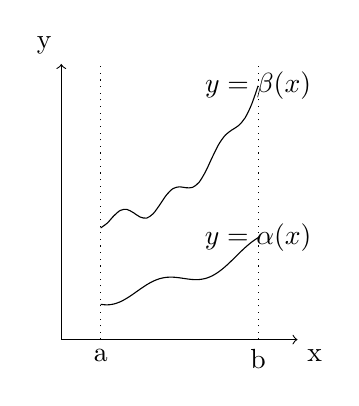
\begin{tikzpicture}
\draw[->] (0,0) -- (3,0) node[anchor=north west] {x};
\draw[->] (0,0) -- (0,3.5) node[anchor=south east] {y};
\draw[dotted] (.5,0) -- (.5,3.5);
\draw[dotted] (2.5,0) -- (2.5,3.5);
\draw (.5,0)  node[anchor=north] {a};
\draw (2.5,0) node[anchor=north] {b};
\draw[domain=.5:2.5,smooth,variable=\x] plot ({\x},{(1/9)*\x*\x*\x+1.5+0.1*sin(10*\x r)}) node {$y=\beta(x)$};
\draw[domain=.5:2.5,smooth,variable=\x] plot ({\x},{(1/9)*\x*\x+0.5+0.1*cos(5*\x r)}) node {$y=\alpha(x)$};
\end{tikzpicture}\\
Se:\\
$a,b\in \R$ con $a<b$\\
$\alpha,\beta\in \cntclass{0}([a,b];R), \forall x\in[a,b] \alpha(x)\le\beta(x)$\\
$A=\{(x,y)\in \R^2: x\in [a,b] $e$ y\in [\alpha(x),\beta(x)] \}$\\
$f\in \cntclass{0}(A;R)$\\
Allora\\
$\iint_Af(x,y)\integrald{x}\integrald{y}=\int_a^b\left(\int_{\alpha(x)}^{\beta{x}}f(x,y)\integrald{y}\right)\integrald{x}$\\
Analogamente.\\
ALTRO GRAFICO....\\
Se:\\
$c,d\in \R$ con $c<d$\\
$\gamma,\delta\in \cntclass{0}([a,b];R), \forall y\in[c,d] \gamma(y)\le\delta(y)$\\
$A=\{(x,y)\in \R^2: x\in [c,d] $e$ x\in [\gamma(y),\delta(y)] \}$\\
$f\in \cntclass{0}(A;R)$\\
Allora\\
$\iint_Af(x,y)\integrald{x}\integrald{y}=\int_c^d\left(\int_{\gamma(y)}^{\delta{y}}f(x,y)\integrald{x}\right)\integrald{y}$
\newpage
\section{Cambiamento di Variabili}
Se:\\
$A\subseteq \R^2$\\
$\varPhi\in \cntclass{1}(A;R^2)$
$\varPhi$ è invertibile
$\varPhi^{-1}\in \cntclass{1}(\varPhi(A);R^2)$\\
$det(D\varPhi)\ne 0$ su $A$\\
$f\in \cntclass{0}(\varPhi(A);R^2)$\\
Allora:\\
\[ \iint_{\varPhi(A)}f(x,y)\integrald{x}\integrald{y}=\iint_A((f\circ g)(u,v))\abs{det(D\varPhi(u,v))}\integrald{u}\integrald{v}\]
La quantità $det(D\varPhi)$ è spesso chiamato DETERMINANTE JACOBIANO (o semplicemente JACOBIANO) della trasformazione $\varPhi$\\
Adesso spieghiamo perché il determinante JACOBIANO, ricordando A1:
\[ \int_g(A)f(x)\integrald{x} = \int_Af(g(t))\integrald{t}\]\\
vari casi\\
...\\
...\\
...\\




\chapter{Successioni e Serie di Funzioni}
\section{Preliminari}
\definition
Sia $f_n:A\subseteq \R\to \R$ una successione ($n\in\N$) , la serie $\sum\limits_{n=09}^{+\infty}f_n$ indica la successione delle somme parziali $S_n = \sum\limits_{i=0}^nf_i$
\observation
Qualunque affermazione fatta in riferimento ad una serie va quindi intesa riferita alla successione delle somme parziali
\begin{description}
	\item[-] La serie è limitata $\bydef$ la successione delle somme parziali è limitata
	\item[-] La serie è illimitata $\bydef$ la successione delle somme parziali è illimitata
	\item[-] La serie è convergente $\bydef$ la successione delle somme parziali è convergente
\end{description}
\observation
Successioni e serie di funzioni possono essere viste:
\begin{enumerate}
	\item come successioni e serie dipendenti da un parametro
	\item come un mezzo per approssimare funzioni
	\item come un primo passo verso lo studio di funzioni (a volte dette operatori o funzionali) che a funzioni associano o numeri o altre funzioni.
\end{enumerate}
\section{Tipi Di Convergenza}
\subsection{Convergenza Puntuale}
\definition
Sia $A\subseteq \R$ e $\left\{f_n:n\in\N\right\}$ una successione di funzioni definite su $A$ a valori in $ \R$. Sia $B\subseteq A$
\begin{description}
	\item[-] la successione $\left\{f_n:n\N\right\}$ è puntualmente convergente su $B$ se $\forall x \in B$, esiste finito il limite $\lim\limits_{n\to\infty}f_n(x)$. In tal caso la funzione $f:B\to  \R$ definito da $f(x)=\lim\limits_{n\to\infty}f_n(x)$
	\item[-] la serie $\sum\limits_{n=0}^{\infty}f_n$ è puntualmente convergente su $B$ se $\forall x \in B$, la serie $\sum\limits_{n=0}^{\infty}f_n(x)$ ammette somma finita. In tal caso la funzione $F:B\to  \R$ definito da $F(x)=\sum\limits_{n=0}^{\infty}f_n(x)$ è la somma della serie la serie $\sum\limits_{n=0}^{\infty}f_n$
\end{description}
\observation
La convergenza puntuale su $A$ della successione $f_n$ verso $f$ è indicata con
$$f_n \pconvarrow f\quad su A$$
\proposition METAPROPOSIZIONE:\\
Sia $f_n:A\to \R$, $B\subseteq A$, $A\subseteq \R$, $f:B\to A$\\
Se $f_n \pconvarrow f$ su $B$ e se $f_n$ ha la proprietà $P$ allora il limite $f$ ha la proprietà $P$.\\

\example $f_n(x)=\frac{1}{n}sin(x)$ con $A\equiv \R$\\
$\lim\limits_{n\to\infty}f_n(x)=\lim\limits_{n\to\infty}\frac{1}{n}sin(x)=0\quad\forall x \in A \Rightarrow f_n \pconvarrow 0$ su $A$.

\example$f_n(x)=e^{nx}$ con $A\equiv \R$
\begin{center}
	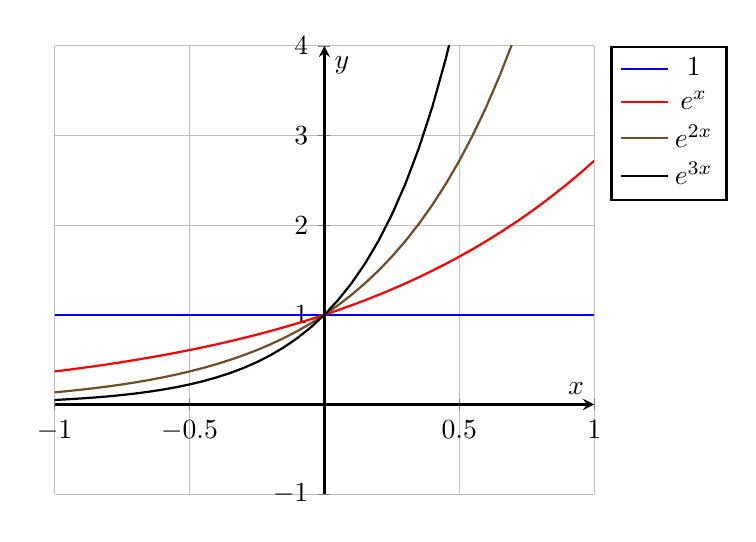
\begin{tikzpicture}[scale=1]
		\begin{axis}[
			xlabel={$x$},ylabel={$y$},
			axis lines=middle,
			samples=41,grid,thick,
			domain=-1:1,
			ymin=-1,ymax=4,
			legend pos=outer north east ]
			\addplot+[no marks] {1}; \addlegendentry{$1$}
			\addplot+[no marks] {e^x}; \addlegendentry{$e^x$}
			\addplot+[no marks]{e^(2*x)}; \addlegendentry{$e^{2x}$}
			\addplot+[no marks]{e^(3*x)}; \addlegendentry{$e^{3x}$}
			\end{axis}
	\end{tikzpicture}
\end{center}
$$\lim\limits_{n\to\infty}e^{nx} = \left\{\begin{matrix} 0 && x<0\\1&&x=0\\\infty&&x>0 \end{matrix}\right.$$
$$f_n \pconvarrow f\quad su B=\left]-\infty,0\right]$$
\observation
La continuità non passa al limite come proprietà $P$

\example $f_n(x)=x^n$ con $A\equiv \R$
\begin{center}
	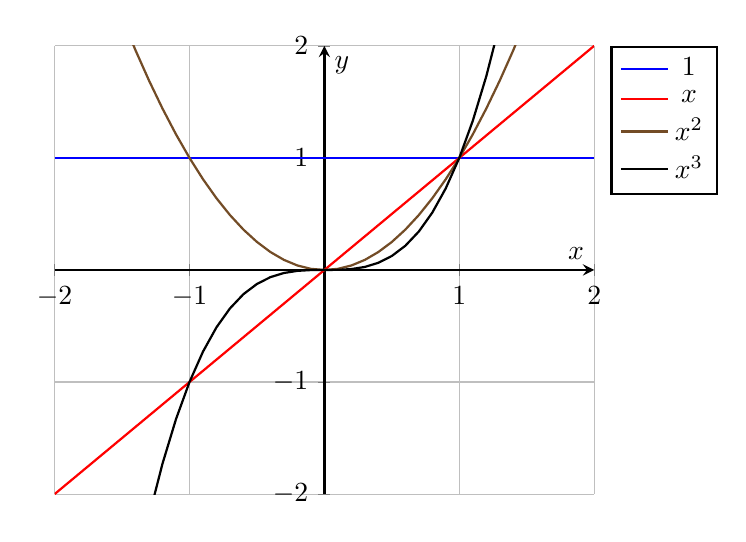
\begin{tikzpicture}[scale=1]
		\begin{axis}[
			xlabel={$x$},ylabel={$y$},
			axis lines=middle,
			samples=41,grid,thick,
			domain=-2:2,
			ymin=-2,ymax=2,
			legend pos=outer north east ]
			\addplot+[no marks] {1}; \addlegendentry{$1$}
			\addplot+[no marks] {x}; \addlegendentry{$x$}
			\addplot+[no marks] {x^2}; \addlegendentry{$x^2$}
			\addplot+[no marks] {x^3}; \addlegendentry{$x^3$}
			\end{axis}
	\end{tikzpicture}
\end{center}
$$\lim\limits_{n\to\infty}x^{n} = \left\{\begin{matrix}+\infty&&x\in\left]1,+\infty\right[\\ 1 && x\in\left\{1\right\}\\0&&x\in\left]-1,1\right[\\\nexists &&x\in\left]-\infty,-1\right] \end{matrix}\right.$$
$$f_n \pconvarrow f\quad su B=\left]-1,1\right]$$
\proposition PROPRIETÀ P:MONOTONIA\\
Sia $f_n:A\to \R$, $B\subseteq A$, $A\subseteq \R$, $f:B\to A$\\
Se $f_n \pconvarrow f$ su $B$ e se $f_n$ è debolmente crescente su $B$ allora il limite $f$ è debolmente crescente su $B$.
\begin{proof}
	Dire che $f_n$ è debolmente crescente su $B$ significa che $$\forall x_1,x_2\in B \quad x_1\le x_2 \Rightarrow fn(x_1)\le f_n(x_2)$$
	se si fa tendere $n\to\infty$ si ha che $f(x_1)\le f(x_2)$, e questo nell'insieme $B$ dove i limiti puntuali delle funzioni esistono per ipotesi
\end{proof}
\observation
Questo vale anche nel caso di funzioni debolmente decrescenti
\observation
se $f_n$ è strettamente crescente/decrescente con le stesse ipotesi non possiamo concludere che il limite puntuale mantenga la stessa proprietà\\
\example $x^n$ con $x\in\left[0,1\right[$ è strettamente crescente ma il limite putuale è costante uguale a zero.
\proposition PROPRIETÀ P:NON NEGATIVA\\
Sia $f_n:A\to \R$, $B\subseteq A$, $A\subseteq \R$, $f:B\to A$\\
Se $f_n \pconvarrow f$ su $B$ e se $f_n$ è non negativa, $f_n\ge 0$, su $B$ allora il limite $f$ è non negativo, $f\ge 0$, su $B$.
\begin{proof}
	Sappiamo che $f(x)=\lim\limits_{n\to\infty}f_n(x)$ $\forall x\in B$.
	Ma $f_n$ è una successione di valori non negativi quindi il limite esiste ed è non negativo.
\end{proof}
\observation
Questo vale anche nel caso di funzioni non positive
\observation
Questa proposizione non può essere estesa al caso di funzioni strettamente positive/negative.\\
\example $	-\frac{e^x}{n}$ con $x\in\left[0,1\right[$ è strettamente negativa ma il limite è costante uguale a zero.
\proposition
Siano $A\subseteq \R, B\subseteq A$, $\left\{f_n:n\in\N\right\}$ una successione di funzioni definite su $A$ con valori in $ \R$. sia $f:B\to \R$ una funzione\\
$f_n \pconvarrow f$ su $B$ per $n\to\infty \iff \forall x\in B,\forall \epsilon >0,\exists\nu\in\N:\forall n>\nu \quad \abs{f_n(x)-f(x)}\le \epsilon$
\begin{proof}
	direttamene dalla definizione...
\end{proof}
\proposition
Siano $A\subseteq \R, B\subseteq A$, $\left\{f_n:n\in\N\right\}$ una successione di funzioni definite su $A$ con valori in $ \R$. Sia $F:B\to \R$ una funzione\\
$\sum\limits_{n=0}^{\infty}f_n \pconvarrow F$ su $B$ per $n\to\infty \iff \forall x\in B,\forall \epsilon >0,\exists\nu\in\N:\forall n>\nu \quad \abs{\sum\limits_{k=0}^{\infty}f_k(x)-F(x)}\le \epsilon$
\begin{proof}
	direttamene dalla definizione...
\end{proof}

\subsection{Convergenza Uniforme}\label{sect:conv_unif}
\begin{definition}[Convergenza Uniforme]
	\label{def:conv_unif}
	Siano $A\subseteq \R$, $B\subseteq A$ e $\left\{f_n:n\in\N\right\}$ una successione di funzioni definite su $A$ a valori in $\R$.
	\begin{itemize}
		\item La \textbf{successione} $\left\{f_n:n\in \N\right\}$ è uniformemente convergente su $B$ se esiste una funzione $f:B\mapsto \R$ tale che:
		$$\lim\limits_{n \to +\infty} \sup\limits_{x\in B}\abs{f_n(x)-f(x)}=0$$\\
		La funzione $f$ è il \textbf{limite uniforme della successione} $f_n$
		\item La \textbf{serie} $\sum\limits_{n=0}^{+\infty}f_n$ è uniformemente convergente su $B$ se esiste una funzione $F:B\mapsto \R$ tale che:
		$$\lim\limits_{n\to +\infty} \sup\limits_{x\in B}\abs{F(x)-\sum\limits_{k=0}^n f_k(x)}=0$$
		la funzione $F$ è il \textbf{limite uniforme della serie} $\sum\limits_{n=0}^{\infty}f_n$
	\end{itemize}
	La convergenza uniforme su $B$ della successione $f_n$ verso $f$ è indicata con "$f_n \uconvarrow f$ su $B$".
\end{definition}
\begin{observation}
	\label{obs:dist_conv_unif}
	la convergenza uniforme equivale alla convergenza rispetto alla distanza $d_{\cntclass{0}}(f,g)=\sup\limits_{x\in A}\abs{g(x)-f(x)}$ ogniqualvolta questa distanza sia definita. La definizione di $d_{\cntclass{0}}(f,g)$ come \textit{distanza} è dimostrata in \hyperref[ex:dim_dist_conv_unif]{\cref*{ex:metriche} (\nameref*{ex:metriche})}\\
	% NOTE The \fullref command was not used on purpose to point this link straight to the right part of the aforementioned exercise
	La $d_{\cntclass{0}}(f,g)$ può anche essere definita attraverso la \textbf{norma} $\norm{k}_{\cntclass{0}}=\sup\limits_{x\in A}\abs{k}$ con $k = f-g$ in quanto, in $\R$ norma e valore assoluto coincidono.
\end{observation}


\proposition
sia $f_n:n\in\N$ con $f:A\subseteq \R\to \R$ e $f:B\subseteq A \to  \R$\\
$f_n \uconvarrow f$ su $B$ per$n\to\infty \iff \forall\epsilon >0, \exists\nu\in\N$  t.c: $\forall n>\nu, \forall x\in B$ vale che $\abs{f_n(x)-f(x)}\le\epsilon$
\proposition
sia $f_n:n\in\N$ con $f:A\subseteq \R\to \R$ e $F:B\subseteq A \to  \R$\\
$\sum\limits_{n=0}^{\infty}f_n \uconvarrow F$ su $B\iff \forall\epsilon >0, \exists\nu\in\N$  t.c: $\forall n>\nu, \forall x\in B$ vale che $\abs{F(x)-\sum\limits_{k=0}^{n}f_k(x)}\le\epsilon$
\observation
La differenza tra queste due proposizioni e le due proposizioni analoghe nel caso di convergenza puntuale giustifica il fatto che la continuità non passa al limite puntuale. Infatti qui $\nu$ dipende solo dalla scelta di $\epsilon$ e le $x$ si guardano tutte insieme, prima invece $\nu$ dipendeva oltre che alla $\epsilon$ anche dalla $x$ questo porta a osservare le $x$ una alla volta.
\proposition Relazione tra convergenza uniforme e puntuale.\\
Sia $f_n:A\subseteq \R\to \R$ e $f:B\subseteq A\to \R$\\
Se $fn \uconvarrow f$ su $B$ allora $fn \pconvarrow f$ su $B$.
\begin{proof}
	se $f_n \uconvarrow f$ su $b$ allora vale che:
	$\forall\epsilon, \exists\nu : \forall n>\nu, \forall x\in B $ vale $\abs{f_n(x)-f(x)}\le\epsilon$ in questo modo si trova un $\nu$ che soddisfa la condizione $\forall x \in B$ quindi $\forall x\in B, \forall\epsilon, \exists\nu : \forall n>\nu $ vale $\abs{f_n(x)-f(x)}\le\epsilon$ quindi $f_n \pconvarrow f$ su B
\end{proof}
\proposition
Sia $f_n:A\subseteq \R\to \R$ e $\overline{f},f:B\subseteq A\to \R$\\
se $f_n \uconvarrow f$ su $B$ e $f_n \uconvarrow \overline{f}$ su $B$ allora $f=\overline{f}$
\begin{proof}
	$f_n \uconvarrow f$ e $f_n \uconvarrow \overline{f}$, quindi è anche vero che $f_n \pconvarrow f$ e $f_n \pconvarrow \overline{f}$ ma il limite puntuale è unico poichè è il limite di una successione. Allora $f=\overline{f}$
\end{proof}
\example $f_n(x)=\frac{1}{n}sin(x)$ con $A\equiv \R$\\
Abbiamo gia calcolato che $f_n \pconvarrow 0$ su $A$.\\
Sia ha anche convergenza uniforme :\\
$$\lim\limits_{n\to\infty}\sup{ \R}\abs{f_n(x)-0} = \lim\limits_{n\to\infty}\sup\limits_{ \R}\abs{\frac{1}{n}sin(x)}$$
Osservo che $\abs{asin(x)}\le\abs{a}$ quindi
$$\lim\limits_{n\to\infty}\sup\limits_{ \R}\abs{\frac{1}{n}sin(x)}\le\lim\limits_{n\to\infty}\frac{1}{n}=0$$
Allora $f_n \uconvarrow f$ su $A$

\example $f_n(x)=sin\left(\frac{1}{n}x\right)$ con $A\equiv \R$
..........\\
..........\\
\proposition
Siano $A\subseteq \R$, $\left\{f_n:A\to \R:n\in\N\right\}$ una successione di funzioni e $f:A\to \R$\\
$f_n \uconvarrow f$ su $A$ e $f_n\in \cntclass{0}(A; \R)\,\,\forall n\in\N$ allora $f\in \cntclass{0}(A; \R)$
\begin{proof}
	DISEGNO\\
	DISEGNO\\
	DISEGNO\\
	DISEGNO\\
	GIURO CHE LA FAROò
	(a distanza di tre anni non son sicurissimo che lo farò)
\end{proof}
\example $f_n(x)=\sqrt{x^2+\frac{1}{n}}$ con $A\equiv \R$\\
%$f_n$ è continua $\forall n$ perchè compositione di funzioni continue.\\
%Il limite puntuale di questa successione di funzioni è $f\left( x \right)=\abs{x}$ su $A$\\
%Si può verificare che $f\left(x\right)=\abs{x}$ è anche limite uniforme su $A$ poichè
%$$ \lim\limits_{n\to\infty}\sup\limits_{x\in A} \abs{\sqrt{x^2+\frac{1}{n}}-\left|x}\right| $$
%analizzando il contenuto del modulo si trova che la sua derivata vale $\frac{1}{2\sqrt{x^2+\frac{1}{n}}}-sgn\left(x\right)$ che si annulla in $x=\pm\sqrt{\frac{1}{4}-\frac{1}{n}}$
..........\\
..........\\
\definition
Siano $A\subseteq \R$, $B\subseteq A$ e $\left\{f_n:A\to \R:n\in\N\right\}$ una successione di funzioni.\\
La successione $\left\{f_n:n\in\N\right\}$ soddisfa alla condizione di Cauchy per la convergenza uniforme su $B \bydef \forall\epsilon>0, \exists\nu\in\N: \forall n,m>\nu, \forall x \in B$ vale $\abs{f_n(n)-f_m(x)}<\epsilon$
\proposition
(Una successione di Cauchy per la convergenza uniforme è uniformemente convergente).\\
Siano $A\subseteq \R$, $B\subseteq A$ e $\left\{ f_n:A\to \R:n\in\N \right\}$ una successione di funzioni.\\
La successione $\left\{ f_n:n\in\N \right\}$ soddisfa alla condizione di Cauchy per la convergenza uniforme su $B$ allora $\exists$ una funzione $f:B\to \R$ t.c.: $f_n \uconvarrow f$ su $B$
\begin{proof}
	La successione $\left\{ f_n:n\in\N\right\}$ soddisfa alla condizione di Cauchy per la convergenza uniforme su $B$ allora $\forall x\in B$ la successione $\left\{ f_n(x) :n\in\N \right\}$ è di Cauchyin $ \R$ allora $\forall x \in B$ la successione $\left\{ f_n(x):n\in\N \right\}$ ha limite in $ \R$.(cioè c'è il limite puntuale).\\
	Sia $f(x)$ questo limite, $f$ è anche il limite uniforme della successione $\left\{ f_n:n\in\N \right\}$, infatti:
	$$\forall\epsilon>0, \exists\nu\in\N: \forall h,k>\nu \forall x\in B \quad \abs{f_h-f_k}<\epsilon$$
	$$\sup\limits_B\abs{f_h(x)-f_k(x)}, \forall h,k>\nu$$
	$$\Rightarrow \abs{f_h(x)-f_k}<\epsilon,\forall h.k>\nu, \forall x \in B$$
	a questo punto si passa al limite e la disuguaglianza diventa debole.
	$$\Rightarrow \lim\limits_{n\to\infty}\abs{f_h(x)-f_k(x)}\le\epsilon, \forall h>\nu, \forall x\in B$$
	$$\Rightarrow\abs{f_h(x)-f(x)}\le\epsilon, \forall h>\nu, \forall x\in B$$
	$$\Rightarrow\sup\limits_B\abs{f_h-f}\le\epsilon, \forall h>\nu$$
	$$\Rightarrow f_n \uconvarrow f\quad su B$$
\end{proof}
\begin{proposition}
	\label{prop:dist_unif_sp_metr_compl}
	Sia $A$ un compatto in $ \R$. In $\cntclass{0}(A; \R)$ sia $d_{\cntclass{0}}=\sup_A\abs{g(x)-f(x)}$. Allora $\left( \cntclass{0}\left(A; \R\right);d_{\cntclass{0}}\right)$ è uno spazio metrico completo.
	\begin{proof}
		prendo $f_n\in \cntclass{0}(A; \R)$ successione di Cauchy in $\cntclass{0}(A; \R)$
		$f_n$ sono di Cauchy rispetto alla convergenza uniforme su $A$
		$\Rightarrow f_n:A\to \R$ e $f_n \uconvarrow f$ su $A$ e $f$ è continua\\ $\Rightarrow\left(f\in \cntclass{0}(A; \R)\right)$\\
		$\Rightarrow\lim\limits_{n\to\infty}f_n=f$ in $\cntclass{0}(A; \R)$\\
		$\Rightarrow\lim\limits_{n\to\infty}d_{\infty}(fn,f)=0\quad\Rightarrow f_n\to f\in \cntclass{0}(A; \R)$
	\end{proof}
\end{proposition}
\begin{corollary} % TODO dimostrare il corollario 19.26 con C di arrivo delle f chiuso
	\label{prop:compl_dist_spm_compl}
\end{corollary}

ESEMPIO:: In dimensione finita non vi è differenza tra "chiuso e limitato" e "compatto", in dimensione infinita cambiamo molte cose.
Prensiamo un insieme chiuso e limitato ma non compatto.\\
In $\cntclass{0}(\left[0,1\right]; \R)$ con $d_\infty(f,g)=\sup_{\left[0,1\right]}\abs{g(x)-f(x)}$, prendiamo l'insieme $C=\overline{B(0,1)}=\left\{f\in \cntclass{0}(\left[0,1\right]; \R):\abs{f(x)}\le 1, \forall x \in\left[0,1\right]\right\}$
\begin{description}
	\item[1] $C$ è limitato: ha diametro finito.
	\item[2] $C$ è chiuso: contiene tutti i sui punti di accumualazione
\end{description}
Se c'è una successione $f_n \uconvarrow f$ su $\left[0,1\right]$ allora voglio mostrare che $f\in C$\\
Se $f_n \uconvarrow f$ su $\left[0,1\right]$ allora $f_n \pconvarrow f$ su $\left[0,1\right]$.
Sappiamo che $\forall n\in\N$ e $\forall x\in \left[0,1\right]$ vale che $-1\le f_n(x)\le 1$.\\
Mandando $n$ al limite si ha che $-1\le f_(x)\le 1$.\\
Inolte $f$ è continua perché limite uniforme di una successione di funzioni continue allora $f\in C$ poiché è una funzione continua compresa tra $-1$ e $1$
\begin{description}
	\item[3] $C$ non è compatto, cioè esiste almeno una successione dalla quale non è possibie estrarre una sottosuccessione convergente nello stesso spazio.
\end{description}
Se ad esempio $f_n(x) = x^n$\\
so che $f_n \pconvarrow f$ su $\left[0,1\right]$ e $f(x)=\left\{\begin{matrix}0&&x\in\left[0,1\right]\\1&&x\in\left\{1\right\}\end{matrix}\right.$\\
Tutta la successione di funzioni $f_n$ converge puntualmente a $f$ quindi se estraggo una sottosuccessione comunque venga scelta questa sottosuccessione converge ancora a $f$ puntualmente. Ma la $f$ non è continua mentre il limite uniforme di funzioni continue è una funzione continua allora nessuna sottosuccessione ammette limite uniforme.\\

ESEMPIO:: OPERATORE DERIVATA 0\\
$$D$$

ESEMPIO:: OPERATORE DERIVATA 1\\
$$D$$

ESEMPIO:: OPERATORE INTEGRALE\\
$$I$$

\proposition
fissati $a,b\in \R$ con $a<b$ se la successione $\left\{f_n:n\in\N\right\}$ in $\cntclass{0}(\left[a,b\right], \R) \uconvarrow f$ su $\left[a,b\right]$\\
$f_n$ e $f$ sono integrabili secondo Rimmmmmmmn allora lasuccessione $\left\{\int_a^bf_n(x)\integrald{x}:n\in\N\right\}$ converge a $\int_a^bf(x)\integrald{x}$
\observation
La convergenza uniforme passa sotto il segno di integrale
$$\int_a^b\left(\lim\limits_{n\to\infty}fn\right)(x)\integrald{x}=\lim\limits_{n\to\infty}\left(\int_a^bfn(x)\integrald{x}\right)$$
\proposition convergono le derivare allora convergono le funzioni\\
Fissati $a,b\in \R$ con $a<b$, si consideri una successione di funzioni $\left\{f_n:n\in\N\right\}$ con $f_n:\left[a,b\right]\to \R$
\begin{enumerate}
	\item $\forall n\in\N, f_n\in \cntclass{1}(\left[a,b\right]; \R)$
	\item $\exists x_0\in\left[a,b\right]: \lim\limits_{n\to\infty}f_n(x_0)=l\in \R$
	\item $\exists g \in \cntclass{0}(\left[a,b\right]; \R):f'_n \uconvarrow g$ su $\left[a,b\right]$
\end{enumerate}
Allora
\begin{enumerate}
	\item $\exists f\in \cntclass{1}(\left[a,b\right]; \R)$
	\item $f_n \uconvarrow f$ su $\left[a,b\right]$
	\item $f'(x)=g(x)$ $\forall x\in\left[a,b\right]$
\end{enumerate}
\begin{proof}
	Per il teorema fondamentale del calcolo integrale
	$$f_n(x)=f_n(x_0)+\int_{x_0}^{x}f_n'(t)\integrald{t}$$
	per $n\to\infty$
	$$f(x)=l+\int_{x_0}^{x}g(t)\integrald{t}$$
	Quindi le $f_n$ convergono puntualmente alla funzione $f(x)$, per la convergenza uniforme calcolo:
	$$ \lim\limits_{n\to+\infty}\sup\limits_{\left[a,b\right]}\abs{f_n(x)-f(x)}\le\lim\limits_{n\to+\infty}(\abs{f_n(x_0)-f(x_0)}+\abs{\int_{x_0}^x \abs{f_n'(t)-g(t)}\integrald{t}})\le$$
	$$\lim\limits_{n\to+\infty}\left[ \abs{f_n(x_0)-f(x_0)}+\abs{b-a}\sup\limits_{\left[a,b\right]}\abs{f_n'(x)-g(x)} \right] = $$
	Questo perché per ipotesi $f'_n=g$ e il limite fa $0$.
	Allora $f_n \uconvarrow f$ su $\left[a,b\right]$\\
	Inoltre si sa che $f_n\in \cntclass{1}$ allora $f_n'\in \cntclass{0}$ allora il limite uniforme di funzioni continue è una funzione continua allora $g$ è una funzione continua.\\
	La $f$ è l'integrale di una funzione continua allora la $f$ è derivabile con derivata continua quindi $f'=g$
\end{proof}
\observation
Necessaria l'ipotesi $f_n(x_0)\to l$.......
\observation
Serve $\left[a,b\right]$ limitato .......\\
.............................\\
................................\\
\begin{corollary}
	\label{coro:deriv_series_series_of_deriv}
	Fissati $a,b\in \R$ con $a<b$, si consideri una successione di funzioni $\left\{f_n:n\in\N\right\}$ con $f_n:\left[a,b\right]\to \R$
	\begin{enumerate}
		\item $\forall n\in\N, f_n\in \cntclass{1}(\left[a,b\right]; \R)$
		\item $\exists x_0\in\left[a,b\right]: \sum\limits_{n=0}^{+\infty}f_n(x_0)=L\in \R$
		\item $\exists g \in \cntclass{0}(\left[a,b\right]; \R): \sum\limits_{n=0}^{+\infty}f'_n \uconvarrow g$ su $\left[a,b\right]$
	\end{enumerate}
	Allora
	\begin{enumerate}
		\item $\exists f\in \cntclass{1}(\left[a,b\right]; \R)$
		\item $\sum\limits_{n=0}^{+\infty}f_n \uconvarrow f$ su $\left[a,b\right]$
		\item $f'(x)=g(x)$ $\forall x\in\left[a,b\right]$
	\end{enumerate}
\end{corollary}
\observation
In altre parole questa proposizione afferma che sotto opportune ipotesi
$$\left(\sum\limits_{n=0}^{+\infty} f_n \right)' =  \sum\limits_{n=0}^{+\infty}f_n'$$
\definition
Siano $A\subseteq  \R$ e $\left\{f_n:n\in\N\right\}$ una successione di funzioni con $f_n:A\to \R$\\
$\sum\limits_{n=0}^{+\infty}f_n$ converge totalmente su $A \bydef \sum\limits_{n=0}^{+\infty}\sup\limits_{A}\abs{f_n(x)}<+\infty$(è convergente)
\observation
la $\sum\limits_{n=0}^{+\infty}\sup\limits_{A}\abs{f_n(x)}$ è una serie numerica
\proposition
Siano $A\subseteq \R$ e $\left\{f_n:n\in\N\right\}$ una successione di funzioni con $f_n:A\to \R$\\
$\sum\limits_{n=0}^{+\infty}f_n$ converge totalmente su $A$ $\Rightarrow$  $\sum\limits_{n=0}^{+\infty}f_n$ converge uniformemente su $A$
\begin{proof}
	$\sum\limits_{n=0}^{+\infty}f_n$ converge totalmente su $A$\\
	$\Rightarrow \sum\limits_{n=0}^{+\infty}\sup\limits_{x\in A}\abs{f_n(x)}<+\infty$\\
	$\Rightarrow \forall\epsilon>0, \exists\nu\in\N: \forall n,m\in\N$ con $m>n>\nu$ vale $\sum\limits_{n=0}^{+\infty}\sup\limits_{x\in A}\abs{f_n}<\epsilon$\\
	$\Rightarrow \forall\epsilon>0, \exists\nu\in\N: \forall n,m\in\N$ con $m>n>\nu$ vale $\sup\limits_{x\in A}\sum\limits_{n=0}^{+\infty}\abs{f_n}<\epsilon$\\
	$\Rightarrow \forall\epsilon>0, \exists\nu\in\N: \forall n,m\in\N$ con $m>n>\nu$ vale $\sup\limits_{x\in A}\abs{\sum\limits_{n=0}^{+\infty}f_n}<\epsilon$\\
	$\Rightarrow \sum\limits_{n=0}^{+\infty}f_n$ soddisfa la condizione di Cauchy per la convergenza uniforme su $A$.
\end{proof}
\observation
Per le serie:\\
Convergenza Totale $\Rightarrow$ Convergenza Uniforme $\Rightarrow$ Convergenza Puntuale.
\subsection{Convergenza Quadratica}
% TODO This subsection is a stub
\begin{proposition}
	\label{def:dist_quadratica}
	% TODO Proposizione 19.49 dal libro

	La definizione di $d_2(f,g)$ come \textit{distanza} è dimostrata in \hyperref[ex:dim_dist_quadratica]{\cref*{ex:metriche} (\nameref*{ex:metriche})}\\
	% NOTE The \fullref command was not used on purpose to point this link straight to the right part of the aforementioned exercise
\end{proposition}
\begin{proposition}
	\label{prop:dist_quad_sp_metr_non_compl}
	% TODO Proposizione 19.52 dal libro
\end{proposition}

\section{Serie di Funzioni Particolari}
Questa sezione è dedicata ad alcune tecniche di approssimazione  basate su serie di funzioni particolari\\
In generale, un'approssimazione si riconduce ad una formula del tipo\\
$$\left[\text{quantità da calcolare}\right]=\left[\text{quantità approssimante}\right]+ errore$$
La qualità dell'approssimazione è descritta dal senso in cui l'errore è piccolo.\\
\subsection{Serie di Potenze}
\definition
Siano $\left\{a_n:n\in\N\right\}$ una successione con $a_n:\N\to\C$ e $z_0\in\C$.\\
Si dice serie di potenze centrata in $z_0 \bydef \sum\limits_{n=0}^{+\infty}a_n\left(z-z_0\right)^n$
\observation
è ovvio che in $z=z_0$ si ha convergenza....???? (dire a zero)
\observation
Per semplicità verrà considerato il caso $z_0=0$
ESEMPIO::$\sum\limits_{n=0}^{+\infty}\frac{x^n}{n!}=1+x+\frac{1}{2} x^2+\ldots+\frac{1}{n!}x^n=e^x$
ESEMPIO::$\sum\limits_{n=0}^{+\infty}x^n=1+x+x^2+\ldots+x^n=\frac{1}{1-x}$
\proposition
Siano $\left\{a_n:n\in\N\right\}$ una successione in $\C$ e $w\in\C$.\\
La serie di potenze $\sum\limits_{n=0}^{+\infty}a_nz^n$ converge in $w$ (cioè $\sum\limits_{n=0}^{+\infty}a_nw^n$ converge) quandi abbiamo la convergenza nella sfera aperta di centro l'origine e raggio $\abs{w}$\\
Allora $\forall r$ con $0<r<\abs{w}$, la serie di potenze $\sum\limits_{n=0}^{+\infty}a_nz^n$ converge totalmente in $B(0,r)$\\
\begin{proof}
	TIKZPICTURE:::::\\
	devo dimostrare che $\sum\limits_{n=0}^{+\infty}\sup\limits_{B(0,r)}\abs{a_nz^n}<+\infty$.\\
	E\' facile vedere che $a_nz^n=a_nw^n\left(\frac{z}{w}\right)^n$.\\
	Quindi passando al modulo e poi al sup si ottiene.\\
	$$\sup\limits_{B(0,r)}\abs{a_nz^n}=\sup\limits_{B(0,r)}\abs{a_nw^n}\abs{\frac{z}{w}}^n\le$$
	Siccome $\sum\limits_{n=0}^{+\infty}a_nw^n$ converge  quindi il suo termine generale tende a $0$.\\
	$$\le\sup\limits_{B(0,r)}\abs{\frac{z}{w}}^n\le\left(\frac{r}{\abs{w}}\right)^n $$
	per ipotesi $r<\abs{w}$ e questo è il termine generale di una serie geometrica convergente.\\
	Ne segue che $\sum\limits_{n=0}^{+\infty}\sup\limits_{B(0,r)}\abs{a_nz^n}$ è maggiorato da $\left( \frac{r}{\abs{w}}\right)^n$ e quindi la serie converge totalmente.
\end{proof}
\observation
Una volta che abbiamo la convergenza totale abbiamo anche quella uniforme.
\proposition la non convergenza in un punto implica la non convergenza fuori dal cerchio\\
Sia ${a_n:n\in\N}$ una successione a valori in $\C$\\
La serie $\sum\limits_{n=0}^{+\infty}a_nz^n$ non  converge in $w$\\
Allora $\forall z\in\C$ con $\abs{z}>\abs{w}$ la serie di potenze $\sum\limits_{n=0}^{+\infty}$ non converge in $z$
\begin{proof}
	\begin{center}
		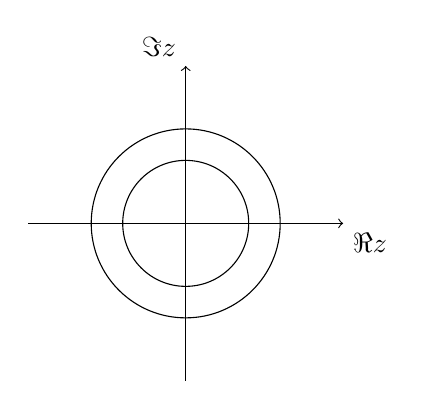
\begin{tikzpicture}[scale=1]
		\draw[->] (-2,0) -- (2,0) node[anchor=north west] {$\Re{z}$};
		\draw[->] (0,-2) -- (0,2) node[anchor=south east] {$\Im{z}$};
		\clip (-2,-2) rectangle (2,2);
		\draw (0,0) circle (1.2cm);
		\draw (0,0) circle (0.8cm);
		\end{tikzpicture}
	\end{center}
	Se per assurdo la serie converge in $z\Rightarrow$ per il teorema precedente  avremmo convergenza in ogni sfera con raggio minore di $\abs{\frac{1}{z}}$. e quindi anche in $w$ questo nega l'ipotesi.ASSURDO.
\end{proof}
\observation
Come è fatto l'insieme su cui si ha convergenza??\\
segue da queste due ultime proposizioni che se $\left\{a_n:n\in\N\right\}$ è una successione in $\C$ allora l'insieme $\left\{z\in\C:\sum\limits_{n=0}^{+\infty}a_nz^n converge\right\}$ è un cerchio.\\Sulla circonferenza non ci soffermaiamo a capire cosa accade poiché tutto può accadere.
\definition
Raggio di convergenza della serie $\sum\limits_{n=0}^{+\infty}a_nz^n\bydef \rho=\sup\left\{r\ge 0 :\sum\limits_{n=0}^{+\infty}a_nz^n converge su B(0,r)\right\}$
\observation
Il raggio di convergenza di una serie di potenze può essere $0$, un numero reale positivo o $+\infty$.
\observation
una definizione come $\rho=\inf\left\{r\ge 0 :\sum\limits_{n=0}^{+\infty}a_nz^n non converge su B(0,r)\right\}$ non sta in piedi poiché questo insieme potrebbe essere vuoto, mentre quello sopra non è mai vuoto, poerché $r=0$ c'è sempre poiché in $0$ si ha sempre convergenza. Ilsecondo potrebbe essere vuoto perché ci sono serie che convergono su tuttoil piano complesso e quindi non si avrebbe nessun $r$ fuori da quale non sia ha convergenza.\\
\proposition CRITERIO DELLA RADICE.\\
Data la serie di potenze $\sum\limits_{n=0}^{+\infty}a_nz^n$, sia $l=\lim\limits_{n\to+\infty}\sqrt[n]{\abs{a_n}}$.\\
Se questo limite esiste, allora il raggio di convergenza è
$\rho =
	\begin{cases}
		0				&	\text{se }l=+\infty\\
		\frac{1}{l} 	&	\text{se }l\in\left]0,+\infty\right[\\
		+\infty 		& 	\text{se }l=0
	\end{cases}
$
\proposition CRITERIO DEL RAPPORTO.\\
Data la serie di potenze $\sum\limits_{n=0}^{+\infty}a_nz^n$, sia $l=\lim\limits_{n\to+\infty}\frac{a_{n+1}}{a_n}$.\\
Se questo limite esiste, allora il raggio di convergenza è
$\rho =
\begin{cases}
0				&	\text{se }l=+\infty\\
\frac{1}{l} 	&	\text{se }l\in\left]0,+\infty\right[\\
+\infty 		& 	\text{se }l=0
\end{cases}
$
ESEMPIO::$e^z=\sum\limits_{n=0}^{+\infty}\frac{1}{n!}z^n$\\
$a_n=\frac{1}{n!} ...  \abs{\frac{a_{n+1}}{a_n}}=\frac{\frac{1}{(n+1)!}}{\frac{1}{n!}}=\frac{n!}{(n+1)!}=\frac{1}{n+1}\overset{n\to+\infty}{\to}0 \Rightarrow \rho=+\infty$\\
ESEMPIO::$sin(z)=\sum\limits_{n=0}^{+\infty}\frac{(-1)^nz^{2n+1}}{(2n+1)!}$ quindi
$a_n =
\begin{cases}
0		&	\text{se }n\text{ è pari}\\
...		&	\text{se }n\text{ è dispari}\\
\end{cases}
$\\
...\\
...\\
...\\
ESEMPIO::$sin(z)=\sum\limits_{n=0}^{+\infty}\frac{(-1)^nz^{2n}}{(2n)!}$ quindi
$a_n =
\begin{cases}
...		&	\text{se }n\text{ è pari}\\
0		&	\text{se }n\text{ è dispari}\\
\end{cases}
$\\
...\\
...\\
...\\
ESEMPIO:: $e^{iy}$ con $y\in \R$
$$e^{iy} = \sum\limits_{n=0}^{+\infty}\frac{1}{n!}(iy)^n = \sum\limits_{n=0}^{+\infty}\frac{1}{(2n)!}(iy)^{2n} + \sum\limits_{n=0}^{+\infty}\frac{1}{(2n+1)!}(iy)^{2n+1} = $$
$$ = \sum\limits_{n=0}^{+\infty}\frac{(-1)^n}{(2n)!}(y)^{2n} + i\sum\limits_{n=0}^{+\infty}\frac{(-1)^n}{(2n+1)!}(y)^{2n+1} = cos(y)+isin(y)$$
\begin{enumerate}
	\item $i^{2n}=\left(i^2\right)^n=(-1)^n$
	\item $i^{2n+1}=i\left(i^2\right)^n=i(-1)^n$
\end{enumerate}
ESEMPIO:: $e^{i\pi}+1=cos(\pi)+i\cdot sin(\pi)=0$\\
ESEMPIO:: $\sum\limits_{n=0}^{+\infty}z^n=\frac{1}{1-z}$ con $\rho=1$
ESEMPIO:: Sia $f(x)=\frac{1}{1+x^2}=\frac{1}{1-(-x^2)} = \sum\limits_{n=0}^{+\infty}(-x^2)^n=\sum\limits_{n=0}^{+\infty}(-1)^nx^{2n}$\\
QUI GRAFICO ..............\\
..........................\\
Questa serieconverge esclusivamente per $\abs{x}<1$, mentre la funzione $f$ è definita su tutto $ \R$, $f\in \cntclass{\infty}( \R; \R)$\\
In $\C$, lafunzione $f(z)=\frac{1}{1+z^2}$ è la somma della serie $\sum\limits_{n=0}^{+\infty}(-1)^nz^{2n}$ che ha raggio di convergenza  $\rho=1$. Infatti, $f(z)$ è singolare sia in $z=i$ sia in $z=-i$.\\
ALTRO GRAFICO::::::::::::::::\\
................................\\

\subsection{Serie di Taylor}
ESEMPIO:: $ln(1+z)$. Calcolare la Serie di Taylor.\\
$$D\left[ln(1+z)\right] = \frac{1}{1+z} = \sum\limits_{n=0}^{+\infty}(-1)^nz^n$$
$$\int \sum\limits_{n=0}^{+\infty}(-1)^nz^n dz = \sum\limits_{n=0}^{+\infty}\frac{(-1)^n}{n+1}z^{n+1}=\sum\limits_{n=1}^{+\infty}\frac{(-1)^{n-1}}{n}z^n$$
\begin{lemma}
	\label{lemma:taylor_rad_convergency}
	Sia $\brackets{a_n:n \in \N}$ una successione a valori in $\C$. Le serie:
	$$\sum_{n=0}^{+\infty} a_n z^n ,\qquad \sum_{n=1}^{+\infty} n a_n z^{n-1} \qquad\text{e}\qquad \sum_{n=0}^{+\infty} \frac{a_n}{n+1}z^{n+1}$$
	hanno lo stesso raggio di convergenza
	\begin{proof}
		Omessa
	\end{proof}
\end{lemma}

\definition
Sia $r\in \R$ con $r>0$. La funzione $f$ si dice analitica su $\left]-r,r\right[ \bydef f(x)=\sum\limits_{n=0}^{+\infty}a_nx^n \quad \forall x\in\left]-r,r\right[$ per opportuni $a_n\in \R$
\observation
In altre parole chiamiamo analitica una funzione che può essere scritta come somma di una serie di potenze convergente su $\left]-r,r\right[$ \\
ESEMPIO:: $x\to e^x$ è analitica su $ \R$\\
ESEMPIO:: $x\to\frac{1}{1+x^2}$ è analitica su $\left]-1,1\right[$\\
\proposition
Se $f$ è analitica su $\left]-r;r\right[$ per $r\in \R$ e $r>0\Rightarrow f\in \cntclass{0}(\left]-r,r\right[; \R)$
\begin{proof}
	$f$ è analitica  allora posso scriverla come $f=\sum\limits_{n=0}^{+\infty}a_nx^n$ cioè la funzione è limite di una serie, se la serie converge totalmente allora converge uniformemente. Il limite uniforme di funzioni continue(in questo caso polinomi) è una funzione continua. cioè la $f$ è continua.
\end{proof}
\proposition PROP+PROOF\\
Sia $f:\left]-r,r\right[\to \R$ e $f$ analitica su $\left]-r,r\right[ \bydef f(x)=\sum\limits_{n=0}^{+\infty}a_nx^n \Rightarrow$ ho convergenza totale $\Rightarrow$ ho convergenza uniforme di funzioni continue
$$\Rightarrow f\in \cntclass{0}(\left]-r,r\right[; \R),\quad a_0=f(0)$$
La serie delle derivate $\sum\limits_{n=0}^{+\infty}na_nx^{n-1}$ converge totalmente su $\left]-r,r\right[$ cioè
$$\sum\limits_{n=0}^{+\infty}f'(x)=\sum\limits_{n=0}^{+\infty}na_nx^{n-1} \uconvarrow g$$
$$\sum\limits_{n=0}^{+\infty}fn(0)\to f(0), f_n\in ????????????$$
Allora la serie delle derivate converge alla derivata della serie
$$\Rightarrow \in \cntclass{1}(\left]-r,r\right[; \R),\quad a_1=f'(0)$$
Questo ragionmento può essere ripetuto:
$$\Rightarrow \forall k\in\N,\quad f\in \cntclass{k}(\left]-r,+r\right[),\quad a_k=k!f^{(k)}(0)$$
e analogamente
$$f\in \cntclass{\infty}(\left]-r,r\right[; \R),\quad f(x)=\sum\limits_{n=0}^{+\infty}\frac{1}{n!}f^{(n)}(0)x^n$$
\observation Qui abbiamo detto se $f$ è analitica $\Rightarrow \ldots$, vorrei fare un qualche tipo di viceversa per poter capire se $f$ è analitica o no.
\proposition
Sia $f:\left]-r,r\right[\to \R$
\begin{center}
	$\left.\begin{matrix}
	f\in \cntclass{\infty}(\left]-r,r\right[; \R)\\
	\sum\limits_{n=0}^{+\infty}\frac{1}{n!}f^{(n)}(0)x^n\text{ converge totalmente su } \left]-r,r\right[\\
	\end{matrix}\right\}\Rightarrow f$ è analitica  .....
\end{center}
Per avere $f$ analitica  necessariamente come ipotesi deve esserci $f\in \cntclass{\infty}$ e $f$ che si può scrivere come sviluppo in serie di Taylor,dalla proposizione precedente. Questo basta? NO\\
ESEMPIO:: $f(x)=\left\{\begin{matrix}0&& x=0\\e^{-\frac{1}{x^2}}&&x\ne 0\end{matrix}\right.$\\
\begin{center}
	\begin{tikzpicture}[scale=1]
	%\draw[->] (0,-4) -- (0,4) node[anchor=north west] {$x$};
	%\draw[->] (-0.1,0) -- (1.2,0) node[anchor=south east] {$y$};
	%\clip (-4,0) rectangle (4,1);
	%\draw[domain=-4:4,smooth,variable=\x] plot ({\x},{{-1/(\x*\x)}});
	\end{tikzpicture}
\end{center}
\begin{enumerate}
	\item $f\in \cntclass{\infty}( \R; \R)$
	\item $\sum\limits_{n=0}^{+\infty}\frac{1}{n!}f^{(n)}(0)x^n$ converge totalmente su $ \R$
	\item $f(x)\ne\sum\limits_{n=0}^{+\infty}\frac{1}{n!}f^{(n)}(0)x^n$
\end{enumerate}
\begin{enumerate}
	\item Vediamo se è $\cntclass{0}$, quindi calcolo $\lim\limits_{x\to 0^{+}}f(x)=\lim\limits_{x\to 0^{-}}f(x)=0=f(0)\Rightarrow f\in \cntclass{0}( \R; \R)$.\\
	Ora calcoliamo la derivata fuori dallo zero, ne facciamo il limite per $x\to 0$ da destra e da sinitra e vediamo cosa succede.\\
	Se $x\ne 0$, $f'(x)=\frac{2}{x^3}e^{-\frac{1}{x^3}}$ e $\lim\limits_{x\to 0^{+}}f'(x)=\lim\limits_{x\to 0^{-}} = 0\Rightarrow f\in \cntclass{1}( \R; \R)$\\
	..........\\
	ancora una derivata.......\\
	..........\\
	Continuando a derivare  avremmo sempre un rapporto di polinomi che moltiplica un esponenziale, e l'esponenziale vince sempre. quindi fa $0$.
	itero il ragionamento......\\
	.......\\
	\item In (1) abbiamo visto  che tutte le derivate nello zero si annullavano, cioè
	$$\forall n\in\N, f^{(n)}(0)=0\Rightarrow \sum\limits_{n=0}^{+\infty}\frac{1}{n!}f^{(n)}(0)x^n$$
	è la serie identicamente nulla  che banalmente converge totalmente su tutto $ \R$
	\item Anche osservandoil grafico è chiaro che la $f$ non è la funzione identicamente nulla cioè è diversa dal suo sviluppo in serie
	$$f(x)\ne\sum\limits_{n=0}^{+\infty}\frac{1}{n!}f^{(n)}(0)x^n$$
\end{enumerate}
Il Problema nasce dall'$o(x^n)$ che scriviamo alla fine dello sviluppo n-esimo di questa funzione, perché l'intorno in cui si ha $o(x^n)$ diventa sempre più piccolo.
GRAFICO...\\
GRAFICO...\\
Mandando l'ordine $n$ all'infinito, l'intervallo su cui si ha l'o piccolo tende a diventare un punto (lo zero). Quindi abbiamo l'ugualianza tra la funzione e il suo sviluppo solo nell'origine.????????NON COMPRESA????\\
????????NON COMPRESA????\\
????????NON COMPRESA????\\
????????NON COMPRESA????\\
Completiamo le ipotesi con la prossima proposizione:
\proposition
Sia $f:\left]-r,r\right[\to \R$
\begin{center}
	$\left.\begin{matrix}
	f\in \cntclass{\infty}(\left]-r,r\right[; \R)\\
	\exists H,K >0 :\forall n\in\N \sup\limits_{\left]-r,r\right[}\abs{f^{(n)}(x)}\le HK^n\\
	\end{matrix}\right\}
	\Rightarrow f(x)=\sum\limits_{n=0}^{+\infty}\frac{1}{n!}f^{(n)}(0)x^n$
\end{center}
\observation
L'ipotesi centrale ............. qui non c'è
\observation
Sia $\sum\limits_{n=0}^{+\infty}(z,w)^n$ una serie di potenze in due variabili.\\
Quando abbiamo due variabili, non si può parlare di raggio di convergenza. Questa serie è una serie geometrica che converge sse $\abs{zw}<1$. è  difficile parlare di raggio di convergenza  perché essendo $z,w\in\C$, se per una variabile servono due dimensioni per due variabili servono quattro dimensioni , e anche se non riusciamo a fare il disegno è evidente che l'insieme su cui la serie converge non è un cerchio(sfera).
\begin{example}[Esempi di Sviluppi in serie di Taylor]
	\label{ex:tay_series_examples}
	\begin{description}
		\item $e^x=\sum\limits_{n=0}^{+\infty}\frac{1}{n!}x^n$
		\item $sin(x)=\sum\limits_{n=0}^{+\infty}\frac{(-1)^n}{(2n+1)!}x^{(2n+1)}$
		\item $sinh(x)=\sum\limits_{n=0}^{+\infty}\frac{1}{(2n+1)!}x^{(2n+1)}$
		\item $cos(x)=\sum\limits_{n=0}^{+\infty}\frac{(-1)^n}{(2n)!}x^{(2n)}$
		\item $cosh(x)=\sum\limits_{n=0}^{+\infty}\frac{1}{(2n)!}x^{(2n)}$
		\item $\frac{1}{1-x}=\sum\limits_{n=0}^{+\infty}x^n$
		\item $ln(1+x)=\sum\limits_{n=1}^{+\infty}\frac{(-1)^{n+1}}{n}x^n$
		\item $arctan(1+x)=\sum\limits_{n=0}^{+\infty}\frac{(-1)^{n}}{2n+1}x^{(2n+1)}$
		\item $\frac{1}{1+x^2}=\sum\limits_{n=0}^{+\infty}(-1)^nx^2n$
		\item $\sum\limits_{n=0}^{+\infty}\frac{1}{n^\lambda}=\left\{\begin{matrix}\text{converge sse } \lambda >1\\ \text{diverge sse } \lambda \le 1 \end{matrix}\right.$
		\item $\sum\limits_{n=0}^{+\infty}q^n=\left\{\begin{matrix}\text{converge sse } \abs{q}<1, S=\frac{1}{1-x}\\ \text{diverge sse } \abs{q}>1\text{ o }q=1\\\nexists \text{ sse } x=-1 \end{matrix}\right.$
	\end{description}
\end{example}
\begin{exercise}
	\label{ex:deriv_func_with_taylor}
	Determinare le derivate delle funzioni
	\begin{itemize}
		\vspace*{-4ex} % I've no idea WTF is wrong with these equations, but the spacing is atrocious without this ugly fix
		\item $x \to \sin x$
		\vspace*{-5ex}
		\item $x \to \cos x$
		\vspace*{-5ex}
		\item $x \to e^x$
		\vspace*{-4ex}
	\end{itemize}
	utilizzando \fullref{ex:tay_series_examples}, il \fullref{lemma:taylor_rad_convergency} ed il \fullref{coro:deriv_series_series_of_deriv}.
\end{exercise}

\subsection{Serie di Fourier}
\definition
Siano $A\subseteq \R$, $f:A\to \R$ e $T>0$, $f$ è $T$-periodica $\bydef \forall x\in A
\left\{\begin{matrix}
x+T\in A\\f(x+T)=f(x)
\end{matrix}\right. $\\


ESEMPIO:: $\lfloor x \rfloor = \text{ parte intera } = \max\left\{k\in\mathbb{Z}:k\le x\right\}$
$$\lfloor \pi \rfloor=3, \quad \lfloor \sqrt{2} \rfloor = 1 \quad \lfloor -e \rfloor = -3 $$
\begin{center}
	\begin{tikzpicture}
		\draw[->] (-4,0) -- (4,0) node[anchor=north west] {$x$};
		\draw[->] (0,-4) -- (0,4) node[anchor=south east] {$y$};

		\foreach \num in {-3,...,3} {
			\draw[line width=0.25mm] (\num , \num) -- (\num+1 , \num);
			\draw[fill=black] (\num , \num) circle (0.1cm);
			\draw (\num+1, \num) circle (0.1cm);
		}
	\end{tikzpicture}
\end{center}
è $1$-periodica.
ESEMPIO:: $mant(x)=\text{ mantissa di x } = x- \lfloor x \rfloor$
\begin{center}
	\begin{tikzpicture}
	\draw[->] (-4,0) -- (4,0) node[anchor=north west] {$x$};
	\draw[->] (0,-4) -- (0,4) node[anchor=south east] {$y$};

	\foreach \num in {-3,...,3} {
		\draw[line width=0.25mm] (\num , 0) -- (\num+1 , 1);
		\draw[fill=black] (\num , 0) circle (0.1cm);
		\draw (\num+1, 1) circle (0.1cm);
	}
	\end{tikzpicture}
\end{center}
è $1$-periodica.
\observation
La funzione costante è $T$-periodica $\forall T>0$, ma non ha un periodo minimo, per questo motivo non la consideriamo.
\observation
Sia $f:A\to \R$ $T$-periodica. Allora possiamo definire $\overline{f}:\overline{A}\to \R$ che sia $2\pi$-periodica data da:
$$x\to f\left(\frac{T}{2\pi}x\right),\quad \overline{A}=\frac{2\pi}{T}A$$
\proposition
Siano $A\subseteq \R$, $f:A\to \R$ e $T>0$\\
$f$ è $T$-periodica $\Rightarrow \forall n\in\N$, $f$ è $nT$-periodica.
\proposition
Sia $f:\left[0,2\pi\right[\to \R \Rightarrow \exists ! \hat{f}: \R\to \R$ t.c.: $\left\{\begin{matrix} \hat{f} 2\pi-periodica\\\hat{f}_{\left|\left[0,2\pi\right]\right.}=f\end{matrix}\right.$
\begin{proof}
	$\forall x\in \R. \exists ! \hat{x}\in\left[0,2\pi\right[$ t.c.: $x=2\pi\cdot k+\hat{x}$ con $k\in\mathbb{Z}$ e $k=\left[??????\right]$\\
	$$\hat{f}(x)=f(\hat{x})$$
\end{proof}
cioè se noi estendiamo una funzione definita su $\left[0,2\pi\right[$ a tutto $ \R$ otteniamo una funzione unica e periodica.
\observation
Con i polinomi di Taylor ........\\
........\\
........\\
........\\
........\\
........\\
\definition
Dati $2n+1$ numeri reali $a_0,a_1,\dotsc,a_n,b_1,\dotsc,b_n$ si dice polinomio trigonometrico di coefficienti $a_0,a_1,\dotsc,a_n,b_1,\dotsc,b_n$ la funzione:
$$\begin{array}{rcl} p: \left[-\pi,\pi\right] & \to &  \R \\ x & \to & \frac{a_0}{2}+\sum\limits_{k=1}^{N}\left(a_ncos(nx)+b_nsin(nx)\right) \end{array}$$
\observation
Essendo un'approssimazione, si deve aggiungere l'errore. Come è fatto?. Per far uscire conti giusti e comodi andrebbe usata la distanza quadratica , ma questo prevede una lunga parte introduttiva, noi allora lo stimiamo con la distanza infinita.
\definition
Date due successioni di numeri reali $\left\{a_n:n\in\N\right\}$,$\left\{b_n:n\in\N\setminus\left\{0\right\}\right\}$, si defininisce serie trigonometrica di coefficienti  $\left\{a_n:n\in\N\right\}$,$\left\{b_n:n\in\N\setminus\left\{0\right\}\right\}$ la serie
$$\begin{array}{rcl} \mathfrak{F}: \left[-\pi,\pi\right] & \to &  \R \\ x & \to & \frac{a_0}{2}+\sum\limits_{k=1}^{+\infty}\left(a_ncos(nx)+b_nsin(nx)\right) \end{array}$$
LEMMA::\\
Se $h,k\in\N$ valgono le seguenti uguaglianze:
\begin{description}
	\item[$\ast$]
	$\int_{-\pi}^{\pi} cos(hx)cos(kx)=
	\left\{\begin{matrix}
	0 &&h\ne k\\\pi&&0\ne h=k\\2\pi&&0=h=k
	\end{matrix}\right.$
	\item[$\ast$] $\int_{-\pi}^{\pi}cos(hx)sin(kx)= 0 $
	\item[$\ast$]
	$\int_{-\pi}^{\pi}sin(hx)sin(kx)=
	\left\{\begin{matrix}
	0 &&h\ne k\text{ oppure }h=k=0\\ \pi&&0\ne h=k
	\end{matrix}\right.$
\end{description}
ESERCIZIO:: IL POLINOMIO DI FOURIER FORNISCE LA MIGLIORE APPROSSIMAZIONE NEL SENSO DELLA DISTANZA QUADRATICA.\\
Sia $f: \realintervalclose{-\pi}{\pi} \mapsto \R$, quale è la funzione a lei più vicina nel senso della distanza quadratica?\\
Fisso $N\in\N$ e prendo il polinomio trigonometrico di grado $N$
$$p_N(x)=\trigonpol{n}{1}{N}$$
con $a_0,a_1,\dotsc,a_n,b_1,\dotsc,b_n\in \R$, il problema è quello di minimizzare $d_2(f,p_n)$ quindi un problema di minimo. Stiamo cercando i coefficienti del polinomio trigonometrico quindi studiamo una funzione $\varphi(a_0,a_1,\dotsc,a_N,b_1,\dotsc,b_N) = \sqrt{\int_{-\pi}^{\pi}\left[f(x)-p_n(x)\right]^2}\integrald{x}$.\\
Essendo la funzione radice quadrata monotona crescente ne studiamo solo il radicando:
$$\varphi(a_0,a_1,\dotsc,a_N,b_1,\dotsc,b_N)=\int_{-\pi}^{\pi}\left[\trigonpol{n}{1}{N}-f(x)\right]^2dx$$
\observation
con $f\in \cntclass{1}$:
$$F(\alpha,\beta,x)=\int_{\alpha}^{\beta}f(x,t)\integrald{t}$$
$$\partial_\alpha F(\alpha,\beta,x)=-f(x,\alpha)\integrald{t}$$
$$\partial_\beta F(\alpha,\beta,x)=f(x,\beta)\integrald{t}$$
$$\nabla_x F(\alpha,\beta,x)=\int_{\alpha}^{\beta}\nabla_xf(x,t)\integrald{t}$$
Qudindi applicando al nostro caso otteniamo
$$\partial_{a_0}\varphi = \int_{-\pi}^{\pi}\partial_{a_0}\left(\left[\trigonpol{n}{1}{N}-f(x)\right]^2\right)\integrald{x}=$$
$$ = \int_{-\pi}^{\pi} \frac{1}{2}2\left(\trigonpol{n}{1}{N}-f(x)\right)\integrald{x}=$$
$$ =  \int_{-\pi}^{\pi} \frac{a_0}{2}\integrald{x} + $$
$$\int_{-\pi}^{\pi} a_1cos(x)\integrald{x} +
\ldots +
\int_{-\pi}^{\pi} a_Ncos(Nx)\integrald{x} + $$
$$\int_{-\pi}^{\pi} b_1sin(x)\integrald{x} +
\ldots +
\int_{-\pi}^{\pi} b_Nsin(Nx)\integrald{x} - $$
$$ \int_{-\pi}^{\pi} f(x)\integrald{x} = $$
L'integrale di una sinusoide su un multiplo intero del periodo è $0$ quindi
$$=\pi a_0-\int_{-\pi}^{\pi}f(x)\integrald{x}$$
Calcolando direttamente anche le derivate seconde si ottiene che
$$\partial^2_{a_0a_0}=\pi\quad\partial^2_{a_0a_n}=0\quad\partial^2_{a_0b_n}=0\quad\forall n=1,\dotsc,N$$

$$\partial_{a_k}\varphi = \int_{-\pi}^{\pi}\partial_{a_k}\left(\left[\trigonpol{n}{1}{N}-f(x)\right]^2\right)\integrald{x}=$$
$$ = \int_{-\pi}^{\pi} 2cos(kx) \left[\trigonpol{n}{1}{N}-f(x)\right]\integrald{x}=$$
$$ =  \cancel{\int_{-\pi}^{\pi} a_0cos(kx)\integrald{x}} + $$
$$\cancel{\int_{-\pi}^{\pi} 2a_1cos(x)cos(kx)\integrald{x}} +
\ldots +
\int_{-\pi}^{\pi} 2a_kcos(kx)cos(kx)\integrald{x}
\ldots +
\cancel{\int_{-\pi}^{\pi} 2a_Ncos(Nx)cos(kx)\integrald{x}} + $$
$$\cancel{\int_{-\pi}^{\pi} 2b_1sin(x)cos(kx)\integrald{x}} +
\ldots +
\cancel{\int_{-\pi}^{\pi} 2b_ksin(kx)cos(kx)}\integrald{x}
\ldots +
\cancel{\int_{-\pi}^{\pi} 2b_Nsin(Nx)cos(kx)\integrald{x}} - $$
$$\int_{-\pi}^{\pi} 2f(x)cos(kx)\integrald{x} = $$
E anche applicando il lemma
$$=2\pi\left[a_k-\int_{-\pi}^{\pi}f(x)cos(kx)\integrald{x}\right]$$
Calcolando direttamente anche le derivate seconde si ottiene che
$$\partial^2_{a_ka_0}=\pi\quad\partial^2_{a_ka_n}=
\left\{\begin{matrix}
0&&n\ne k\\2\pi&&n=k
\end{matrix}\right.
\quad\partial^2_{a_kb_n}=0\quad\forall n=1,\dotsc,N$$

$$\partial_{b_k}\varphi = \int_{-\pi}^{\pi}\partial_{b_k}\left(\left[\trigonpol{n}{1}{N}-f(x)\right]^2\right)\integrald{x}=$$
$$ = \int_{-\pi}^{\pi} 2sin(kx) \left[\trigonpol{n}{1}{N}-f(x)\right]\integrald{x}=$$
$$ =  \cancel{\int_{-\pi}^{\pi} a_0sin(kx)\integrald{x}} + $$
$$\cancel{\int_{-\pi}^{\pi} 2a_1cos(x)sin(kx)\integrald{x}} +
\ldots +
\cancel{\int_{-\pi}^{\pi} 2a_kcos(kx)sin(kx)}\integrald{x}
\ldots +
\cancel{\int_{-\pi}^{\pi} 2a_Ncos(Nx)sin(kx)\integrald{x}} + $$
$$\cancel{\int_{-\pi}^{\pi} 2b_1sin(x)sin(kx)\integrald{x}} +
\ldots +
\int_{-\pi}^{\pi} 2b_ksin(kx)sin(kx)\integrald{x}
\ldots +
\cancel{\int_{-\pi}^{\pi} 2b_Nsin(Nx)sin(kx)\integrald{x}} - $$
$$\int_{-\pi}^{\pi} 2f(x)sin(kx)\integrald{x} = $$
E anche applicando il lemma
$$=2\pi\left[b_k-\int_{-\pi}^{\pi}f(x)cos(kx)\integrald{x}\right]$$
Calcolando direttamente anche le derivate seconde si ottiene che
$$\partial^2_{b_ka_0}=\pi\quad\partial^2_{b_ka_n}=
\left\{\begin{matrix}
0&&n\ne k\\2\pi&&n=k
\end{matrix}\right.
\quad\partial^2_{b_kb_n}=0\quad\forall n=1,\dotsc,N$$
Si verifica la condizione $\nabla\varphi = 0$ con
\begin{description}
	\item[$\ast$] $a_0=\frac{1}{\pi}\int_{-\pi}^{\pi}f(x)\integrald{x}$
	\item[$\ast$] $a_k=\frac{1}{\pi}\int_{-\pi}^{\pi}f(x)cos(kx)\integrald{x}$
	\item[$\ast$] $b_k=\frac{1}{\pi}\int_{-\pi}^{\pi}f(x)sin(kx)\integrald{x}$
\end{description}
La matrice Hessiana di $\varphi$ risulta $$H_{\varphi}=\left[\begin{matrix}
\pi&&0&&0&&\ldots&&0\\
0&&2\pi&&0&&\ldots&&0\\
0&&0&&2\pi&&\ldots&&0\\
\vdots&&\vdots&&\vdots&&\ddots&&\vdots\\
0&&0&&0&&0\ldots&&2\pi
\end{matrix}\right]$$
è una matrice diagonale quindi si leggono direttamente tutti gli autovalori che sono strettamente positivi quindi la forma quadratica è definita positiva ed il punto in questione è un punto di minimo assoluto.
\definition
Sia $f: \realintervalclose{-\pi}{\pi} \mapsto \R$, i coefficienti di Fourier di $f$ sono (ovviamente $f$ deve essere tale da ammetterli finiti):
$$a_0=\frac{1}{\pi}\int_{-\pi}^{\pi}f(x)\integrald{x}$$
$$a_k=\frac{1}{\pi}\int_{-\pi}^{\pi}f(x)cos(kx)\integrald{x}\quad k\in\N\setminus{\left\{0\right\}}$$
$$b_k=\frac{1}{\pi}\int_{-\pi}^{\pi}f(x)sin(kx)\integrald{x}\quad k\in\N\setminus{\left\{0\right\}}$$
La serie di Fourier di $f$ è
$$\trigonpol{k}{1}{+\infty}$$
\proposition
Sia $F: \realintervalclose{-\pi}{\pi} \mapsto \R$ la somma della serie trigono metrica definita dai coefficienti $\left\{a_n:n\in\N\right\}$ e $\left\{a_n:n\in\N\setminus{\left\{0\right\}}\right\}$ e la serie trigonometrica converge uniformemente allora $F$ è una funzione continua e
$$a_k=\frac{1}{\pi}\int_{-\pi}^{\pi}F(x)cos(kx)\integrald{x}\quad k\in\N$$
$$b_k=\frac{1}{\pi}\int_{-\pi}^{\pi}F(x)sin(kx)\integrald{x}\quad k\in\N\setminus{\left\{0\right\}}$$
ESEMPIO+DIMOSTRAZIONE:::\\
sia $f(x)=\trigonpol{n}{1}{+\infty}$. Allora:\\
$$a_0=\frac{1}{\pi}\int_{-\pi}^{\pi}f(x)\integrald{x}=\frac{1}{\pi}\int_{-\pi}^{\pi}\trigonpol{n}{1}{+\infty}\integrald{x}=$$
$$
= \frac{1}{\pi}\int_{-\pi}^{\pi}\frac{a_0}{2} +
\frac{1}{\pi}\int_{-\pi}^{\pi}\left(\sum\limits_{n=1}^{+\infty} a_ncos(nx)\right)\integrald{x} +
\frac{1}{\pi}\int_{-\pi}^{\pi}\left(\sum\limits_{n=1}^{+\infty} b_ncos(nx)\right)\integrald{x}
$$
Poiché si ha convergenza uniforme si può portare l'integrale dentro la sommatoria.
$$
= \frac{1}{\pi}\int_{-\pi}^{\pi}\frac{a_0}{2} +
\cancel{\frac{1}{\pi}\sum\limits_{n=1}^{+\infty}\int_{-\pi}^{\pi} a_ncos(nx)\integrald{x}} +
\cancel{\frac{1}{\pi}\sum\limits_{n=1}^{+\infty}\int_{-\pi}^{\pi} b_ncos(nx)\integrald{x}}=
$$
$$=\frac{1}{\pi}\frac{a_0}{2}\left(\pi-(-\pi)\right)=a_0$$


$$a_k=\frac{1}{\pi}\int_{-\pi}^{\pi}f(x)cos(kx)\integrald{x}=$$
$$\frac{1}{\pi}\left[
\cancel{\int_{-\pi}^{\pi}\frac{a_0}{2}cos(kx)\integrald{x}}+
\int_{-\pi}^{\pi}\left(\sum\limits_{n=1}^{+\infty}a_ncos(nx)cos(kx)\right)\integrald{x}+
\cancel{\int_{-\pi}^{\pi}\left(\sum\limits_{n=1}^{+\infty}b_nsin(nx)cos(kx)\right)\integrald{x}}
\right]=$$
$$\frac{1}{\pi}\left[
\cancel{\int_{-\pi}^{\pi}\left(\sum\limits_{n=1}^{k-1} a_ncos(nx)cos(kx)\right)\integrald{x}}+
\int_{-\pi}^{\pi}a_kcos(kx)cos(kx)\integrald{x}+
\cancel{\int_{-\pi}^{\pi}\left(\sum\limits_{n=k+1}^{+\infty}a_ncos(nx)cos(kx)\right)}\integrald{x}
\right]=$$
$$=\frac{1}{\pi}\pi a_k=a_k$$

$$b_k=\frac{1}{\pi}\int_{-\pi}^{\pi}f(x)sin(kx)\integrald{x}=$$
$$\frac{1}{\pi}\left[
\cancel{\int_{-\pi}^{\pi}\frac{a_0}{2}sin(kx)\integrald{x}}+
\int_{-\pi}^{\pi}\left(\sum\limits_{n=1}^{+\infty}a_ncos(nx)sin(kx)\right)\integrald{x}+
\cancel{\int_{-\pi}^{\pi}\left(\sum\limits_{n=1}^{+\infty}b_nsin(nx)sin(kx)\right)\integrald{x}}
\right]=$$
$$\frac{1}{\pi}\left[
\cancel{\int_{-\pi}^{\pi}\left(\sum\limits_{n=1}^{k-1} a_ncos(nx)sin(kx)\right)\integrald{x}}+
\int_{-\pi}^{\pi}a_kcos(kx)sin(kx)\integrald{x}+
\cancel{\int_{-\pi}^{\pi}\left(\sum\limits_{n=k+1}^{+\infty}a_ncos(nx)sin(kx)\right)}\integrald{x}
\right]=$$
$$=\frac{1}{\pi}\pi b_k=b_k$$
\observation
Se $d_2(f,\text{polinomio di Fourier})$ \`{e} minima $\Rightarrow$ il polinomio di Fourier \`{e} costruito con i coefficienti di Fourier di $f$.
\observation
Se $f$ \`{e} somma di una serie di funzioni $\Rightarrow$ i coefficienti della serie sono i coefficienti di Fourier.
\observation
Funzioni diverse possono avere gli stessi coefficienti di Fourier, cio\`{e} $\exists f,g$ con $f\ne g$ ma $f$ e $g$  hanno gli stessi coefficienti di Fourier.
ESEMPIO::
\begin{center}
	\begin{tikzpicture}
		\draw[->] (-2,0) -- (2,0) node [anchor=north west]{$x$};
		\draw[->] (0,0) -- (0,2);
		\clip (-2,0) rectangle (2,2);
		\draw[domain=-2:2,smooth,red,variable=\x] plot ({\x},{1}) node{$f$};
		\draw[domain=-2:2,smooth,blue,variable=\x] plot ({\x},{1}) node{$g$};
	\end{tikzpicture}
	SISTEMARE,
\end{center}
\observation
I coefficienti di Fourier non possono identificare univocamente puntualmente una funzione.
\subsubsection{Punto Di Vista Geometrico}
In $R^2$ Ci sono $2$ vettori $\hat{i},\hat{j}$ della base, se $\underline{v}\in \R^2 \Rightarrow \underline{v}=v_1\cdot \hat{i}+v_2\cdot \hat{j}$ con $v_1,v_2$ componenti di $\underline{v}$\\
Calcolo delle componenti:\\
$$\underline{v}\cdot \hat{i} = v_1\cdot \hat{i\cdot }\hat{i}+v_2\cdot \hat{j}\cdot \hat{i}=v_1$$
$$\underline{v}\cdot \hat{j} = v_1\cdot \hat{i}\cdot \hat{j}+v_2\cdot \hat{j}\cdot \hat{j}=v_2$$
Questo vale perché $\hat{i},\hat{j}$ è una base ortonormale.
In $R^3$ Ci sono $3$ vettori $\hat{i},\hat{j},\hat{k}$ della base, se $\underline{v}\in \R^3 \Rightarrow \underline{v}=v_1\hat{i}+v_2\hat{j}+v_3\hat{k}$ con $v_1,v_2,v_3$ componenti di $\underline{v}$\\
Calcolo delle componenti:
$$ v_1=\underline{v}\cdot \hat{i}\quad v_2=\underline{v}\cdot \hat{j}\quad v_3=\underline{v}\cdot \hat{k}  $$
In $R^n$ Ci sono $n$ vettori $e_1,e_2,\dotsc,e_n$ della base, se $\underline{v}\in \R^n \Rightarrow \underline{v}=v_1\cdot e_1+v_2\cdot e_2+\ldots+v_n\cdot e_n=\sum\limits_{k=1}^{n}v_k\cdot e_k$ con $v_1,v_2,\dotsc,v_n$ componenti di $\underline{v}$\\
Calcolo delle componenti:
$$v_k=\underline{v}\cdot e_k$$
\\
Con le Serie di Fourier su esegue la stessa operazione sullo spazi $\cntclass{0}(\realintervalclose{-\pi}{\pi}; \R)$. Come elementi di base si ha un insieme di funzioni:
\begin{enumerate}
	\item $c_0:x\to 1$
	\item $c_1:x\to cos(x)$
	\item $c_2:x\to cos(2x)$
	\item $\ldots$
	\item $c_n:x\to cos(nx)$
	\item $s_1:x\to sin(x)$
	\item $s_2:x\to sin(2x)$
	\item $\ldots$
	\item $s_n:x\to sin(nx)$
\end{enumerate}
Si possono osservare due cose:
\begin{enumerate}
	\item Sono tutte funzioni linearmente indipendenti, poiché l'unica combinazione lineare di questi elementi che da l'elemento nullo è quella a coefficenti tutti nulli.
\end{enumerate}
\definition
Il prodotto scalare in $\cntclass{0} \bydef \left<f,g\right>=\int_{-\pi}^{\pi}f(x)g(x)\integrald{x}$
Altre simbologie usate sono: $ f\bullet g $, $(f|g)$
\observation linearità\\
$$\left<(\alpha\cdot f+\beta\cdot g), h \right>= \int_{-\pi}^{pi} (\alpha\cdot f(x)+\beta\cdot g(x))\cdot h(x) \integrald{x}=$$
$$=\int_{-\pi}^{pi} \left[\alpha\cdot f(x)\cdot h(x)+\beta\cdot g(x)\cdot h(x) \right]\integrald{x}= $$
$$=\alpha\int_{-\pi}^{pi} \cdot f(x)\cdot h(x) \integrald{x}+\beta\int_{-\pi}^{pi} \cdot g(x)\cdot h(x) \integrald{x} =$$
$$\alpha\left<f,h\right>+\beta\left<g,h\right>$$

Ripetiamolo stesso ragionamento applicato in $ \R^2, \R^3,$ e $ \R^n$ per ricavare le componenti, possiamo fare questo perché abbiamo una base e abbiamo definito un prodotto scalare.\\
Se $f(x)=\trigonpol{n}{1}{+\infty} \Rightarrow $
$$a_0=\frac{1}{\pi}\int_{-\pi}^{\pi}f(x)dxs=\frac{1}{\pi}\left<f,c_0\right> $$
$$a_k=\frac{1}{\pi}\int_{-\pi}^{\pi}f(x)cos(kx)\integrald{x}=\frac{1}{\pi}\left<f,c_k\right> $$
$$b_k\frac{1}{\pi}\int_{-\pi}^{\pi}f(x)sin(kx)\integrald{x}=\frac{1}{\pi}\left<f,s_k\right>$$
Quindi come prima le componenti di un vettore si ottengono moltiplicando(prodotto scalare) il vettore per gli elementi della base.\\
PER IL LEMMA:\\
$$
\left<c_h,c_k\right>=
\left\{\begin{matrix}
0&&h\ne k\\
2\pi&&0=h=k\\
\pi&&0\ne h=k\\
\end{matrix}\right.
$$
$$ \left<c_h,s_k\right>=0$$
$$
\left<s_h,s_k\right>=
\left\{\begin{matrix}
0&&h\ne k\\
\pi&&0\ne h=k\\
\end{matrix}\right.
$$
Il prodotto scalare di elementi diversi è nullo quindi la base è ortogonale, ma non è ortonormale in quanto il prodotto scalare tra due elementi diversi della base non è unitario.(ecco perché gli $\frac{1}{\pi})$ e $\frac{a_0}{2}$)\\
In generale in geometria non è difficile normalizzare una base, è sufficiente dividere tutti gli elementi per la loro norma. In questo caso decidiamo di non applicare questo ragionamento poiché la norma vale $\sqrt{\pi}$ e se normalizziamo dobbiamo aggiungere questo termini ......\\
Il prodotto scalare in $\cntclass{0}$ è molto legato alla $d_2$ infatti:
$$\norm{f}_2=\sqrt{\left<f,f\right>}=\sqrt{\int_{-\pi}^{\pi}f(x)\cdot f(x)\integrald{x}}\sqrt{\int_{-\pi}^{\pi}\left[f(x)\right]^2dx}$$
Continuano le analogie:\\
In $ \R^2$ ........\\
In $ \R^3$ .........\\
.....\\
......\\
......\\
.....\\
Passando in dimensione infinita, abbiamo una funzione $f$ (come vettore $\underline{v}$) nello spazio, e fare il polinomio di Fourier  vuole dire proiettare la funzione $f$ in uno spazio fatto dai primi $2n+1$ elementi della base che è uno spazio di dimensione finita.\\
\\
Esempio:::: Non ogni funzione ammette coefficienti di Fourier finiti. La funzione
$$\begin{array}{rcl} f: \left[-\pi,\pi\right] & \to &  \R \\
x & \to & \left\{\begin{matrix} 0 && x=0\\\frac{1}{x^2}&&x\ne 0 \end{matrix}\right. \end{array}$$
non ammette coefficienti di Fourier finiti.\\
Esempio::: Una funzione può ammettere tutti i coefficienti di Fourier finiti ed una serie di Fourier convergente, ma ad un limite diverso da $f$.La funzione.
$$\begin{array}{rcl} f: \left[-\pi,\pi\right] & \to &  \R \\
x & \to & \left\{\begin{matrix} -1 && x<0\\1&&x>0 \end{matrix}\right. \end{array}$$
ha coefficienti di Fourier
$$a_k=0\quad\forall k,\quad\quad \left\{\begin{matrix}0 && k\text{ dispari }\\ \frac{4}{k\pi}&& k \text{ pari } \end{matrix}\right.$$
e serie di Fourier
$$ F_f(x)= \frac{4}{\pi}\sum\limits_{k=0}^{+\infty}\frac{sin(2h+1)x}{2h+1} $$
questa serie converge puntualmente in $0$ ma $F_f(0)\ne f(0)$\\

ESEMPIO:: Due funzioni diverse possono avere gli stessi coefficienti di Fourier:
$$\begin{array}{rcl} f: \left[-\pi,\pi\right] & \to &  \R \\
x & \to & \left\{\begin{matrix} -1 && x<0\\0&&x= 0\\1&&x>0 \end{matrix}\right.\end{array}$$
$$\begin{array}{rcl} g: \left[-\pi,\pi\right] & \to &  \R \\
x & \to & \left\{\begin{matrix} -1 && x<0\\\pi&&x= 0\\1&&x>0 \end{matrix}\right.\end{array}$$
\observation
Sia $f$ una funzione pari $\Rightarrow bn=0 \forall n=1,2,\dotsc,+\infty$
\observation
Sia $f$ una funzione dispari $\Rightarrow an=0 \forall n=0,1,,\dotsc,+\infty$
\observation
Siano
$$f(x)=\frac{a_0}{2}+\sum\limits_{n=}^{+\infty}\left(a_ncos(nx)+b_nsin(nx)\right)$$
$$\varphi(x)=\frac{\alpha_0}{2}+\sum\limits_{n=}^{+\infty}\left(\alpha_ncos(nx)+\beta_nsin(nx)\right)$$
Allora
$$ F(x)=(f+\varphi)(x)=\frac{A_0}{2}+\sum\limits_{n=}^{+\infty}\left(A_ncos(nx)+B_nsin(nx)\right)$$
con $A_n=a_n+\alpha_n$. $B_n=b_n+\beta_n$.
cioè i coefficienti di Fourier dipendono linearmente dalla funzione.\\
Esempio::: $B_3=\frac{1}{\pi}\int_{-\pi}^{\pi}F(x)sin(3x)\integrald{x}=\frac{1}{\pi}\int_{-\pi}^{\pi}(f(x)+\varphi(x))sin(3x)\integrald{x}=$\\
$\frac{1}{\pi}\left[\int_{-\pi}^{\pi}f(x)sin(3x)\integrald{x}+\int_{-\pi}^{\pi}\varphi(x)sin(3x)\integrald{x}\right]=b_3+\beta_3$\\
Sia $f(x)=\frac{a_0}{2}+\sum\liminf_{n=1}^{+\infty}\left(a_ncos(nx)+b_ncos(nx)\right)$ allora $F=4f=\frac{A_0}{2}+\sum\limits_{n=1}^{+\infty}\left(A_ncos(nx)+B_ncos(nx)\right)$ con $A_n=4a_n$, $B_n=4b_n$\\
ESEMPIO
Esempio:::$B_3=\frac{1}{\pi}\int_{-\pi}^{\pi}F(x)sin(3x)\integrald{x}=\frac{1}{\pi}\int_{-\pi}^{\pi}4f(x)sin(3x)\integrald{x}=4b_3$\\
\begin{definition}[Funzione Continua a Tratti]
	Siano $a,b\in \R$ con $a<b$, una funzione $f:\realintervalclose{a}{b} \mapsto \R$. Allora $f$ è \textbf{continua a tratti} se esiste un numero finito di punti $x_1,x_2,\dotsc,x_n$ tali che:
	\begin{enumerate}
		\item In ogni punto di $\realintervalclose{a}{b}\setminus\left\{x_1,x_2,\dotsc,x_n\right\}$ f è continua
		\item $i=1,2,\dotsc,n$ esistono finiti entrambi i limiti:
		$$\lim\limits_{x\to x_i^{-}}f(x)\quad \lim\limits_{x\to x_i^{+}}f(x)$$
	\end{enumerate}
\end{definition}

\observation
Dato $A\subseteq \R$ e data una funzione $f:A \mapsto \R$, se $x_0$ è punto interno ad $A$, è comoda la notazione
$$f(x-)=\lim\limits_{\xi\to x^{-}}f(\xi)\quad f(x+)=\lim\limits_{\xi\to x^{+}}f(\xi)$$
Ovviamente se $f$ è continua in $x$ allora $f(x-)=f(x)=f(x+)$
ESEMPIII:::\\
GRAFICO::::\\
GRAFICO::::\\
.......\\
.......\\
.......\\
.......\\
\proposition
Sia $f: \realintervalclose{-\pi}{\pi} \mapsto \R$, $f$ è continua a tratti $\Rightarrow$ esistono finiti tutti i coefficienti di Fourier di $f$
\proposition
Sia $f: \realintervalclose{-\pi}{\pi} \mapsto \R$,\\
-$f$ è continua a tratti\\
-$\forall \overline{x} \in\realintervalclose{-\pi}{\pi}$, esistono finiti:\\
$$ \lim\limits_{x\to\overline{x}^{-}}=\frac{f(x)-f(\overline{x}-)}{x-\overline{x}} $$
$$ \lim\limits_{x\to\overline{x}^{+}}=\frac{f(x)-f(\overline{x}+)}{x-\overline{x}} $$
Allora:\\
La serie di Fourier di $f$ converge puntualmente in $\overline{x}$ e $F_f(\overline{x})=\frac{f(\overline{x}-)-\overline{x}+}{2}$ (che è il punto medio del salto.)
\observation NIENTE CUSPIDI E NIENTE TANGENZE VERTICALI.

\corollary
Sia $f: \realintervalclose{-\pi}{\pi} \mapsto \R$,\\
$f$ è continua a tratti.\\
Sia $\overline{x}\in\realintervalclose{-\pi}{\pi}$ un punto in cui $f$ è derivabile. Allora la serie di Fourier $F_f$ di $f$ converge in $\overline{x}$ e $F_f(\overline{x})=f(\overline{x})$
\proposition
Sia $f: \realintervalclose{-\pi}{\pi} \mapsto \R$.Se:\\
\begin{description}
	\item[$\ast$] $f\in \cntclass{0}(\realintervalclose{-\pi}{\pi}; \R)$
	\item[$\ast$] $\exists x_1,x_2,\dotsc,x_n\in\realintervalclose{-\pi}{\pi}$ t.c.:
	\begin{description}
		\item[-] $f$ è derivabile in $x$
		\item[-] $f'$ continua in $x$
	\end{description}
	\item[$\ast$] $\forall i=1,2,\dotsc,n$ e $\forall x\in\realintervalclose{-\pi}{\pi}$ esistono finiti
	$$\lim\limits_{x\to x_i^{-}}\frac{f(x)-f(x_i-)}{x-x_i}\qquad \lim\limits_{x\to x_i^{+}}\frac{f(x)-f(x_i+)}{x-x_i}$$

\end{description}
Allora\\
La serie di Fourier $F_f$ di $f$ converge a $f$ uniformemente su $\realintervalclose{-\pi}{\pi}$
\corollary
Sia $f: \realintervalclose{-\pi}{\pi} \mapsto \R$, e $f\in \cntclass{1}(\realintervalclose{-\pi}{\pi}; \R)$.\\
Allora la serie di Fourier di $F_f$ di $f$ converge uniformemente a $f$ su $\realintervalclose{-\pi}{\pi}$.
\chapter{Equazioni Differenziali}
\section{Preliminari}
Equazione è un uguaglianza in cui c'è almeno una incognita.\\
Equazione differenziale è un particolare tipo di equazione e stabilisce una relazione tra la funzione incognita e le sue derivate.In un equazione funzionale si cerca l'uguaglianza di: insieme di arrivo, insieme di partenza, corrispondenza.\\
Non è necessario sapere il valore della soluzione ma sapere che ne esiste una.????????\\\\
Equazione differenziale ordinaria:\\
1- La funzione incognita è funzione di una sola variabile, solitamente il tempo.\\
2- La funzione incognita e le sue derivate sono calcolate allo stesso istante di tempo.\\
\begin{definition}[Equazione differenziale]
	\label{def:equaz_diff}
	Si dice equazione differenziale ordinaria di ordine $n$ nella funzione incognita $x\in \R^k$ un espressione del tipo:
	$$f(t,x, x',\ldots,x^{(n)})=0$$
	dove $f:A\to \R^m$, $A\subseteq \R^{1+(1+n)k}$ e $t\in \R$.\\
	$m$ e $k$ caratterizzano il problema e son dunque libere. La dimensione di partenza $1+(1+n)k$ del problema è obbligata e dovuta alla somma di:
	\begin{itemize}
		\item $1 = dim(t)$
		\item $(1+n)k$
		\begin{itemize}
			\item $(1+n)$ il numero totale delle funzioni: $n$ derivate ed $x$ stessa
			\item $k$ la dimensione dell'insieme di partenza di ogni funzione incognita
		\end{itemize}
	\end{itemize}
	\textbf{Soluzione} di questa equazione differenziale è una qualunque funzione $x:I\to \R^k$ definita su un intervallo $I\subseteq \R$, derivabile $n$ volte in $I$ (e dunque continua in $I$) e tale che $\forall t\in I$
	$$t,x, x',\ldots,x^{(n)}) \in A$$
	$$f(t,x, x',\ldots,x^{(n)})=0$$
	\textbf{Soluzione massimale} di un equazione differenziale ordinaria è una soluzione $x_m:I_m\to \R^k$ tale che nessuna soluzione possa essere definita in un intervallo $I$ con $I_m\subseteq I$
\end{definition}
\begin{note} \hypertarget{def:equaz_diff_sol}{}
	Dalla definizione segue che $x \in \circdot{A}$, in quanto se non fosse in $\circdot{A}$ sarebbe di frontiera, ma un punto di frontiera non può essere derivabile.
\end{note}
\begin{note}
	Un'equazione differenziale ammette, in generale, infinite soluzioni.
\end{note}
\begin{note} \hypertarget{note:diff_eq_sol_definit_set}{}
	La soluzione di un'equazione differenziale può, analiticamente, essere definita su un intervallo $J\supset I$ ($I$ intervallo di definizione della funz. differenziale $f$). Non ha però senso considerare il suo comportamento al di fuori di $I$, in quanto non ha valore dal punto di vista del sistema. Per questo motivo $J$ sarà sempre considerato $J\subseteq I$
\end{note}
\begin{note}
	dalla \fullref{def:equaz_diff} segue che l'insieme di definizione della soluzione di un'equazione differenziale può essere solo un intervallo
\end{note}
\begin{example}
	Presa l'equazione differenziale $ x'=1$, essa è risolta da $x(t) = t + \alpha$ per ogni $\alpha\in\R$
\end{example}
\begin{exercise}
	La soluzione di un'equazione differenziale ordinaria non può avere 3 asintoti.
	\begin{solution}
		La soluzione $x$ è funzione continua. In quanto continua non può avere più di 2 asintoti verticali e in quanto funzione non può avere più di 2 asintoti orizzontali.
	\end{solution}
\end{exercise}
\definition
un'equazione differenziale è in forma normale  se e solo se si presenta nella forma 
$$x^{(n)} = g(t,x, x',\ldots,x^{(n-1)})$$
\observation
lo studio di un'equazione differenziale ordinaria in forma non normale inizia generalmente con l'utilizzo del Teorema della Funzione Implicita insieme ai teoremi sulle equazioni differenziali ordinarie in forma normale
\proposition\label{prop:equaz_n_equival_1}
ogni equazione differenziale ordinaria in forma normale di ordine $n$ è equivalente a una equazione differenziale ordinaria in forma normale di ordine $1$, cioè in cui compaiono solamente derivate prime.
\begin{proof}
	Data l'equazione
	$$x^{(n)} = g(t,x, x', x'',\ldots,x^{(n-1)})$$
	sia $y$ il vettore $y = \rvect{x &  x' &  x'' & \ldots & x^{(n-1)}}$. Abbiamo ora che le componenti del vettore sono
	$$y_1=x\qquad y_2= x'\qquad y_3= x''\qquad \ldots\qquad y_n=x^{(n-1)}$$
	ed al contempo
	$$y_1'= x'=y_2\qquad y_2'= x''=y_3\qquad y_3'= x'''=y_4\qquad\ldots\qquad y_{n-1}'=x^{(n-1)}=y_n$$
	Cioè, differenziando l'$i-esimo$ elemento (funzione) del vettore $y$, mi "sposto" all'elemento (funzione) $i+1$ di $y$. A questo punto tutti gli elementi di $y$ sono equazioni differenziali del primo ordine.\\
	Quindi l'equazione può essere scritta come il seguente sistema del primo ordine
	$$\begin{cases}y_1'\quad=\quad y_2\\y_2'\quad=\quad y_3\\\vdots\\y_n'\quad=\quad g(t, y_1, y_2,\dots,y_n)\end{cases}$$
\end{proof}
\begin{example}
	CASO n=2\\
	abbiamo che $ x''=f(t,x, x')$\\
	introduco $ X'=\begin{bmatrix} x'\\ x''\end{bmatrix}$ e $X=\begin{bmatrix}x\\ x'\end{bmatrix}$\\
	quindi $ X'=f(t,X)$
\end{example}
\begin{definition}[Problema di Cauchy del Primo Ordine]
	\label{def:prob_cauchy_ord_1}
	si dice problema di Cauchy del primo ordine il problema di determinare una soluzione di un'equazione differenziale ordinaria del primo ordine, soddisfacente ad una condizione iniziale.
	$$\begin{cases}x'=f(t,x)\\x(t_0)=x_0\end{cases}$$
	Dove $f:J\times A\to \R^n$, $J\subseteq \R$ è un intervallo, $t_0\in\circdot{J}$, $A\subseteq \R^n$, $x_0\in\circdot{A}$.\\
	Soluzione di un problema di Cauchy è una funzione $x:I\to \R^n$, definita in un intervallo $I$ contenente $t_0$ nella sua parte interna, quindi $t_0\in I\subseteq J$.\\
	Tale funzione $x$ è soluzione dell'equazione differenziale $x'=f(t,x)$ ed è tale che:
	\begin{enumerate}
		\item $x(t_0)=x_0$
		\item $x(I)\subseteq A$
		\item $x$ derivabile
	\end{enumerate}
	Quindi il problema di Cauchy aggiunge un vincolo ad un'equazione differenziale, così si isola una singola soluzione
\end{definition}
\begin{note}
	Si considera un intervallo perché l'idea è di studiare l'andamento nel tempo e sarebbe difficile far previsioni con "buchi" di tempo
\end{note}
\begin{note}
	La condizione $x(t_0) = x_0$ viene spesso definita condizione iniziale, malgrado la \fullref{def:prob_cauchy_ord_1} indichi che $t_0 \in \circdot{I}$, dunque a rigore non dovrebbe essere sulla frontiera di $I$. Questo è dovuto al fatto che, spesso, $t_0$ è proprio all'inizio dell'intervallo in cui si cerca la soluzione dell'equazione, ma i risultati esposti continuano a valere con piccole modifiche alle dimostrazioni.
\end{note}
\begin{definition}
	soluzione massimale di un problema di Cauchy è una soluzione $$x_M:I_M\mapsto R^k$$ tale che nessun'altra soluzione della stessa equazione possa essere definita in un intervallo $I$ con $I_M \subset I$. Quindi è la soluzione definita sull'intervallo maggiore possibile.
\end{definition}
\begin{definition}[Problema di Cauchy di Ordine $n$]
	si dice problema di Cauchy di ordine $n$ il seguente problema:\\
	Determinare una soluzione di un'equazione differenziale ordinaria di ordine $n$ soddisfacente a $n$ condizioni iniziali:
	$$\begin{cases}
		x^{(n)}=f(t,x,x',\dotsc,x^{(n-1)})\\
		x(t_0)=\alpha_0\\
		x'(t_0)=\alpha_1\\
		\vdots\\
		x^{(n-1)}(t_0)=\alpha_{n-1}
	\end{cases}$$
\end{definition}
\begin{note}
	Le condizioni iniziali devono essere assegnate tutte nello steso istante.
\end{note}
\begin{example}
	il problema di Cauchy $$\begin{cases}x'=x\\x(0)=1\end{cases}$$
	ammette, tra le altre, anche le seguenti soluzioni, tecnicamente distinte tra loro
	$$\funcdef{f_1}t[\realintervalclose{-1}{1}]{\R}[e^t] \qquad \funcdef{f_2}t[\realintervalclose{-2}{10}]{\R}[e^t]$$
	La soluzione massimale è
	$$\funcdef{f_M}t[\R]{\R}[e^t]$$
	con intervallo di partenza $\R$, avente evidentemente diametro maggiore possibile.
\end{example}
\begin{proposition}
	ogni problema di Cauchy di ordine $n$ è equivalente ad un problema di Cauchy del primo ordine
	\begin{proof}
		Dalla \fullref{prop:equaz_n_equival_1}
	\end{proof}
\end{proposition}
\begin{definition}[Equazione di Volterra]
	\label{def:equaz_volterra}
	Ogni problema di Cauchy del primo ordine con secondo membro continuo
	$$\begin{cases}x'=f(t,x)\\x(t_0)=x_0\end{cases}$$
	è equivalente ad un'equazione integrale del tipo
	$$x(t)=x_0+\int_{t_0}^{t}\Bigl(f\bigl(\tau,x(\tau)\bigr)\Bigr)\integrald{\tau}$$
	Questa equazione viene denominata \textbf{equazione integrale di Volterra}.
	\begin{proof}
		Integrando ambo i membri della prima equazione del problema di ottiene:
		$$\int_{t_0}^{t}( x')\integrald{\tau}=\int_{t_0}^{t}(f(\tau,x(\tau)))\integrald{\tau}$$
		$$x(t)-x(t_0)=\int_{t_0}^{t}(f(\tau,x(\tau)))\integrald{\tau}$$
		$$x(t)=x_0+\int_{t_0}^{t}(f(\tau,x(\tau)))\integrald{\tau}$$
	\end{proof}
	\begin{note}
		\hypertarget{note:volterra_non_cont}
		Questa equazione ha senso anche per alcune funzioni $f$ non non continue, ma solo misurabili nel primo argomento. Ne consegue che nei Teoremi di esistenza ed unicità (locali/globali) l'ipotesi ``$f$ continua'' può essere sostituita da ``$f$ continua a tratti in $t, \forall x$, continua in $x$ e limitata''.
	\end{note}
\end{definition}

\begin{observation}[Problema ben posto nel senso di Hadamard]
	\label{obs:hadamard}
	in generale un problema si dice \textbf{ben posto} o \textbf{ben posto nel senso di Hadamard} ogniqualvolta la soluzione:
	\begin{enumerate}
		\item esiste
		\item è unica
		\item dipende con continuità dai dati
	\end{enumerate}
\end{observation}

\section{Teoria Locale}
\begin{definition}[Funzione localmente Lipschitziana]
	\label{def:loc_lips}
	Una funzione $f:I\times A\to \R^n$, con $I$ intervallo in $\R$ e $A$ aperto in $\R^n$, si dice \textbf{localmente lipschitziana} in $x\in A$ \textbf{uniformemente} rispetto a $t$ se
	$$\forall x_0 \in A, \exists r>0 e L>0: \forall x_1,x_2 \in (B(x_0,r)\cap A), \forall t\in I$$
	vale che
	$$\norm{f(t,x_2)-f(t,x_1)}\leq L\cdot\norm{x_2-x_1}\qquad o, ugualmente\qquad\frac{\norm{f(t,x_2)-f(t,x_1)}}{\norm{x_2-x_1}}\leq L$$
	Una funzione è uniformemente lipschitziana (\textbf{unif. lips.}) in un'intervallo $I$ se, in parole povere, è possibile individuare per ogni punto di $I$ una sfera $B$ in cui la funzione è lipschitziana.
\end{definition}
\begin{note}
	La località è data da $x_1,x_2 \in (B(x_0,r)\cap A)$ e l'uniformità da $\forall t\in I$. Quindi la $f$ rimane lips. in modo uniforme al variare di $t$ (cioè $\forall t\in I$), ma questo non è garantito $\forall x\in A$, solo per $x_1,x_2 \in (B(x_0,r)\cap A)$.
\end{note}
\begin{note}
	\hypertarget{note:if_lips_then_loclips}
	Se $f$ \textbf{lips} su $A\implies f$ \textbf{loc. lips.} su A
\end{note}
\begin{proposition}
	\label{prop:fc1_loc_lips}
	Siano $I\subseteq \R$ un intervallo aperto e $A\subseteq \R^n$ un aperto. Ogni funzione $f\in\cntclass{1}(I\times A;\R^n)$ è loc. lips. in $x\in A$ uniformemente rispetto a $t\in I$
	\begin{proof}
		Il prodotto cartesiano $I\times A$, essendo prodotto cartesiano di aperti in $\R^n$ con metrica euclidea (si suppone sia in uso questa metrica), è a sua volta un aperto. Questo risultato è dovuto alla definizione stessa del prodotto cartesiano di $\R$ con metrica euclidea.\\
		% TODO scrivere proposizione poligonale capitolo 1. Magari anche proposizione prodotto cartesiano di aperti = aperto.
		Chiamiamo ora $S=I\times A$ l'insieme di partenza della $f$. Grazie alla \fullref{prop:polig_cong_aperto} sappiamo che esiste una poligonale interamente contenuta in $S$ congiungente due qualunque punti dell'aperto $S$.\\
		È ora possibile applicare il \fullref{teo:accresc_fin} ad uno qualunque dei segmenti formanti la poligonale appena individuata. Vale quindi la
		$$\norm{f(x_1)-f(x_0)}\le \sup\limits_{x\in S}\norm{Df(x)}\norm{x_1-x_0}$$
		che è direttamente comparabile alla \fullref{def:loc_lips} della funzione in ciascuno dei segmenti della poligonale, da cui la tesi.
	\end{proof}
\end{proposition}
\begin{example}
	La funzione $f:\R\mapsto\R$ data da $f(x)=x^2$ è \textbf{loc. lips.} su $\R$ ma non è \textbf{globalmente lips.} su $\R$. Vedasi \fullref{def:lips}
\end{example}

\subsection{Esistenza e Unicità}
\begin{proposition}[Teorema di Peano]
	\label{teo:peano}
	Si consideri il seguente problema di Cauchy:
	$$\left\{\begin{matrix} x'=f(t,x)\\x(t_0)=x_0\end{matrix}\right.$$
	con $f:I\times A\in \R^n$ soddisfacente alle ipotesi:
	\begin{enumerate}
		\item $t_0\in \circdot{I}, x_0\in \circdot{A}$
		\item $f\in \cntclass{0}(I\times A;R^n)$
	\end{enumerate}
	inoltre $I\subseteq \R$ intervallo e $A\subseteq \R^n$, per \fullref{def:prob_cauchy_ord_1}.\\
	Allora esiste un $\delta>0$ tale che esiste soluzione $x:J\mapsto A$ del problema di Cauchy con $J=\realintervalclose{t_0-\delta}{t_0+\delta}$.
	\begin{note}
		$\delta$ è un valore arbitrario che serve ad identificare l'intervallo $I$ a cui appartiene $t_0$
	\end{note}
	\noindent Inoltre:
	\begin{itemize}
		\item $J\subseteq I$ da \hyperlink{note:diff_eq_sol_definit_set}{nota definizione 47}, dunque $\varphi(J)\subseteq A$
		\item $\varphi(t_0)=x_0$
		\item $\varphi$ derivabile e $\varphi'(t)=f(t,\varphi(t))$
	\end{itemize}
	\begin{proof}
		Non richiesta
	\end{proof}
\end{proposition}
\begin{example}[Il Baffo/Pennello di Peano] % TODO da rivedere
	$$\left\{\begin{matrix} x'=\sqrt{\abs{x}}\\x(0)=x_0\end{matrix}\right.$$
	\begin{center}
		\begin{tikzpicture}[scale=1] %[x={10.0pt},y={10.0pt}]
		\pgfmathsetmacro\MAX{2}
		\draw[->] (-\MAX,0) -- (\MAX,0) node[anchor=north west] {x};
		\draw[->] (0,-\MAX) -- (0,\MAX) node[anchor=south east] {$ x'$};
		\draw[domain=0:2,smooth,variable=\x] plot ({\x},{(\x)^(1/2)});
		\draw[domain=-2:0,smooth,variable=\x] plot ({\x},{(-\x)^(1/2)});
		%\draw node at (0.5,0) {$|$};
		%\draw node at (1,0) {$|$};
		%\draw node at (1.5,0) {$|$};
		%\draw node at (0,0.5) {$-$};
		%\draw node at (0,1) {$-$};
		%\draw node at (0,1.5) {$-$};
		%\draw node[anchor=north] at (0.5,0) {$x_0$};
		%\draw node[anchor=north] at (1,0) {$x_0+h$};
		%\draw node[anchor=north] at (1.5,0) {$x_0+2h$};
		%\draw node[anchor=east] at (0,0.5) {$ x'' $};
		%\draw node[anchor=east] at (0,1) {$ x''' $};
		%\draw node[anchor=east] at (0,1.5) {$ x''''$};
		
		\end{tikzpicture}% pic 1
		\qquad % <----------------- SPACE BETWEEN PICTURES
		\begin{tikzpicture}[scale=1] %[x={10.0pt},y={10.0pt}]
		\pgfmathsetmacro\MAX{2}
		\draw[->] (-\MAX,0) -- (\MAX,0) node[anchor=north west] {t};
		\draw[->] (0,-\MAX) -- (0,\MAX) node[anchor=south east] {x};
		\end{tikzpicture}% pic 2
	\end{center}
	Se $x_0 = 0$ ho che $\varphi(t)=0$ è soluzione $\forall t$\\
	Ma $x' = \sqrt{\abs{x}}$ è anche un'equazione a variabili separabili, quindi risolvibile.
	$$\frac{x}{\sqrt{\abs{x}}}=1 \Rightarrow \int_{0}^{t}{\frac{ x'}{\sqrt{\abs{x}}}\integrald{t}} = t$$
	$$\int_{x(0)=0}^{x(t)}{\frac{1}{\sqrt{\abs{x}}}\integrald{x}} = t$$
	valuto ora il caso $x\geq0$, quindi $\abs{x}=x$
	$$\int_{x(0)=0}^{x(t)}{\frac{1}{\sqrt{x}}\integrald{x}} = 2\sqrt{x} = t$$
	La soluzione cercata è quindi $x(t)=\frac{1}{4}t^2$, estendendo il ragionamento ai tempi negativi si trova che la soluzione cercata è: $$\varphi(x)= \left\{\begin{matrix}+\frac{1}{4}t^2&&t>0,\\0&&t=0\\-\frac{1}{4}t^2&&t<0\end{matrix}\right.$$
	Abbiamo trovato che per la condizione iniziale $x_0=0$ il sistema ammette due soluzioni, si riesce estendere la soluzione a infinite funzioni.
	$$\varphi(x)= \left\{\begin{matrix}-\frac{1}{4}(t-a)^2&&t<a,\\0&&t\in[a,b]\\+\frac{1}{4}(t-b)^2&&t>b\end{matrix}\right.$$
	infatti:
	$$\varphi'(t) = \left\{\begin{matrix}-\frac{1}{8}(t-a)&&t<a,\\0&&t\in[a,b]\\+\frac{1}{8}(t-b)&&t>b\end{matrix}\right.$$ $$\left\{\begin{matrix}-\frac{1}{8}(t-a)=\frac{-\frac{1}{4}(t-a)^2}{	\sqrt{-\frac{1}{4}(t-a)^2}}&&t<a,\\0=0&&t\in[a,b]\\+\frac{1}{8}(t-b)=\frac{\frac{1}{4}(t-b)^2}{\sqrt{\frac{1}{4}(t-b)^2}}&&t>b\end{matrix}\right. = ....????? sistema $$
	Abbiamo quindi trovato infinite soluzioni.\\
	Questo esempio per sottolineare che il teorema di Peano non garantisce l'unicità della soluzione
\end{example}
\begin{example}[Continuità ed ipotesi necessaria] % TODO da rivedere
	Questo esempio mostra che se non c'è continuità, può?????????? non esserci la soluzione.\\
	Dato il seguente problema di Cauchy: $\left\{\begin{matrix}
	x' = \left\{\begin{matrix}1&&x<0\\-1&&x\ge 0\end{matrix}\right.\\
	x(0)=0
	\end{matrix}\right.$\\
	\begin{center}
		\begin{tikzpicture}[scale=1] %[x={10.0pt},y={10.0pt}]
		\pgfmathsetmacro\MAX{2}
		\draw[->] (-\MAX,0) -- (\MAX,0) node[anchor=north west] {x};
		\draw[->] (0,-\MAX) -- (0,\MAX) node[anchor=south east] {$ x'$};
		\draw[domain=0:2,smooth,variable=\x] plot ({\x},{1});
		\draw[domain=-2:0,smooth,variable=\x] plot ({\x},{-1});
		\draw node at (0,-1) {$\bullet$};
		\draw node at (0,1) {$\circ$};
		\end{tikzpicture}% pic 1
	\end{center}

	\noindent $x(t)=0$ soddisfa la condizione iniziale ma ovviamente non può essere soluzione del problema poiché per $x\ne 0$ si ha che $ x'=\pm 1$ che non è la derivata della funzione nulla.\\
	partendo sempre dalla condizione iniziale si può ipotizzare per esempio che la soluzione cresca, solo che questo contraddice $ x'(0)=-1$\\
	se invece si ipotizza che decresce da $0$ si ottiene che la funzione assume valori negativi, anche questo è un assurdo poiché la derivata per valori negativi della funzione è positiva.\\
	Precisiamo che se il problema fosse stato $\left\{\begin{matrix}
	x' = \left\{\begin{matrix}1&&x<0\\-1&&x\ge 0\end{matrix}\right.\\
	x(0)=-3\end{matrix}\right.$ allora la funzione $\varphi(x)=-x+3$ sarebbe stata soluzione nell'intervallo $J=\left] -\infty,0 \right[ $
\end{example}

\begin{theorem}[Teorema di Cauchy Locale - Prima Parte]
	\label{teo:cau_locale_part_1}
	Si consideri il problema di Cauchy:
	$$\begin{cases}x'=f(t,x)\\x(t_0)=x_0\end{cases}$$
	con $f:I\times A \to \R^n$ soddisfacente le ipotesi:
	\begin{enumerate}
		\item $t_0\in \circdot{I},\:x_0\in \circdot{A}$. Inoltre da \fullref{def:equaz_diff} e note successive: $I$ intervallo e $I\subseteq \R^n$, inoltre $A\subseteq \R^n$
		\item $f\in \cntclass{0}(I\times A; \R^n)$ 
		\item $f$ è localmente Lipschitziana in $x\in A$ uniformemente rispetto a $t\in I$
	\end{enumerate}
	\begin{note}
		Le prime due ipotesi garantiscono l'esistenza, grazie al \fullref{teo:peano}. La terza ipotesi rende il teorema più restrittivo, ma permette anche di giungere ad una conclusione più forte (ed utile).
	\end{note}
	\vspace*{-5ex}
	\begin{note}
		Per verificare l'ultima ipotesi si ricordino \fullref{prop:fc1_loc_lips} e \hyperlink{note:if_lips_then_loclips}{se $f$ \textbf{lips.} $\implies f$ \textbf{loc. lips.}}
	\end{note}
	Allora ho i seguenti risultati:
	\begin{enumerate}
		\item \textbf{Esistenza}:\\
		da \fullref{teo:peano} $\exists \delta>0$, con cui si identifica un $J=\realintervalclose{t_0-\delta}{t_0+\delta}$. Inoltre $\exists\,\varphi : J \to \R^n$ è soluzione con le proprietà date da Peano:
		\begin{itemize}
			\item $J\subseteq I$ da \hyperlink{note:diff_eq_sol_definit_set}{nota definizione 47}, dunque $\varphi(J)\subseteq A$
			\item $\varphi(t_0)=x_0$
			\item $\varphi$ derivabile e $\varphi'(t)=f(t,\varphi(t))$
		\end{itemize}
		\item \textbf{Unicità}\\
		Se $\exists\,J_1,J_2$ intervalli con $J_1\subseteq I,J_2\subseteq I$ e $\exists\,\varphi_1:J_1\to \R^n, \varphi_2:J_2\to \R^n$ soluzioni con le seguenti proprietà
		\begin{itemize}
			\item $J_1\subseteq I$, $J_2\subseteq I$ da \hyperlink{note:diff_eq_sol_definit_set}{nota definizione 47}, dunque $\varphi_1(J_1)\subseteq A$ e $\varphi_2(J_2)\subseteq A$
			\item $\varphi_1(t_0)=x_0,\,\varphi_2(t_0)=x_0$
			\item $\varphi_1,\varphi_2$ derivabili e
				$\begin{cases}
					\varphi_1'(t)=f(t,\varphi_1(t))\,\forall t \in J_1\\
					\varphi_2'(t)=f(t,\varphi_2(t))\,\forall t \in J_2
				\end{cases}$
				NB. Non è effettivamente sistema
		\end{itemize}
		\begin{note}
			Si può osservare che, sicuramente, $J_1\cap J_2\neq\emptyset$, poiché entrambi gli insiemi contengono almeno $t_0$ nella loro parte interna.
		\end{note}
		Allora $\varphi_1(t)=\varphi_2(t)$\quad$\forall t \in(J_1\cap J_2)$\\
		Cioè, se esistono due soluzioni, allora esse coincidono ovunque siano entrambe definite.
		\item \textbf{Dipendenza continua dai dati}\\
		Questa tesi verrà esposta successivamente in \fullref{teo:cau_locale_part_2}
	\end{enumerate}
	\begin{proof}(\textbf{Tesi 2})
		\begin{note}
			L'idea alla base della dimostrazione è che vogliamo riuscire a trasformare il problema di Cauchy in un problema di punto fisso mediante una funzione avente come parametro $x$ stesso.
		\end{note}
		Da \fullref{def:equaz_volterra} sappiamo che la prima equazione del problema in ipotesi corrisponde all'integrale
		$$x(t)=x_0+\int_{t_0}^{t}\Bigl(f\bigl(\tau,x(\tau)\bigr)\Bigr)\integrald{\tau}$$
		Definiamo quindi $T$, funzione del tipo
		\begin{equation}
			\label{eq:cauch_proof_T}
			\funcdef{\textrm{$T$}}{\bigl(T(x)\bigr)(t)}{X}[x_0+\int_{t_0}^tf\bigl(\tau,x(\tau)\bigr)\integrald{\tau}]
		\end{equation}
		Abbiamo così ottenuto un problema di punto fisso ($x=T(x)$). Ora bisogna determinare l'insieme di partenza e l'insieme di arrivo in maniera utile per la dimostrazione. Per poter applicare il \fullref{teo:contrazioni} serve che lo spazio di partenza e di arrivo corrispondano.\\
		Prendiamo:
		\begin{itemize}
			\item $\delta_1>0$ tale che $\realintervalclose{t_0-\delta_1}{t_0+\delta_1}\subseteq I$
			\item $\rho>0$ tale che $\overline{B(x_0,\rho)}\subseteq A$
			\item $L$ costante di Lipshitz di $f$ in $\realintervalclose{t_0-\delta_1}{t_0+\delta_1}\times\overline{B(x_0,\rho)}$. È possibile individuare $L$ in quanto $f$ loc. lips. per ipotesi in $I\times A$, e dunque \textbf{loc. lips. in sottointervalli/insiemi}
		\end{itemize}
		Sia ora
		$$V = \sup\brackets{\norm{f(t,x)}\,:\,t\in\realintervalclose{t_0-\delta_1}{t_0+\delta_1},x\in\overline{B(x_0,\rho)}}$$
		\begin{note}
			V è il maggiore tra i valori assunti dalla derivata prima $\bigl(x'=f(t,x)\bigr)$ di una qualsiasi delle soluzioni $x$ contenute nella sfera $\overline{B(x_0,\rho)}$. È massimo di funzione continua (per ipotesi 2) in un compatto (per ipotesi 1, essendo in $\R^n\times\R^n$ e per \fullref{prop:int_compatto}).\\% TODO in cap. 1, prop 2.35: compatto <=> chiuso+limtato (intervallo)
		\end{note}
		\noindent Definiamo dunque un generico $\delta>0$
		\begin{equation}
			\label{eq:cau_delta}
			\delta<\min\brackets{\delta_1,\frac{\rho}{V},\frac{1}{L}}
		\end{equation}
		\begin{note}
			$\delta$ è strettamente minore del $\min$ perché poi servirà a trovare una contrazione, dunque dovrò avere sicuramente $\delta L < 1$
		\end{note}
		\begin{itemize}
			\item $\delta_1$ è raggio di un generico intervallo incluso in $I$ di partenza. $\delta$ deve essere minore di $\delta_1$ in quanto non è possibile uscire dall'intervallo $I$
			\item $\frac{\rho}{V}$ è rapporto tra il raggio di $\overline{B(x_0,\rho)}$, sfera interamente contenuta in $A$, e $V$, valore massimo di $f$ ridotta all'intervallo di cui sopra e alla sfera $\overline{B}$.\\
			Considerando il reciproco $\frac{V}{\rho}$, possiamo vederlo come una sorta di nuova costante di lips., riportata ad un intervallo più piccolo, non dipendente però da $\Delta f(x)$, ma dal valore di $f(x)$ stessa.
			\item $1/L = \frac{\norm{x_2-x_1}}{\norm{f(t,x_2)-f(t,x_1)}}$ dalla \fullref{def:loc_lips}, perché $f$ loc. lips. per ipotesi. Dà un'idea di quanto vari la $x$ rispetto alla variazione della $f(x)$
		\end{itemize}
		Questo $\delta$, dunque, rappresenta, dal punto di vista concettuale, quale sia la più restrittiva ($\min$) tra tutte le possibili variazioni della $f(x)$ rispetto alla $x$.\\
		A questo punto, usando $\delta$, definiamo lo spazio $X$, generato da tutte le funzioni continue sul nuovo intervallo a valori entro una sfera centrata in $x_0$ con lo stesso raggio di $\overline{B}$
		$$X = \brackets{g\in \cntclass{0}(\realintervalclose{t_0-\delta}{t_0+\delta};\R^n):\forall t\norm{g(t)-x_0}\leq \rho}$$
		\begin{note}
			Si scelgono le funzioni continue ($\in \cntclass{0}$) perché serve $x$ continua per rendere valida l'equivalenza della funzione di Volterra con il problema di Cauchy. Stando alla \hyperlink{note:volterra_non_cont}{nota alla definizione di equazione di Volterra} sarebbe possibile sceglierla non continua, ma non si considera il caso.
		\end{note}
		Possiamo passare al punto chiave della dimostrazione, verifichiamo le ipotesi del \fullref{teo:contrazioni}:
		\begin{itemize}
			\item $(X,d)$ è \textbf{spazio metrico completo}\\
			$(X,d_X)$ è spazio metrico completo se considerato con la distanza della convergenza uniforme $d_X = d_{\cntclass{0}}$ per il \fullref{prop:compl_dist_spm_compl}.\qed
			\item $T$ è \textbf{definita} (è possibile calcolarla)\\
			L'abbiamo definita all'inizio dall'equazione di Volterra\qed
			\item $T$ è \boldmath$X\mapsto X$\unboldmath\\
			L'insieme di partenza è valido in quanto sottoinsieme dell'insieme su cui $f(t,xt)$ era definita.\\
			Per verificare che $y=T(x)$, bisogna verificare che $y\in \cntclass{0}(\realintervalclose{t_0-\delta}{t_0+\delta};\R^n)$ e che $y(t)\in \overline{B(x_0,\rho)}\;\;\forall t \in \realintervalclose{t_0-\delta}{t_0+\delta}$
			\begin{proof}
				$y\in \cntclass{0}$ nell'intervallo specificato per il Teorema Fodamentale del Calcolo Integrale.\\
				La seconda condizione si verifica prendendo la \cref{eq:cauch_proof_T} e calcolando la norma di entrambi i termini
				\begin{align*}
					\norm{y(t)-x_0} &= \norm{\int_{t_0}^t f(\tau,x(\tau))\integrald{\tau} }
					\intertext{posso ora minorare con il valore assoluto della norma dell'argomento (spiegazione in \fullref{ex:cau_loc_abs_of_norm})}
					&\leq \abs{\int_{t_0}^t \norm{f(\tau,x(\tau))}\integrald{\tau} } \tageq\label{eq:cau_loc_abs_of_norm}
					\intertext{$\norm{f(\tau,x(\tau))}$ è sicuramente minorato da $V$ per definizione di quest'ultimo, dunque si ha integrale di costante}
					&\leq V \cdot \abs{t-t_0}
					\intertext{$\abs{t-t_0}\leq \delta$ per definizione di $\delta$}
					&\leq V \cdot \delta\\
					\intertext{nel caso in cui $\min\brackets{\delta_1,\frac{\rho}{V},\frac{1}{L}} = \frac{\rho}{V}$, allora minorato strettamente da $\rho$ per definizione di $\delta$, altrimenti sicuramente minore per $\min$}
					&< \rho
				\end{align*}
			\end{proof}
			\item $T$ è \textbf{contrazione}\\
			Occorre verificare la \cref{eq:def_contrazione}
			\begin{proof}
			Per definizione della $T$ e per la proprietà addittiva degli integrali
			\begin{align*}
				\bigl(T(x_2)\bigr)(t) - \bigl(T(x_1)\bigr)(t) =
				\int_{t_0}^t \Bigl(
					f\bigl(\tau,x_2(\tau)\bigr) - f\bigl(\tau,x_1(\tau)\bigr)
				\Bigr)\integrald{\tau}
			\end{align*}
			Dunque, passando alla norma di quanto calcolato sopra
			\begin{align}
				\norm{\bigl(T(x_2)\bigr)(t) - \bigl(T(x_1)\bigr)(t)} \label{eq:cau_loc_verif_contraz_norm}
			\end{align}
			È sicuramente minorata da
			\begin{align*}
				&\leq \abs{\int_{t_0}^t
					\norm{f\bigl(\tau,x_2(\tau)\bigr) - f\bigl(\tau,x_1(\tau)\bigr)}
					\integrald{\tau}}\\
				\intertext{Per \fullref{def:loc_lips} passo alle funzioni incognite $x_i$ di $f$ (che son le soluzioni dell'equazione differenziale), minorando}
				&\leq \abs{\int_{t_0}^t
					L\cdot\norm{x_2(\tau)-x_1(\tau)}
					\integrald{\tau}}\\
				\intertext{Dalla \fullref{obs:dist_conv_unif}, $\norm{f-g}_{\cntclass{0}} = \sup_A \abs{f-g} = d_{\cntclass{0}}(f,g)$}
				&= \abs{\int_{t_0}^t % WARNING qui nella dimostrazione sul libro c'è un <=, anche se non so perché
					L\cdot d_X(x_2,x_1)
					\integrald{\tau}}\\
				&= L \cdot \abs{t-t_0} \cdot d_X(x_2,x_1) \tageq\label{eq:cau_loc_verif_contraz_fine} % WARNING qui nella dimostrazione sul libro c'è un <=, anche se non so perché
			\end{align*}
			Quindi, concludendo, possiamo passare dalla \cref{eq:cau_loc_verif_contraz_norm} alla distanza $d_X$, semplicemente per definizione della distanza, cioè
			$$\norm{\bigl(T(x_2)\bigr)(t) - \bigl(T(x_2)\bigr)(t)} = d_X\bigl(T(x_2),T(x_1)\bigr)$$
			Minoriamo questa distanza con la forma appena trovata \cref{eq:cau_loc_verif_contraz_fine}. Per quanto riguarda $\abs{t-t_0}$, passiamo al $\sup$ di $t$ nell'intervallo $\realintervalclose{t_0-\delta}{t_0+\delta}$, cioè $\delta$ stesso
			$$d_X\bigl(T(x_2),T(x_1)\bigr) \leq (\delta \cdot L) \cdot d_X(x_2,x_1)$$
			Essendo, per definizione, $\delta$ al più pari ad $\frac{1}{L} \implies \delta\cdot L<1 \implies T$ è contrazione per \fullref{def:contrazione}.
			\end{proof}
		\end{itemize}
		È ora possibile applicare il \fullref{teo:contrazioni} che garantisce l'\textbf{unicità} del punto fisso $x_* \in X$ per la $x = T(x)$, questo implica ovviamente che $T(x)$ abbia un'unica soluzione. Si ha dunque l'unicità della soluzione $x$ del problema di Cauchy in ipotesi sull'intervallo $\realintervalclose{t_0-\delta}{t_0+\delta}$, al quale $T$ è equivalente per definizione in quanto $T$ è \fullref{def:equaz_volterra}.

		Tornando ai $J_1, J_2$ della Tesi 2:
		\begin{itemize}
			\item Se $(J_1 \cap J_2) \subseteq \realintervalclose{t_0-\delta}{t_0+\delta}$, allora $x_1 = x_2$ in quanto esiste unico punto fisso, come dimostrato sopra.
			\item Se $(J_1 \cap J_2) \supset \realintervalclose{t_0-\delta}{t_0+\delta}$, allora poniamo
				\begin{equation}
					t_M = \sup \brackets{t \in (J_1 \cap J_2): \forall \tau \in \realintervalclose{t_0}{t}, x_1(\tau)=x_2(\tau)}\label{eq:cau_loc_tM_J1J2_supset}
				\end{equation}
				$$x_M = x_1(t_M) = x_2(t_M)$$
				Quindi $t_M$ è l'\textit{ultimo istante} in cui $x_1$ e $x_2$ coincidono.

				Essendo
				\begin{itemize}
					\item $t_M \in \circdot{J_1},\,t_M \in \circdot{J_2} \implies t_M \in \circdot{I}$ da \hyperlink{note:diff_eq_sol_definit_set}{nota definizione 47}
					\item $x_M \in \circdot{A}$ per \hyperlink{def:equaz_diff_sol}{nota definizione equazione differenziale}
				\end{itemize}
				ci ritroviamo nelle ipotesi di quanto appena dimostrato, solo che con dei nuovi $t$ ed $x$. Possiamo dunque giungere alla conclusione che il problema di Cauchy
				$$\begin{cases}x'=f(t,x)\\x(t_M)=x_M\end{cases}$$
				ammetta unica soluzione definita in un intorno di $t_M$ del tipo $\realintervalclose{t_M-\delta}{\boldsymbol{t_M+\delta}}$, cioé $x_1$ e $x_2$ coincidono in un intorno di $t_M$. Il fatto che esista un'unica soluzione oltre $t_M$ (vedere parte in grassetto dell'intorno sopra) contraddice la \cref{eq:cau_loc_tM_J1J2_supset}, perché non dovrebbe essere possibile trovare una soluzione in comune \textit{oltre} $t_M$ per come è definito. Ripetendo iterativamente questo procedimento si può semplificare la definizione di $t_M$ a
				$$t_M = \min \brackets{\sup J_1, \sup J_2}$$
				Ripetendo quanto fatto con il \textit{primo istante} $t_m$ in cui $x_1$ e $x_2$ coincidono, si ottiene
				$$t_m = \max \brackets{\inf J_1, \inf J_2}$$
				Quindi, prendendo $\realintervalclose{t_m}{t_M}$, abbiamo identificato $J_1 \cap J_2$ stessa.
		\end{itemize}
		Dunque $x_1$ e $x_2$ coincidono in $J_1 \cap J_2$, indipendente dalla relazione tra intersezione e intervallo.
	\end{proof}
	\begin{note}
		La scelta di $\delta$ in \cref{eq:cau_delta} potrebbe essere migliorata utilizzando il \fullref{teo:iterata_contraz} e scegliendo $\delta<\min\brackets{\delta_1,\frac{\rho}{V}}$, indipendentemente dalla costante di lips. della $f$
		% TODO magari la dimostrazione?
	\end{note}
\end{theorem}

\begin{exercise}
	\label{ex:cau_loc_abs_of_norm}
	È necessario il modulo in \cref{eq:cau_loc_abs_of_norm}?
	\begin{solution}
		Consideriamo, ad esempio
		\begin{align*}
			&f(x) = \norm{\int_0^6 10\cdot\frac{\sin{x}}{1+x} \integrald{x}} = 4,9413 && \text{(sinistra)}\\
			&g(x) = \abs{\int_0^6 \norm{10\cdot\frac{\sin{x}}{1+x}} \integrald{x}} = 11,935 && \text{(destra)}
		\end{align*}
		Nella $f$, viene calcolata la norma del risultato dell'integrazione definita.\\
		Nella $g$ si ha invece la norma della funzione, cioè la parte "sotto l'asse $x$" della funzione viene ribaltata sopra l'asse dall'operatore norma, come si può vedere dal grafico. Questo implica che il valore della $g$ sarà sicuramente $\geq$ rispetto alla $f$, in quanto l'integrale è somma di soli infinitesimi positivi.\\
		Infine, il valore assoluto nella \cref{eq:cau_loc_abs_of_norm} è necessario per evitare che, scambiando gli estremi d'integrazione, si ottenga un valore negativo, che non potrebbe mai essere risultato del primo integrale
		\begin{center}
			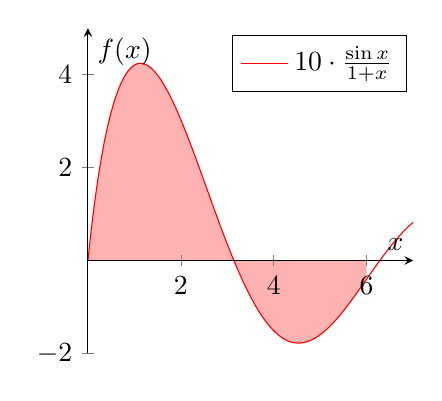
\begin{tikzpicture}[baseline]
			\begin{axis} [
				width=\textwidth / 2 - 10,
				height=\textwidth / 2 - 10,
				axis lines = center,
				axis on top=true,
				axis equal,
				ymin = -2,
				xlabel = $x$,
				ylabel = {$f(x)$},
			]
				\addplot [
					name path=f,
					domain=0:7,
					samples=100,
					color=red,
				]
				{10*sin(deg(x))/(1+x)};
				\addlegendentry{\raisebox{.5ex}{$10\cdot\frac{\sin{x}}{1+x}$}}
		
				\path[name path=axis] (axis cs:\pgfkeysvalueof{/pgfplots/xmin},0) -- (axis cs:\pgfkeysvalueof{/pgfplots/xmax},0);
				\addplot[red!30] fill between[of=f and axis, soft clip={domain=0:6}];
			\end{axis}
			\end{tikzpicture}
			~\qquad\qquad
			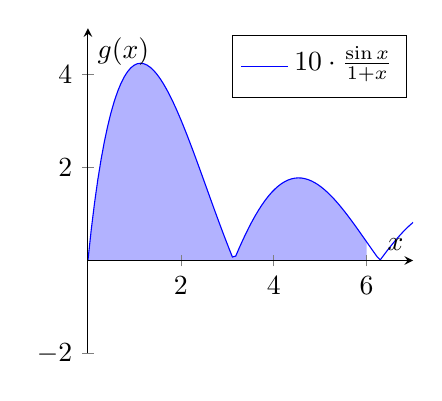
\begin{tikzpicture}[baseline]
			\begin{axis} [
				width=\textwidth / 2 - 10,
				height=\textwidth / 2 - 10,
				axis lines = center,
				axis on top=true,
				axis equal,
				ymin = -2,
				xlabel = $x$,
				ylabel = {$g(x)$},
			]
				\addplot [
					name path=g,
					domain=0:7,
					samples=100,
					color=blue,
				]
				{abs(10*sin(deg(x))/(1+x))};
				\addlegendentry{\raisebox{1ex}{$\norm{10\cdot\frac{\sin{x}}{1+x}}$}}

				\path[name path=axis] (axis cs:\pgfkeysvalueof{/pgfplots/xmin},0) -- (axis cs:\pgfkeysvalueof{/pgfplots/xmax},0);
				\addplot[blue!30] fill between[of=g and axis, soft clip={domain=0:6}];
			\end{axis}
			\end{tikzpicture}
		\end{center}
	\end{solution}
\end{exercise}

\begin{exercise}
	Perchè il \fullref{teo:cau_locale_part_1} è chiamato Teorema di Cauchy \textbf{locale}?
	\begin{solution}
		È dovuto al fatto che il teorema fornisce informazioni solo in un intorno della condizione iniziale $t_0$, non è assicurata l'esistenza di un'unica funzione risolvente in un intervallo arbitrario.
	\end{solution}
\end{exercise}

\begin{exercise}
	Confrontare l'\textbf{unicità} della soluzione di un'equazione differenziale (\fullref{teo:cau_locale_part_1}) con l'\textbf{unicità} della funzione implicita (\fullref{teo:funz_impl})
	% TODO magari la soluzione?
\end{exercise}

\subsection{Dipendenza Continua}
Nelle applicazioni fisiche, il ruolo della condizione iniziale di un problema di Cauchy è quello del valore assunto da una determinata grandezza fisica, diciamo $u_0$, misurata al tempo $t=t_0$. Poiché la misura di una grandezza fisica comporta inevitabilmente un errore di rilevazione (per quanto piccolo), è importante caratterizzare quei problemi di Cauchy tali che a fronte di piccole discrepanze $u_0 \neq v_0$ producano soluzioni $(I,u)\,(J,v)$ che differiscano ”poco” in $I\cap J$.
\begin{lemma}[Lemma di Gronwall]
	\label{lemma:gronwall}
	Dati $a,b\in \R$ con $a < b$, siano:
	\begin{itemize}
		\item $\delta_0\in \realintervalclop{0}{+\infty}$
		\item $\hspace{-0.5em}\left.\begin{array}{ll}
				k,\,\delta:\realintervalclose{a}{b}\mapsto \R \\
				k(t)\geq 0,\,\delta(t) \geq 0 \text{ funzioni continue } \forall t \in \realintervalclose{a}{b}
		\end{array} \quad\right\}$\quad cioè \quad$k,\,\delta\in\cntclass{0}(\realintervalclose{a}{b},\R^{+})$
	\end{itemize}
	con:
	$$\qquad \delta(t)\le \delta_0+\int_{a}^{t}k(\tau)\delta(\tau)\integrald{\tau}$$
	Allora
	$$\delta(t)\le\delta_0e^{\int_{a}^{t}k(\tau)\integrald{\tau}} \quad \forall t \in \realintervalclose{a}{b}$$
	Questo lemma permette di limitare una funzione che soddisfa una disuguaglianza integrale con la soluzione della corrispondente equazione. Ci si porta da una stima implicita di $\delta$ (sotto il segno di integrale) ad una stima esplicita.
	\begin{proof}
		Dividiamo in due casi
		\begin{itemize}
			\item Se $\delta_0>0$\\
				Sia $\Delta(t) = \delta_0+\int_{a}^{t}k(\tau)\delta(\tau)\integrald{\tau}$. Prendiamo ora il logaritmo di $\Delta(t)$, cioè $\ln{\bigl(\Delta(t)\bigr)}$, e deriviamolo con le regole classiche
				\begin{align*}
					\frac{d}{dt}\ln{\bigl(\Delta(t)\bigr)} &= \frac{\Delta'(t)}{\Delta(t)}\\
					&= \frac{\frac{d}{dt}\delta_0 + \frac{d}{dt}\int_{a}^{t}k(\tau)\delta(\tau)\integrald{\tau}}{\Delta(t)}
					\intertext{Il primo addendo è derivata di costante, il secondo corrisponde all'argomento dell'integrale per teorema fondamentale del calcolo integrale}
					&= \frac{0+k(t)\delta(t)}{\Delta(t)} = k(t)\frac{\delta(t)}{\Delta(t)}
					\intertext{Essendo poi, per ipotesi, $\delta(t)\leq\Delta(t)\implies\frac{\delta(t)}{\Delta(t)}\leq 1$}
					&\leq k(t)
				\end{align*}
				Integrando il primo e l'ultimo termine
				\begin{align*}
					\int_{a}^{t}\left( \frac{d}{d\tau} \ln \bigl(\Delta(\tau)\bigr) \right)\integrald{\tau} &\leq \int_{a}^{t}k(\tau)\integrald{\tau}\\
					\ln \bigl(\Delta(t)\bigr) - \ln \bigl(\Delta(a)\bigr) &\leq \int_a^t k(\tau)\integrald{\tau}
					\intertext{da definizione di $\Delta(t)$, $\Delta(a) = \delta_0$}
					\ln \bigl(\Delta(t)\bigr) &\leq \ln(\delta_0) + \int_a^t k(\tau)\integrald{\tau}
					\intertext{Passando all'esponenziale}
					e^{\ln \bigl(\Delta(t)\bigr)} &\leq e^{\bigl( \ln(\delta_0) + \int_a^t k(\tau)\integrald{\tau} \bigr)}\\
					\Delta(t) &\leq e^{\ln(\delta_0)} \cdot e^{\int_a^t k(\tau)\integrald{\tau}}\\
					\Delta(t) &\leq \delta_0e^{\int_{a}^{t}k(\tau)\integrald{\tau}}
				\end{align*}
				Da cui la tesi\\
			\item Se $\delta_0 = 0$\\
				Minoriamo, poiché $\delta_0 = 0$, con un $\epsilon > 0$
				$$\delta(t) \leq 0 + \int_{a}^{t}k(\tau)\delta(\tau)\integrald{\tau} \leq \epsilon + \int_{a}^{t}k(\tau)\delta(\tau)\integrald{\tau} \qquad \forall \epsilon > 0$$
				Essendo $\epsilon > 0$, mi trovo con una forma analoga al caso precedente, dunque
				$$\delta(t) \leq \epsilon \cdot e^{\int_{a}^{t}k(\tau)\integrald{\tau}} \qquad \forall \epsilon > 0$$
				Dovendo essere $\delta(t) \leq \epsilon \quad \forall \epsilon > 0$, posso concludere che
				$$\delta(t) \leq 0$$
				Ma, per ipotesi, $\delta(t) \geq 0 \implies \delta(t) = 0$
		\end{itemize}
	\end{proof}
\end{lemma}
\begin{exercise}
	Verificare che la funzione $\Delta$ nella dimostrazione del \fullref{lemma:gronwall} è derivabile
	\begin{solution}
		È possibile derivare la $\Delta$ perché, da \fullref{ex:funz_derivabili}, la somma di funzioni derivabili resta derivabile ed il secondo addendo è derivabile per \fullref{teo:fondament_calcolo_integ}
	\end{solution}
\end{exercise}

\begin{theorem}[Teorema di Cauchy Locale - Seconda Parte]
	\label{teo:cau_locale_part_2}
	Si considerino i seguenti problemi di Cauchy con condizione iniziale individuata nello stesso istante:
	\begin{equation}
		\label{eq:ipot_cau_part_2}
		(1)\begin{cases}x'=f(t,x)\\x(t_0)=x_0\end{cases}\qquad
		(2)\begin{cases}y'=g(t,y)\\y(t_0)=y_0\end{cases}
	\end{equation}
	con $f,g:I\times A \to \R^n$ e soddisfacenti le ipotesi di \fullref{teo:cau_locale_part_1}, cioè:
	\begin{enumerate}
		\item $t_0\in \circdot{I},\:x_0,y_0\in \circdot{A}$. Inoltre da \fullref{def:equaz_diff} e note successive: $I$ intervallo e $I\subseteq \R^n$, inoltre $A\subseteq \R^n$
		\item $f,g\in \cntclass{0}(I\times A; \R^n)$
		\item $f,g$ sono localmente Lipschitziane in $x\in A$ uniformemente rispetto a $t\in I$
	\end{enumerate}
	Allora esiste un $\delta >0$ tale che sull'intervallo $\realintervalclose{t_0-\delta}{t_0+\delta}$ sono definite una soluzione $\varphi$ di (1) ed una soluzione $\psi$ di (2). Inoltre esiste $L>0$ t.c. $\forall t\in \realintervalclose{t_0-\delta}{t_0+\delta}$ vale:
	$$\norm{\varphi(t)-\psi(t)} \le (\norm{x_0-y_0}+\delta\norm{f-g}_{\cntclass{0}})e^{L\abs{t-t_0}}$$
	dove $\norm{f-g}_{\cntclass{0}}=\sup\limits_{I\times A}\norm{f(t,x)-g(t,x)}$
	\begin{note}
		Questo significa che, con problemi diversi tra loro, se ($x_0$ e $y_0$), ($f$ e $g$) sono vicine tra loro ("a coppie"), allora sono vicine anche le soluzioni, ma per $t$ vicine.
		Pensando $t$ come tempo, cioè una delle applicazioni più classiche, questo implica che non si possano fare previsioni a lungo termine con sistemi diversi.
	\end{note}
	\begin{proof}
		Sia $f$ che $g$ soddisfano le ipotesi del \fullref{teo:cau_locale_part_1}, quindi esistono due soluzioni:
		\begin{itemize}
			\item $\varphi:\realintervalclose{t_0-\delta_f}{t_0+\delta_f}\mapsto\R$ del problema (1)
			\item $\psi:\realintervalclose{t_0-\delta_g}{t_0+\delta_g}\mapsto\R$ del problema (2)
		\end{itemize}
		Sia dunque $\delta = \min\brackets{\delta_f,\delta_g}$, da cui $J=\realintervalclose{t_0-\delta}{t_0+\delta}$ e, d'ora in poi, $t \in J$.\\
		Gli insiemi $\varphi(J)$ e $\psi(J)$ sono compatti perché per \fullref{teo:weier_generale}, essendo $J$ compatto. La loro unione è dunque un compatto, come da \fullref{ex:unione_compatti}.\\
		Utilizzando \fullref{def:equaz_volterra}, passiamo alle equazioni integrali delle \cref{eq:ipot_cau_part_2}
		\begin{equation}
			(1)\;\varphi(t)=x_0+\int_{t_0}^{t}\Bigl(f\bigl(\tau,\varphi(\tau)\bigr)\Bigr)\integrald{\tau}\qquad
			(2)\;\psi(t)=y_0+\int_{t_0}^{t}\Bigl(g\bigl(\tau,\psi(\tau)\bigr)\Bigr)\integrald{\tau}
		\end{equation}\\
		Sottraiamo ora la $(1)$ alla $(2)$ (in norma)
		\begin{align*}
			\tageq\label{eq:cau_dip_cont_diff_norm} \norm{\varphi(t)-\psi(t)} &= \norm{x_0 - y_0 + \int_{t_0}^{t}\Bigl(f\bigl(\tau,\varphi(\tau)\bigr)\Bigr)\integrald{\tau} - \int_{t_0}^{t}\Bigl(g\bigl(\tau,\psi(\tau)\bigr)\Bigr)\integrald{\tau}}\\
			&= \norm{x_0 - y_0 + \int_{t_0}^{t}\Bigl(f\bigl(\tau,\varphi(\tau)\bigr) - g\bigl(\tau,\psi(\tau)\bigr)\Bigr)\integrald{\tau}}
			\intertext{Minoriamo ora con la proprietà 3 da \fullref{def:norma}}
			&\leq \norm{x_0 - y_0} + \norm{\int_{t_0}^{t}\Bigl(f\bigl(\tau,\varphi(\tau)\bigr) - g\bigl(\tau,\psi(\tau)\bigr)\Bigr)\integrald{\tau}}
			\intertext{Minoriamo ulteriormente come da \fullref{ex:cau_loc_abs_of_norm}}
			&\leq \norm{x_0 - y_0} + \abs{\int_{t_0}^{t}\norm{f\bigl(\tau,\varphi(\tau)\bigr) - g\bigl(\tau,\psi(\tau)\bigr)}\integrald{\tau}}
			\intertext{Sommo e sottraggo nell'integrale la quantità $f\bigl(\tau,\psi(\tau)\bigr)$ (Si sarebbe potuto fare lo stesso con $g$)}
			&= \norm{x_0 - y_0} +\\
			&\qquad\abs{\int_{t_0}^{t}\norm{f\bigl(\tau,\varphi(\tau)\bigr) + f\bigl(\tau,\psi(\tau)\bigr) - f\bigl(\tau,\psi(\tau)\bigr) - g\bigl(\tau,\psi(\tau)\bigr)}\integrald{\tau}}\\
			&\leq \norm{x_0 - y_0} +\\
			&\qquad\abs{\int_{t_0}^{t}\norm{f\bigl(\tau,\varphi(\tau)\bigr) - f\bigl(\tau,\psi(\tau)\bigr)}\integrald{\tau}} + \abs{\int_{t_0}^{t}\norm{f\bigl(\tau,\psi(\tau)\bigr) - g\bigl(\tau,\psi(\tau)\bigr)}\integrald{\tau}}
			\intertext{Possiamo minorare l'argomento del secondo integrale con il $\sup\limits_{I\times A}\norm{f(t,x)-g(t,x)}$, dunque può anche essere estratto in quanto $\sup$ è costante}
			&\leq \norm{x_0 - y_0} +\\
			&\qquad\abs{\int_{t_0}^{t}\norm{f\bigl(\tau,\varphi(\tau)\bigr) - f\bigl(\tau,\psi(\tau)\bigr)}\integrald{\tau}} + \abs{\sup\limits_{I\times A}\norm{f(t,\psi(\tau))-g(t,\psi(\tau))} \int_{t_0}^{t}\integrald{\tau}}\\
			&= \norm{x_0 - y_0} +\\
			&\qquad\abs{\int_{t_0}^{t}\norm{f\bigl(\tau,\varphi(\tau)\bigr) - f\bigl(\tau,\psi(\tau)\bigr)}\integrald{\tau}} + \abs{\sup\limits_{I\times A}\norm{f(t,\psi(\tau))-g(t,\psi(\tau))} (t-t_0)}\\
			\intertext{Essendo sicuramente $t-t_0 \leq \delta$ per definizione di quest'ultimo, minoriamo ulteriormente}
			&\leq \norm{x_0 - y_0} +\\
			&\qquad\abs{\int_{t_0}^{t}\norm{f\bigl(\tau,\varphi(\tau)\bigr) - f\bigl(\tau,\psi(\tau)\bigr)}\integrald{\tau}} + \abs{\sup\limits_{I\times A}\norm{f(t,\psi(\tau))-g(t,\psi(\tau))}\delta}
			\intertext{Ricordando la \fullref{obs:dist_conv_unif}, sappiamo che $\norm{f-g}_{\cntclass{0}}=\sup\limits_{I\times A}\norm{f(t,x)-g(t,x)}$, dunque passiamo alla distanza su $\cntclass{0}$ e togliamo il valore assoluto, in quanto tutti i valori in esso contenuti sono positivi per definizione}
			&= \norm{x_0 - y_0} +\\
			&\qquad\abs{\int_{t_0}^{t}\norm{f\bigl(\tau,\varphi(\tau)\bigr) - f\bigl(\tau,\psi(\tau)\bigr)}\integrald{\tau}} + \delta\norm{f-g}_{\cntclass{0}}
			\intertext{Sia quindi $L$ costante di Lipshitz di $f$ su $J \times \bigl(\varphi(J) \cup \psi(J)\bigr)$, possiamo minorare con}
			&\leq \norm{x_0 - y_0} +\abs{\int_{t_0}^{t} L \norm{\varphi(\tau) - \psi(\tau)}\integrald{\tau}} + \delta\norm{f-g}_{\cntclass{0}}
			\intertext{Riordinando}
			&= \norm{x_0 - y_0} + \delta\norm{f-g}_{\cntclass{0}} + \abs{\int_{t_0}^{t} L \norm{\varphi(\tau) - \psi(\tau)}\integrald{\tau}}
		\end{align*}
		Applichiamo alla forma ottenuta il \fullref{lemma:gronwall}. Per ipotesi del Lemma è necessario avere $t \in \realintervalclose{a}{b}$ con $a < b$. Nell'ultimo integrale rimasto abbiamo $a = t_0$, dunque imponiamo $t \geq t_0$ e procediamo.
		\begin{note}
			Il procedimento è analogo nel caso opposto e verrà integrato sotto.
		\end{note}
		Applichamo le seguenti sostituzioni nella formula del \fullref{lemma:gronwall}:
		\begin{itemize}
			\item $k(\tau) = L$
			\item $\delta(\tau) = \norm{\varphi(\tau) - \psi(\tau)}$
			\item $\delta_0 = \norm{x_0 - y_0} + \delta\norm{f-g}_{\cntclass{0}}$ (tutti gli altri addendi)
		\end{itemize}
		Possiamo dunque minorare ulteriormente la formula precedente con
		\begin{align*}
			&\leq (\norm{x_0 - y_0} + \delta\norm{f-g}_{\cntclass{0}}) e^{\int_{t_0}^{t}L\integrald{\tau}}\\
			&= (\norm{x_0 - y_0} + \delta\norm{f-g}_{\cntclass{0}}) e^{L(t-t_0)}
		\end{align*}
		Riprendendo il primo elemento del treno di disuguaglianze \cref{eq:cau_dip_cont_diff_norm}, si ottiene infine
		\begin{align*}
			\norm{\varphi(t)-\psi(t)} &\leq (\norm{x_0 - y_0} + \delta\norm{f-g}_{\cntclass{0}}) e^{L(t-t_0)}\\
			\intertext{Inseriamo ora il valore assoluto all'esponente per tener in considerazione anche il caso in cui $t \leq t_0$}
			\norm{\varphi(t)-\psi(t)} &\leq (\norm{x_0 - y_0} + \delta\norm{f-g}_{\cntclass{0}}) e^{L\abs{t-t_0}}
		\end{align*}
	\end{proof}
\end{theorem}
\begin{note}
	Con il \fullref{teo:cau_locale_part_1} ed il \fullref{teo:cau_locale_part_2} si verifica se un Problema di Cauchy rispetta la \fullref{obs:hadamard}.
\end{note}
\begin{exercise}
	Esibire una dimostrazione dell'unicità della soluzione di un Problema di Cauchy alternativa al \fullref{teo:cau_locale_part_1} e basata sul \fullref{teo:cau_locale_part_2}.
	% TODO Soluzione
\end{exercise}
\begin{exercise}
	Enunciare il \fullref{teo:cau_locale_part_2} come risultato sulla continuità dell'\textbf{operatore di soluzione} di un Problema di Cauchy.
	% TODO Soluzione
\end{exercise}
\begin{example}
	Al variare di $p \in \R$, il Problema di Cauchy
	\begin{equation*}
		\begin{cases}
			x' = x\\
			x(0) = p
		\end{cases}
	\end{equation*}
	ha soluzione $x_p(t) = p \cdot e^t$.
	\begin{itemize}
		\item Se $t \to T \in \R$:
		$$\lim_{p \to 0}\Bigl(\lim_{t \to T} (p \cdot e^t)\Bigr) = 0 \qquad\text{e}\qquad \lim_{t \to T}\Bigl(\lim_{p \to 0} (p \cdot e^t)\Bigr) = 0$$
		I risultati coincidono, quindi c'è continuità nel parametro.
		\item Se $T \to +\infty$:
		$$\lim_{p \to 0}\Bigl(\lim_{t \to +\infty} (p \cdot e^t)\Bigr) = 0 \qquad\text{e}\qquad \lim_{t \to +\infty}\Bigl(\lim_{p \to 0} (p \cdot e^t)\Bigr) = 0$$
		I risultati son differenti, ma non solo, infatti stimando con parametri diversi mi troverei in questa situazione:
		\begin{equation}
			\label{eq:ex_cau_dip_cont_exp_dist}
			\abs{x_{p_1}(t) - x_{p_2}(t)} = \abs{p_1-p_2}e^t
		\end{equation}
		Cioè una distanza "esponenziale" tra le due soluzioni.
	\end{itemize}
	\begin{note}
		In questo esempio abbiamo $f(t,x) = x$, quindi $L = 1$, infatti $L$ stessa non appare nella \cref{eq:ex_cau_dip_cont_exp_dist}.
	\end{note}
\end{example}
\begin{example}
	Al variare di $p \in \R$, il Problema di Cauchy
	\begin{equation*}
		\begin{cases}
			x' = p\\
			x(0) = 0
		\end{cases}
	\end{equation*}
	ha soluzione $x_p(t) = p \cdot t$, cioè parametri $p$ diversi danno rette con inclinazioni diverse.
	\begin{itemize}
		\item Se $t \to T \in \R$:
		$$\lim_{p \to 0}\Bigl(\lim_{t \to T} x_p(t)\Bigr)=0 \qquad\text{e}\qquad \lim_{t \to T}\Bigl(\lim_{p \to 0} x_p(t)\Bigr)=0$$
		I risultati coincidono, quindi c'è continuità nel parametro.
		\item Se $T \to +\infty$:
		$$\lim_{p \to 0}\Bigl(\lim_{t \to +\infty} x_p(t)\Bigr)=+\infty \qquad\text{e}\qquad \lim_{t \to +\infty}\Bigl(\lim_{p \to 0} x_p(t)\Bigr)=0$$
		Essendo diversi, non c'è continuità.
	\end{itemize}
	\begin{note}
		Questo esempio evidenzia come la dipendenza continua sussista solo su intervalli finiti.
	\end{note}
\end{example}

\section{Teoria Globale}
\begin{example}[Un Problema di Cauchy senza soluzione globale]
	\label{ex:cau_glob_asint}
	Si trovi la soluzione del Problema di Cauchy
	\begin{equation}
		\begin{cases}
			x' = x^2\\
			x(0) = 1
		\end{cases}
	\end{equation}
	Essendo a variabili separabili, procediamo
	\begin{align*}
		\frac{dx}{dt} &= x^2(t)\\
		\frac{dx}{x^2(t)} &= dt\\
		\int_0^t \frac{dx}{x^2(\tau)} \integrald{\tau} &= \int_0^t \integrald{\tau}
		\intertext{Applicando al primo membro le normali regole d'integrazione delle funzioni composte otteniamo}
		-\frac{1}{x(t)} + 1 &= t\\
	\end{align*}
	Da cui si ricava $x(t) = \frac{1}{1-t}$, che è unica soluzione del Problema di Cauchy ed ha asintoto verticale in $t=1$.\\

	\begin{center}
		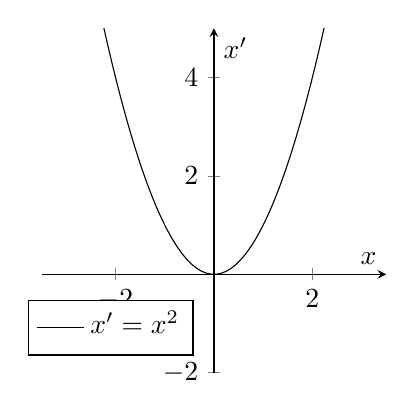
\begin{tikzpicture}[baseline]
		\begin{axis} [
		  width=\textwidth / 2 - 3,
		  height=\textwidth / 2 - 3,
		  axis lines = center,
		  axis on top=true,
		  axis equal,
		  ymin = -2,
		  ymax = 5,
		  xmin = -2,
		  xmax = 2,
		  xlabel = $x$,
		  ylabel = {$x'$},
		  legend style={at={(0.2,0.05)},anchor=south},
		]
		  \addplot [
			name path=f,
			domain=-5:5,
			samples=100,
		  ]
		  {x^2};
		  \addlegendentry{\raisebox{.5ex}{$x'=x^2$}}
		\end{axis}
		\end{tikzpicture}
		~\qquad\qquad
		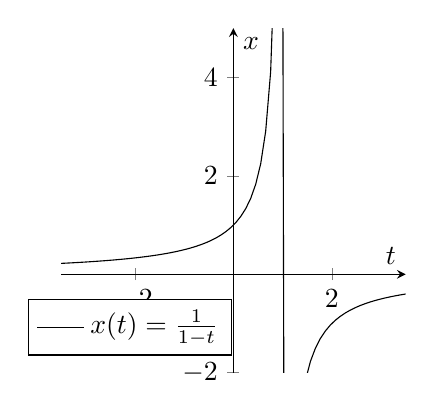
\begin{tikzpicture}[baseline]
		\begin{axis} [
		  width=\textwidth / 2 - 3,
		  height=\textwidth / 2 - 3,
		  axis lines = center,
		  axis on top=true,
		  axis equal,
		  ymin = -2,
		  ymax = 5,
		  xmin = -2,
		  xmax = 2,
		  xlabel = $t$,
		  ylabel = {$x$},
		  legend style={at={(0.2,0.05)},anchor=south},
		]
		  \addplot [
			name path=g,
			domain=-5:5,
			samples=100,
		  ]
		  {1/(1-x)};
		  \addlegendentry{\raisebox{.5ex}{$x(t) = \frac{1}{1-t}$}}
		\end{axis}
		\end{tikzpicture}
	\end{center}
	Per via dell'asintoto, nonostante la $x(t)$ abbia come dominio $\R \setminus \brackets{1}$, la soluzione del Problema di Cauchy così definito si ferma a $t=1$. Ciò perché la condizione iniziale del Problema è $t = 0 \in \realintervalopcl{-\infty}{1}$ e non avrebbe dunque senso considerare la situazione altrove. In questo intervallo di validità potrò applicare localmente il Teorema di Cauchy, ma non è possibile applicarlo globalmente.
	\begin{note}
		L'argomento di questo capitolo sarà quindi capire quando un modello sia valido globalmente.
	\end{note}
\end{example}
\begin{example}[Un Problema di Cauchy con soluzione globale]
	Il Problema di Cauchy
	\begin{equation}
		\begin{cases}
			x' = \sin(x^2)\\
			x(0) = x_0
		\end{cases}
	\end{equation}
	ammette soluzione globale $\forall x_0 \in \R$, pur non soddisfacendo alle ipotesi del \fullref{teo:cau_glob_lips}
\end{example}
\begin{example}
	Il Problema di Cauchy
	\begin{equation}
		\begin{cases}
			x' = x^2 - 1\\
			x(0) = x_0
		\end{cases}
	\end{equation}
	ammette soluzione globale per $x \in \realintervalclose{-1}{1}$, ma non per $x \in R \setminus \realintervalclose{-1}{1}$
\end{example}

\subsection{Il Caso Lipschitziano}
\begin{theorem}
	\label{teo:cau_glob_lips}
	Data la funzione $f:I \times \R^n \mapsto \R^n$, se:
	\begin{itemize}
		\item $I \subset \R$ è \textbf{intervallo compatto}
		\item $f$ è \textbf{continua} su $I \times \R^n$
		\item f è (globalmente) \textbf{Lipschitziana} in $x \in \R^n$ \textbf{uniformemente} rispetto a $t \in I$
	\end{itemize}
	Allora il Problema di Cauchy
	\begin{equation}
		\label{eq:cau_glob_thesis}
		\begin{cases}
			x' = f(x,t)\\
			x(t_0) = x_0
		\end{cases}
	\end{equation}
	ammette un'unica soluzione definita in tutto l'intervallo $I$
	\begin{proof}
		Analogamente a quanto fatto nel \fullref{teo:cau_locale_part_1}, siano:
		\begin{itemize}
			\item $X = \cntclass{0}(I,\R^n)$
			\item $T$ definita come la \cref{eq:cauch_proof_T}, cioè
				$$\funcdef{\textrm{$T$}}{\bigl(T(x)\bigr)(t)}{X}[x_0+\int_{t_0}^tf\bigl(\tau,x(\tau)\bigr)\integrald{\tau}]$$
		\end{itemize}
		I punti fissi di $T$ sono tutte e sole le soluzioni di \cref{eq:cau_glob_thesis}. Grazie al \fullref{teo:iterata_contraz}, per dimostare l'esistenza di un unico punto fisso, basta dimostrare che un'iterata di $T$ (\fullref{def:iterata}) è contrazione.\\
		Nel dettaglio andremo a dimostrare per induzione la seguente forma:
		\begin{equation}
			\norm{\bigl(T^m(x_2)\bigr)(t) - \bigl(T^m(x_1)\bigr)(t)} \leq \frac{\bigl(L \cdot \abs{t-t_0}\bigr)^m}{m!} \cdot d_X(x_2,x_1)
		\end{equation}
		Dove $L$ è costante di Lipschitzianità di $f$\\
		\begin{itemize}
			\item $m=1$: Come in dalla \cref{eq:cau_loc_verif_contraz_fine}, sappiamo che
			\begin{equation*}
				\norm{\bigl(T(x_2)\bigr)(t) - \bigl(T(x_1)\bigr)(t)} \leq \bigl(L \cdot \abs{t-t_0}\bigr) \cdot d_X(x_2,x_1)
			\end{equation*}
			\item $m>1$: Con un procedimento analogo a quello usato per giungere alla \cref{eq:cau_loc_verif_contraz_fine}, possiamo ottenere
			\begin{note}
				Le spiegazioni dei passaggi invariati possono essere viste dal \fullref{teo:cau_locale_part_1}
			\end{note}
			\begin{align*}
				&\norm{\bigl(T^{m+1}(x_2)\bigr)(t) - \bigl(T^{m+1}(x_1)\bigr)(t)} =\\
				\intertext{Per \fullref{def:equaz_volterra}}
				= &\norm{\int_{t_0}^t
				\biggl( f\Bigl(\tau,\;\bigl(T^m(x_2)\bigr)(\tau)\;\Bigr) - f\Bigl(\tau,\;\bigl(T^m(x_1)\bigr)(\tau)\;\Bigr) \biggr)
				\integrald{\tau}}\\
				\leq &\abs{\int_{t_0}^t
				\norm{ f\Bigl(\tau,\;\bigl(T^m(x_2)\bigr)(\tau)\;\Bigr) - f\Bigl(\tau,\;\bigl(T^m(x_1)\bigr)(\tau)\;\Bigr)}
				\integrald{\tau}}\\
				\leq &\abs{\int_{t_0}^t
				L \cdot \norm{\bigl(T^m(x_2)\bigr)(\tau) - \bigl(T^m(x_1)\bigr)(\tau)}
				\integrald{\tau}}
				\intertext{Grazie alla Lips. di $f$, dalla \fullref{def:loc_lips}, $\norm{\bigl(T(x_2)\bigr)(\tau) - \bigl(T(x_1)\bigr)(\tau)} \leq L \cdot d_X(x_2,x_1)$, dunque essendo $T^m$ iterata di T, si moltiplica $L$ per sé stesso $m$ volte, da cui $L^m$.\newline
				In modo analogo (penso) si ottiene $\frac{\abs{\tau-t_0}^m}{m!}$. Non lo so...} % TODO Spiegare questo passaggio
				= &\abs{\int_{t_0}^t
				L \cdot \frac{(L \cdot \abs{\tau-t_0})^m}{m!}\cdot d_X(x_2,x_1)
				\integrald{\tau}}\\
				\intertext{Riordinando i termini}
				= &\abs{\int_{t_0}^t
				\frac{L^{m+1}}{m!} \cdot d_X(x_2,x_1) \cdot \abs{\tau-t_0}^m
				\integrald{\tau}}\\
				\intertext{Essendo però i primi due fattori costanti moltiplicative non legate a $\tau$}
				= &\frac{L^{m+1}}{m!} \cdot d_X(x_2,x_1)
				\cdot \abs{\int_{t_0}^t \abs{\tau-t_0}^m \integrald{\tau}}\\
				= &\frac{L^{m+1}}{m!} \cdot d_X(x_2,x_1)
				\cdot \frac{1}{m+1} \cdot \abs{\;\left[ \abs{\tau-t_0}^{m+1} \right]_{t_0}^t\;}\\
				= &\frac{L^{m+1}}{m!} \cdot d_X(x_2,x_1)
				\cdot \frac{1}{m+1} \cdot \abs{\;\abs{t-t_0}^{m+1} - \abs{t_0-t_0}^{m+1}\;}\\
				= &\frac{L^{m+1}}{m!} \cdot d_X(x_2,x_1)
				\cdot \frac{1}{m+1} \cdot \abs{t-t_0}^{m+1}\\
				= &\frac{\bigl(L \cdot \abs{t-t_0}\bigr)^{m+1}}{m!} \cdot \frac{1}{m+1} \cdot d_X(x_2,x_1)\\
				= &\frac{\bigl(L \cdot \abs{t-t_0}\bigr)^{m+1}}{(m+1)!} \cdot d_X(x_2,x_1)\\
			\end{align*}
		\end{itemize}
		Avendo dimostrato che la minorazione vale per $m$ e per $m+1$, la dimostrazione per induzione è conclusa.
	\end{proof}
\end{theorem}

\subsection{Il Caso Sublineare}
\begin{definition}[Funzione Sublineare]
	\label{def:sublineare}
	Una funzione $f:I\times\R^n\mapsto\R^n$ con $I$ intervallo in $\R$, si dice \textbf{sublineare} se esistono due costanti $A, B:\; \forall t \in I,\;\forall x \in \R^n$ vale:
	$$\norm{f(t,x)}\leq A + B \norm{x}$$
	\begin{note}
		In sostanza una funzione è sublineare se esiste una retta tale per cui il grafico della funzione è tutto nella regione di piano delimitata da questa retta, cioè il suo grafico "non si impenna".
		\begin{center}
			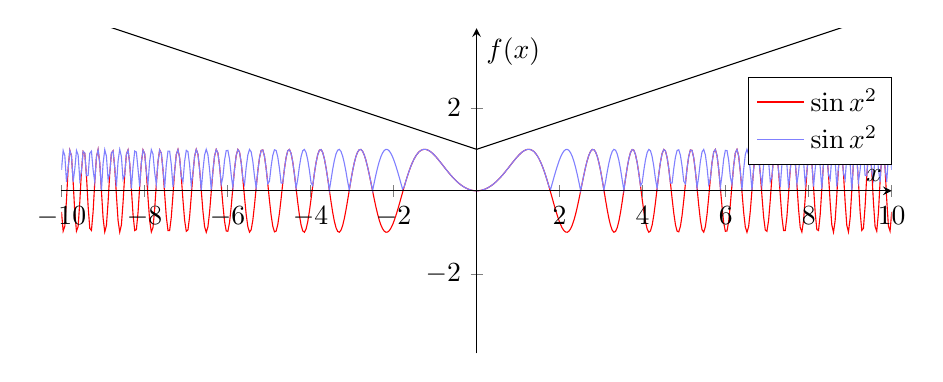
\begin{tikzpicture}
				\begin{axis} [
					width=\textwidth,
					height=\textwidth / 2 - 10,
					axis lines = center,
					axis on top=true,
					axis equal,
					ymin = -2,
					ymax = 2,
					xlabel = $x$,
					ylabel = {$f(x)$},
					legend style={at={(1,0.85)},anchor=north east},
				]
					\addplot [name path=g, domain=-10:10, samples=500, color=red] {sin(deg(x^2))};
					\addlegendentry{$\norm{\sin{x^2}}$}
					\addplot [name path=g, domain=-10:10, samples=500, color=blue!50] {abs(sin(deg(x^2)))};
					\addlegendentry{$\sin{x^2}$}
					\addplot [domain=0:10] {(1/3)*x + 1};   % The following plots are lacking a \addlegendentry, so they'll mess up with colors
					\addplot [domain=-10:0] {-(1/3)*x + 1}; % of other entries. To prevent it, any new function should be added before these
				\end{axis}
			\end{tikzpicture}
		\end{center}
	\end{note}
\end{definition}
\begin{example}
	Le seguenti funzioni sono:
	\begin{itemize}
		\begin{minipage}{0.5\linewidth}
			\item $x\cdot sin(x)$: Sublineare
			\item $sin(x^2)$: Sublineare
			\item $\frac{\arctan x^{12}}{x}$: Sublineare
		\end{minipage}
		\begin{minipage}{0.5\linewidth}
			\item $x^2\cdot sin(x)$: Non sublineare
			\item $x^2$: Non sublineare
			\item $e^x$: Non sublineare
		\end{minipage}
	\end{itemize}
\end{example}

\begin{exercise}
	Dimostrare che se una funzione $f:\R^n\mapsto\R^n$ è \textbf{(globalmente) Lipschitziana}, allora è \textbf{sublineare}
	\begin{solution}
		\begin{align*}
			&\norm{f(x)} =\\
			= &\norm{f(0) + f(x) - f(0)}\\
			\leq &\norm{f(0)} + \norm{f(x) - f(0)}
			\intertext{Per \fullref{def:lips} minoriamo}
			\leq &\norm{f(0)} + L\norm{x}
			\intertext{Ponendo ora $A = \norm{f(0)}$ e $B = L$, si ottiene}
			= &A + B\norm{x}
		\end{align*}
	\end{solution}
\end{exercise}
\begin{exercise}
	Esibire un esempio di \fullref{def:loc_lips}, ma non \textbf{sublineare}
	\begin{solution}
		$f(x) = x^2$ è loc. lips. ma non sublineare.
	\end{solution}
\end{exercise}
\begin{theorem}[Teorema di Cauchy Globale]
	\label{teo:cau_globale}
	Data la funzione $f: I \times \R^n \mapsto \R^n$, se
	\begin{enumerate}
		\item $I \subseteq \R$ è un \textbf{intervallo}
		\item $f$ è \textbf{continua} su $I\times \R^n$
		\item $f$ è \textbf{loc. lips.} in $x  \in \R^n$ \textbf{uniformemente} rispetto a $t \in I$
		\item $f$ è \textbf{sublineare}
	\end{enumerate}
	Allora il Problema di Cauchy
	\begin{equation}
		\label{eq:cau_glob_thesis_prob}
		\begin{cases}
			x' = f(t,x)\\
			x(t_0) = x_0
		\end{cases}
	\end{equation}
	Ammette un'unica soluzione definita in tutto l'intervallo $I$
	\begin{note}
		Non è necessario dimostare l'unicità in quanto la soluzione sarà localmente unica in ogni intorno di un punto e quindi si può espandere ad ogni intorno di ogni punto della soluzione.\newline
		È inoltre garantita anche la dipendenza continua, dunque è possibile scegliere un $\delta$ (dalla \fullref{teo:cau_locale_part_2}) grande a piacere
	\end{note}
	\begin{proof}
		Il \fullref{teo:cau_locale_part_1} assicura esistenda ed unicità della soluzione su un intervallo centrato nell'istante iniziale. È necessario dimostrare che la soluzione può essere estesa a tutto l'intervallo $I$ in questione. Come già parzialmente anticipato in \fullref{ex:cau_glob_asint}, questo non è possibile in due casi:
		\begin{enumerate}
			\item La soluzione ha asintoto verticale
			\item La soluzione oscilla intorno ad un punto e non continua oltre
		\end{enumerate}
		Quindi i casi in cui la soluzione non si può estendere su tutto l'intervallo sono quelli in cui non esiste il limite della soluzione. Si devono dunque evitare tali comportamenti.

		Sia $\varphi: J \mapsto \R^n$ la soluzione di \cref{eq:cau_glob_thesis_prob} e sia
		\begin{equation}
			\label{eq:cau_glob_T_M}
			T_M = \sup \brackets{\overline{t_M} \in I: \varphi\;\text{\itshape risolve \cref{eq:cau_glob_thesis_prob} su}\; \realintervalclop{t_0}{\overline{t_M}}\; }
		\end{equation}
		\begin{note}
			$T_M$ è, dunque, l'ultimo tempo fino a cui posso definire una soluzione e la $t$ utilizzata in seguito è $t \in \realintervalclop{t_0}{\overline{t_M}}$
		\end{note}
		\begin{align*}
			\varphi(t) &= x_0 + \int_{t_0}^{t} f\bigl(\tau,\varphi(\tau)\bigr)\integrald{\tau}
			\intertext{Da cui, passando alle norme e minorando per proprietà 3 della \fullref{def:norma}}
			\norm{\varphi(t)} &\leq \norm{x_0} + \norm{\int_{t_0}^{t} f\bigl(\tau,\varphi(\tau)\bigr)\integrald{\tau}}
			\intertext{Grazie all'\fullref{ex:cau_loc_abs_of_norm}}
			&\leq \norm{x_0} + \abs{\int_{t_0}^{t} \norm{f\bigl(\tau,\varphi(\tau)\bigr)}\integrald{\tau}}
			\intertext{Si può poi togliere il valore assoluto, in quanto sicuramente $t \geq t_0$ per definizione e, utilizzando la \fullref{def:sublineare}}
			&\leq \norm{x_0} + \int_{t_0}^{t} \Bigl(A + B\norm{\varphi(\tau)}\Bigr)\integrald{\tau}
			\intertext{Separando l'integrale ed essendo il primo addendo indipendente dalla variabile d'integrazione $\tau$}
			&\leq \norm{x_0} + A(t-t_0) + \int_{t_0}^{t}B\norm{\varphi(\tau)}\integrald{\tau}
			\intertext{Si minora ulteriormente, passando a $T_M$}
			&\leq \norm{x_0} + A(T_M-t_0) + \,\int_{t_0}^{t}B\norm{\varphi(\tau)}\integrald{\tau}
			\intertext{
				Dunque, applicando il \fullref{lemma:gronwall} con
				\begin{itemize}
					\item $\delta_0 = \norm{x_0} + A(T_M-t_0)$
					\item $\delta(t) = \norm{\varphi(\tau)}$
					\item $\kappa(t) = B$
					\item $a = t_0$
				\end{itemize}
			}
			\norm{\varphi(t)} &\leq \bigl(\norm{x_0} + A(T_M-t_0)\bigr)e^{\int_{t_0}^{t}B\integrald{\tau}}
			\intertext{Da cui, minorando ulteriormente con $T_M$}
			\norm{\varphi(t)} &\leq \bigl(\norm{x_0} + A(T_M-t_0)\bigr)e^{B(T_M-t_0)} \tageq\label{eq:cau_glob_gronwall}
		\end{align*}
		La $\varphi(t)$ è quindi limitata sull'intervallo $\realintervalclop{t_0}{T_M}$, dunque non è possibile abbia comportamento asintotico come quello di \fullref{ex:cau_glob_asint}. Ricordando che $\varphi(t)$ è soluzione della \cref{eq:cau_glob_thesis_prob}, otteniamo
		\begin{align*}
			\norm{\varphi'(t)} &= \norm{f\bigl(t,\varphi(t)\bigr)}\\
			&\leq \sup \limits_{t \in \realintervalclop{t_0}{T_M}} \norm{f(t,x)} \tageq\label{eq:cau_glob_dfi_sup}
		\end{align*}
		Quindi sia $\varphi(t)$ che $\varphi'(t)$ sono limitate, dunque la $\varphi$ è \textbf{uniformemente continua} su $\realintervalclop{t_0}{T_M}$, come da \fullref{prop:if_df_lim_then_unif_cont}.
		Da \fullref{prop:if_unif_cont_then_conf}, se la $\varphi(t)$ è uniformemente continua, allora è \textbf{continua}, cioò implica che $\lim \limits_{t \rightarrow T_M^-}\varphi(t) = \varphi(T_M)$.

		Essendo $\varphi(T_M) \in \R^n$, posso usare questo punto come condizione iniziale del seguente Problema di Cauchy
		\begin{equation}
			\label{eq:cau_glob_new_problem}
			\begin{cases}
				x' = f(t,x)\\
				x(T_M) = \varphi(T_M)
			\end{cases}
		\end{equation}
		Se $T_M < \sup I$, \cref{eq:cau_glob_new_problem} soddisfa le ipotesi del \fullref{teo:cau_locale_part_1}, dunque $\varphi$ può essere estesa oltre $T_M$ ad una funzione definita almeno su $\realintervalclop{t_0}{T_M+\delta}$ con $\delta > 0$ scelto opportunamente. Questa possibilità di estendere la $\varphi$ è però in contraddizione con la definizione di $T_M$ in \cref{eq:cau_glob_T_M}, dunque si deve concludere che
		$$T_M = \sup I$$
		Procedimento analogo si può svolgere per
		\begin{equation*}
			T_m = \inf \brackets{\overline{t_m} \in I: \varphi\;\text{\itshape risolve \cref{eq:cau_glob_thesis_prob} su}\; \realintervalopcl{\overline{t_m}}{t_0} }
		\end{equation*}
		I passaggi rimangono uguali fino a \cref{eq:cau_glob_gronwall} che diventa
		$$\norm{\varphi(t)} \leq \bigl(\norm{x_0} + A(T_M-t_0)\bigr)e^{B(\boldsymbol{t_0-T_m})}$$
		E, a sua volta, \cref{eq:cau_glob_dfi_sup} diventa
		\begin{align*}
			\norm{\varphi'(t)} &= \norm{f\bigl(t,\varphi(t)\bigr)}\\
			&\geq \min \limits_{t \in \realintervalopcl{T_m}{t_0}} \norm{f(t,x)}
		\end{align*}
		Dunque
		$$T_m = \inf I$$

		Grazie a come sono definiti $T_M$ e $T_m$, è stata quindi trovata una soluzione sull'intervallo $I$ che si può dire \textbf{globale} per quanto appena dimostrato.
	\end{proof}
\end{theorem}
\begin{example}
	Per ogni $x_0 \in \R$, il Problema di Cauchy
	\begin{equation*}
		\begin{cases}
			x' = x^2 \cdot \sin x\\
			x(0) = x_0
		\end{cases}
	\end{equation*}
	soddisfa le ipotesi 1., 2. e 3. del \fullref{teo:cau_globale}, ma $f(x) = x^2 \cdot \sin x$ non è né \textbf{globalmente lipschitziana}, né \textbf{sublineare} su $\R$. tuttavia, per ogni $x_0 \in \R$, questo problema ammette soluzioni globali definite su tutto $\R$
\end{example}
\begin{exercise}
	Sono date le funzioni $f_n:\R \mapsto \R$, ciascuna soddisfacente alle ipotesi del \fullref{teo:cau_globale}. Per un fissato $\overline{x}$ in $\R^n$, sia $\varphi_n$ per ogni $n \in \N$ la soluzione del Problema di Cauchy
	\begin{equation*}
		\begin{cases}
			x' = f_n(x)\\
			x(0) = \overline{x}
		\end{cases}
	\end{equation*}
	Verificare che se le $f_n$ convergono uniformemente (ricordando \fullref{def:conv_unif}), allora anche le $\varphi_n$ convergono uniformemente.
	% TODO solution
\end{exercise}


\section{Equazioni Autonome}
\begin{definition}[Equazione Autonoma]
	Un'\textbf{equazione differenziale ordinaria} si dice \textbf{autonoma} se e solo se la variabile indipendente (solitamente il tempo) non vi compare esplicitamente.
	\begin{note}
		L'assenza della variabile indipendente significa, concettualmente, che l'istante iniziale non è importante ai fini dello studio dell'equazione, ma essa dipende solo dalla lunghezza dell'intervallo.
	\end{note}
	\vspace*{-5ex}
	\begin{note}
		In fisica le equazioni differenziali autonome spesso modellizzano sistemi isolati
	\end{note}
\end{definition}
\begin{proposition}[Invarianza per Traslazione Temporale]
	Se la funzione $\varphi: \realintervalclose{a}{b} \mapsto \R^n$ risolve il Problema di Cauchy
	\begin{equation*}\begin{cases}
		x'=f(x)\\
		x(t_0) = x_0
	\end{cases}\end{equation*}
	Allora, qualunque sia $T \in \R$, la funzione $\psi: \realintervalclose{a - T}{b - T} \mapsto \R^n$ data da $\psi(t) = \varphi(t + T)$ è soluzione del Problema di Cauchy
	\begin{equation*}\begin{cases}
		x'=f(x)\\
		x(t_0 - T) = x_0
	\end{cases}\end{equation*}
	\begin{proof}
		Posta la $\psi(t)=\varphi(t+T)$
		\begin{equation*}\begin{gathered}
			\psi'(t_0)= \varphi'(t_0+T)=f(\varphi(t_0+T))=f(\psi(t_0))\\
			\psi(0)=\varphi(t_0)=x_0
		\end{gathered}\end{equation*}
	\end{proof}
\end{proposition}
\begin{proposition}
	Ogni equazione differenziale ordinaria in forma normale con secondo membro continuo è equivalente ad un'equazione autonoma.
	\begin{proof}
		\begin{equation*}
			x' = f(t,x)
			\quad\text{equivale a}\quad
			\begin{cases}
				x'=f(t,x)\\
				t'=1
			\end{cases}
		\end{equation*}
	\end{proof}
\end{proposition}
\begin{proposition}[Teorema dell'Energia Cinetica]
	\label{teo:ene_cinetica}
	Un punto materiale non vincolato $P$ di massa $m$, si muove sotto l'azione di una forza $F$ che dipende solo dalla posizione di $P$.\\
	Allora la variazione di Energia Cinetica di $P$ è uguale al lavoro compiuto su $P$ da questa forza.
	\begin{proof}
		Sia $\mathbf{x} = (x,y,z)$ la terna di coordinate di $P$. Per il Secondo Principio della Dinamica e per quanto assunto sulla forza $F$, il moto di $P$ è descritto dalla seguente equazione differenziale ordinaria vettoriale del secondo ordine
		\begin{align*}
			m \mathbf{x}'' &= F(\mathbf{x})\\
			\intertext{Dunque, moltiplicando ambo i membri}
			m \mathbf{x}'' \cdot \mathbf{x}' &= F(\mathbf{x}) \cdot \mathbf{x}'\\
			\intertext{Integrando a sinistra con la $\int{[f(x)]^nf'(x)dx}=\frac{[f(x)]^{n+1}}{n+1}+c$ posto $f(x) = \mathbf{x}'$}
			\frac{1}{2}m\frac{d}{dt}(\mathbf{x}')^2 &= F(\mathbf{x}) \cdot \mathbf{x}'\\
			\intertext{Applicando ora integrazione definita tra $0$ e $t$}
			\frac{1}{2}m\bigl(\mathbf{x}'(t)\bigr)^2 - \frac{1}{2}m\bigl(\mathbf{x}'(0)\bigr)^2 &= \int_0^t F\bigl(\mathbf{x}(\tau)\bigr) \cdot \mathbf{x}'(\tau) \integrald{\tau}\\
			\intertext{Passando alla soluzione $x$ ed alla $\xi$, traiettoria di $P$}
			\frac{1}{2}m\bigl(\mathbf{x}'(t)\bigr)^2 - \frac{1}{2}m\bigl(\mathbf{x}'(0)\bigr)^2 &= \int_{x(0)}^{x(t)} F(\xi) \integrald{\xi}
		\end{align*}
	\end{proof}
\end{proposition}
\begin{exercise}
	Estendere la dimostrazione della \fullref{teo:ene_cinetica} nel caso di $n$ punti soggetti a forze dipendenti unicamente dalle posizioni dei punti.
	% TODO solution
\end{exercise}
\begin{exercise}
	Dedurre il Principio di Conservazione dell'Energia nel caso in cui $F$ ammetta un potenziale
	% TODO solution
\end{exercise}
\begin{exercise}
	Come viene modificata la \fullref{teo:ene_cinetica} se la forza $F$ diopende anche dalla velocità $\mathbf{x}'$?
	% TODO solution
\end{exercise}
\begin{exercise}
	È possibile scrivere un'equazione differenziale ordinaria autonoma del primo ordine avente come soluzione la funzione $x(t) = \sin t$ per $t \in \realintervalclose{0}{\pi}$?\\
	E la funzione $x(t) = t^3$ per $t \in \realintervalclose{-1}{1}$?
	% TODO solution
\end{exercise}

\section{Equazioni Differenziali Lineari}
Di seguito verranno utilizzati l'identificazione ed i risultati della \fullref{sec:fun_in_C}, in particolare \fullref{ex:ext_def_in_C}
\begin{definition}
	Sia $I \subseteq \R$ un intervallo e $n \in \N$. Date le $n + 1$ funzioni $a_0,\:a_1,\:\dotsc,\:a_{n-1},\:f \quad : I \mapsto \C$, si dice \textbf{Equazione Differenziale Ordinaria Lineare di ordine} $\boldsymbol{n}$ l'equazione differenziale
	$$x^{(n)} + a_{n-1}(t) \cdot x^{(n-1)} + \dotsc + a_{1}(t) \cdot x' + a_{0}(t) \cdot x = f(t)$$
	Se $f = 0$ l'equazione si dice \textbf{Omogenea}.
\end{definition}
\proposition
sia $I$ un intervallo compatto e tale che $\circdot{I}\ne \emptyset$ siano $a_0,a_1,\ldots,a_{n-1},f\in \cntclass{0}(I;\C)$. Allora $\forall t_0\in\circdot{I}$ e $c_0,c_1,\ldots,c_{n-1}\in\C$ il problema di Cauchy 
$$ \left\{\begin{matrix}[]
x^{(n)}=-\sum\limits_{k=1}^{n-1}\left(a_k(t)x^k\right)+f(t)\\
x(t_0)=c_0\\
x(t_2)=c_1\\
\ldots\\
x^{(n-1)}(t_0)=c_{n-1}\\
\end{matrix}\right.$$
ammette soluzione unica definita su tutto l'intervallo $I$.
\begin{proof}
	Un'equazione differenziale lineare di ordine $n$ può essere trasformato in un sistema di equazioni al primo ordine.
	Introduciamo la variabile $X\in\mathbb{\cntclass{n}}$ ed il dato iniziale $C\in\mathbb{\cntclass{n}}$
	$$\left[\begin{matrix} X_1\\X_2\\\ldots\\X_{n-1}\\X_n \end{matrix}\right] = \left[\begin{matrix} x\\ x'\\\ldots\\ x^{(n-1)}\\x^{(n)} \end{matrix}\right]\quad\quad\left[\begin{matrix} C_1\\C_2\\\ldots\\C_{n-1}\\C_{n} \end{matrix}\right] = \left[\begin{matrix} c_0\\c_1\\\ldots\\ c_{n-2}\\c_{n-1} \end{matrix}\right]$$
	il problema di Cauchy per l'equazione lineare diventa:
	$$
	\left\{
	\left[\begin{matrix} X_1'\\X_2'\\\ldots\\X_{n-1}'\\X_n' \end{matrix}\right]
	=
	\left[\begin{matrix} X_2\\X_3\\\ldots\\X_{n}\\-\sum\limits_{k=1}^{n-1}\left(a_k(t)x^k\right)+f(t) \end{matrix}\right]
	\\
	X(t_0)=C
	\right.
	$$
	La funzione
	$\begin{array}{rcl} 
	F: I\times\C^n & \to & \C^n \\
	   (t,X) & \to & \left[\begin{matrix} X_2\\X_3\\\ldots\\X_{n}\\-\sum\limits_{k=1}^{n-1}\left(a_k(t)x^k\right)+f(t) \end{matrix}\right] \\ 
	\end{array}$
	è lineare in $X$ e globalmente lipschitziana in $X$ uniformemente in $t$, infatti per ogni $X,Y\in\C^n$
	$$\norm{F(t,X)-F(t,Y)}\le \sqrt{1+\left( \max\limits_k \sup\limits_I \norm{a_k} \right)^2}\cdot\norm{X-Y}$$
	Sono soddisfatte le ipotesi di Cauchy Globale allora si ha la tesi.
\end{proof}
\observation
La locuzione lineare è giustificata dalla proposizione seguente.
\proposition
Sia $I\subseteq \R$ un intervallo e $n\in\mathbb{N}$. Date le $n+1$ funzioni $a_0,a_1,\ldots,a_{n-1},f:I\to\C$,l'operatore 
$\begin{array}{rcl} 
L: \cntclass{n}(I;\C) & \to & \cntclass{0}(I;\C) \\
x & \to & x^{(n)}+\sum\limits_{k=1}^{n-1}a_k(t)x^{(k)} \\ 
\end{array}$è lineare
\begin{proof}
	La linearità di $L$ equivale a:
	$$ \begin{matrix}L(x_1+x_2)=L(x_1)+L(x_2) && \forall x_1,x_2\in \cntclass{n}(I;\C)\\L(\lambda\cdot x)=\lambda\cdot L(x) && \forall\lambda\in\C, \forall x\in \cntclass{n}(I;\C)\end{matrix} $$
	Entrambe le condizioni  seguono dalle regole di derivazione.
\end{proof}
\section{Equazioni Lineari a Coefficienti Costanti}
\definition
Dati i coefficienti $a_0,a_1,\ldots,a_{n-1},b\in\C$, si dice equazione differenziale ordinaria lineare di ordine $n$ a coefficienti costanti l'equazione differenziale
$$x^{(n)}+a_{n-1}x^{(n-1)}+\ldots+a_1 x'+a_0x=b$$
se $b=0$ l'equazione si dice omogenea. La sua Equazione caratteristica è l'equazione algebrica
$$\lambda^n+a_{n-1}\lambda^{n+1}+\ldots+a_1\lambda+a_0=0$$ 
\observation
Nella risoluzione di equazioni differenziali lineari la funzione esponenziale $t\to e^{\lambda t}$ riveste un ruolo molto particolare. Questa funzione è un autovalore dell'operatore di derivazione $D$ relativo all'autovalore, risolve infatti $\lambda$:$Dx=\lambda\cdot x$ 
\proposition
Data l'equazione
$$x^{(n)}+a_{n-1}x^{(n-1)}+\ldots+a_1 x'+a_0x=b$$
$x(t)=e^{\lambda t}$ risolve l'equazione omogenea $\iff$ $\lambda$ è soluzione dell'equazione caratteristica.\\

LEMMA:: Sia $x(t)=t\cdot e^{\lambda\cdot t}$. Allora , per ogni $n\in\mathbb{N}, n\ge 1$
$$x^{(n)}(t)=\left(\lambda^nt+n\lambda^{n-1}\right)e^{\lambda t}$$
???????????????NON L?HO CAPITA BENE.......................\\
\proposition
Data l'equazione 
$$x^{(n)}+a_{n-1}x^{(n-1)}+\ldots+a_1 x'+a_0x=b$$
$x(t)=te^{\lambda t}$ risolve l'equazione omogenea $\iff$ $\lambda$ è soluzione dell'equazione caratteristica con molteplicità almeno ??????????.

\section{Esempi}
\subsection{La Legge di Malthus}
Una popolazione, dotata di tutto il necessario per vivere e riprodursi, cresce secondo la legge di Malthus: la velocità di crescita della popolazione è proporzionale alla popolazione stessa.
$$ x'=k\cdot x$$
dove $x$ è il numero di membri della popolazione e $k$ è una costante positiva legata alla prolificità della specie in esame, generalmente calcolata come differenza tra i tassi di natalità e di mortalità.\\
Il problema di Cauchy è quindi
$$\begin{cases}
	x'=k\cdot x\\
	x(t_0)=x_0\\
\end{cases}
\qquad\text{con $x\in \R, k>0 $ e $ x_0=0$}$$

\begin{center}
	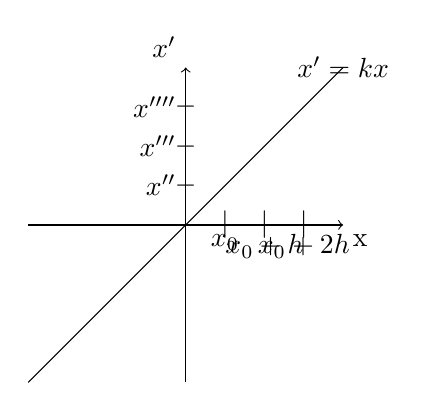
\begin{tikzpicture}[scale=1] %[x={10.0pt},y={10.0pt}]
	\pgfmathsetmacro\MAX{2}
	\draw[->] (-\MAX,0) -- (\MAX,0) node[anchor=north west] {x};
	\draw[->] (0,-\MAX) -- (0,\MAX) node[anchor=south east] {$ x'$};
	\draw[domain=-2:2,smooth,variable=\x] plot ({\x},{\x}) node {$ x'=kx$};
	\draw node at (0.5,0) {$|$};
	\draw node at (1,0) {$|$};
	\draw node at (1.5,0) {$|$};
	\draw node at (0,0.5) {$-$};
	\draw node at (0,1) {$-$};
	\draw node at (0,1.5) {$-$};
	\draw node[anchor=north] at (0.5,0) {$x_0$};
	\draw node[anchor=north] at (1,0) {$x_0+h$};
	\draw node[anchor=north] at (1.5,0) {$x_0+2h$};
	\draw node[anchor=east] at (0,0.5) {$ x'' $};
	\draw node[anchor=east] at (0,1) {$ x''' $};
	\draw node[anchor=east] at (0,1.5) {$ x''''$};
	
	\end{tikzpicture}% pic 1
	\qquad % <----------------- SPACE BETWEEN PICTURES
	\begin{tikzpicture}[scale=1] %[x={10.0pt},y={10.0pt}]
	\pgfmathsetmacro\MAX{2}
	\draw[->] (-\MAX,0) -- (\MAX,0) node[anchor=north west] {t};
	\draw[->] (0,-\MAX) -- (0,\MAX) node[anchor=south east] {x};
	\end{tikzpicture}% pic 2
\end{center}

blablabla ....\\
.......\\
Limiti di questo modello:
\begin{itemize}
	\item la variabile $x$ dovrebbe variare in $\N$, poiché una popolazione ha un numero intero di elementi.
	\item In molte specie è verosimile che il numero di nati al tempo $t$ dipenda dalla popolazione presente ad un tempo precedente $x(t-T), T>0$
	\item Supporre che una popolazione abbia per sempre a disposizione risorse sufficienti può non essere realistico
	\item Questo modello va bene quando si considerano intervalli di tempo molto lunghi.
\end{itemize}
\part{Calcolo delle Variazioni}
\part{Chapter}

\section{Preliminari}
Il calcolo delle variazioni si occupa dell'ottimizzazione di funzioni $\realfunction{F}{X}{\mathbb{R}}$, dove $X$ è un insieme di funzioni.\\
In questo capitolo varranno considerati univocamente funzionali integrali del tipo
$$\begin{array}{rcl} F: X & \to & \mathbb{R} \\
x & \to & \int_{a}^b f(t,x(t), x'(t))dt\end{array}$$
eventualmente soggetti a vincoli sui valori $x(a)$ e $x(b)$ o sul valore di un integrale del tipo $\int_a^b \varphi(x(t))dt$.\\
Dove:
$$\realfunction{f}{\realintervalclose{a}{b}\times\mathbb{R}^n\times\mathbb{R}^n}{\mathbb{R}}$$
$$X=\left\{x\in \cntclass{1}(\realintervalclose{a}{b});\mathbb{R}^n\text{ t.c.: }x(a)=x_a, x(b)=x_b \right\},\text{ con }x_a,x_b\in\mathbb{R}^n$$
\proposition
Sia $f\in \cntclass{1}(A\times\mathbb{R};\mathbb{R})$ con $a\subseteq\mathbb{R}^n$\\
Se $\begin{array}{ccc} F: \mathbb{R}\times\mathbb{R}\times A & \to & \mathbb{R} \\
x & \to & \int_{\alpha}^\beta f(x,t)dt\end{array}$
Allora:
$$ F\in \cntclass{1}$$
$$ \partial_\alpha F(\alpha,\beta,x)=-f(x,\alpha)$$
$$ \partial_\beta F(\alpha,\beta,x)=f(x,\beta)$$
$$ \nabla_x F(\alpha,\beta,x)=\int_{\alpha}^{\beta}\nabla_xf(x,t)dt$$
\definition ?????????????? R OPPURE RN\\
Sia $I\in\mathbb{R}$ un intervallo. Curva su $I$ $\mathbb{R}\rightleftharpoons$ una funzione $\gamma:I\subseteq\mathbb{R}^n$ che sia continua.
\observation
$\gamma(I)$ si chiama supporto della curva,ed 1'e certamente connesso.(una funzione continua manda intervalli connessi in connessi)
\definition
Sia $\realfunction{\gamma}{\realintervalclose{a}{b}}{\mathbb{R}}^n$ una curva, lunghezza della curva $\rightleftharpoons l(\gamma)=\sup\left\{\sum\limits_{i=1}^{N}\norm{\gamma(t_i)-\gamma(t_{i-1})}: N\in\mathbb{N}\,N>1,t_0=a,t_N=b,t_{i-1}<t_i, i=1,2,\ldots,N \right\}$ 
cioè prendo una curva e la approssimo con una spezzata, la più lunga di tutte le poligonali è la lunghezza della curva.\\
DISEGNO\\
DISEGNO\\
\definition
Una curva $\realfunction{\gamma}{\realintervalclose{a}{b}}{\mathbb{R}^n}$ si dice rettificabile $\rightleftharpoons f(\gamma)<+\infty$
\observation
$$\sum\limits_{i=1}^{N}\norm{\gamma(t_i)-\gamma(t_{i-1})} $$
per il teorema del valore medio differenziale(accrescimenti finiti)
$$\sum\limits_{i=1}^{N}\norm{ \gamma'(t_i)(t_i-t_{i-1})} =??$$
$$\int_{a}^{b}\norm{ \gamma'(t)} dt$$
\proposition
Se $\gamma\in \cntclass{1}(\realintervalclose{a}{b};\mathbb{R}^n)\Rightarrow l(\gamma)=\int_a^b\norm{\gamma'(t)}dt$
\observation
Se $\gamma$ è la traiettoria di un punto materiale,allora $\norm{\gamma}$ è la norma della velocità istantanea, e quindi $l(\gamma)$ è lo spazio che si percorre, cioè l'integrale della velocità valutato tra $t??????t_i$ due istanti di tempo entro i quali si mantiene tale velocità.
\observation
Nel caso specifico sarà:
$$ X=\left\{ x\in \cntclass{1}(\left[a,b\right];\mathbb{R}2): x(a)=A, x(b)=B \right\} $$
$$\begin{array}{ccc} 
F: X & \to & \mathbb{R} \\
x & \to & \int_{a}^b \norm{x'(t)}dt
\end{array}$$
$$\begin{array}{ccc} 
f: \left[a,b\right]\times\mathbb{R}^2\times\mathbb{R}^2 & \to & \mathbb{R} \\
(t,x, x') & \to &  \norm{x'(t)}
\end{array}$$
\section{L'Equazione di Eulero}
LEMMA:::LEMMA FONDAMENTALE DEL CALCOLO DELLE VARIAZIONI\\
Sia $f\in \cntclass{0}(\left[0,1\right];\mathbb{R})$ t.c.: $\forall v\in \cntclass{0}(\left[0,1\right];\mathbb{R})$ con $v(0)=v(1)=0$ si abbia $\int_0^1 f(x)v(x)dx=0$\\
Allora $f(x)\equiv 0\forall x\in\left[0,1\right]$ 
\begin{proof}
	\begin{center}
		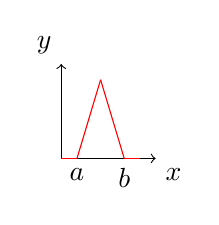
\begin{tikzpicture}[scale=1]
			\draw[->] (0,0) -- (1.2,0) node[anchor=north west] {$x$};
			\draw[->] (0,0) -- (0,1.2) node[anchor=south east] {$y$};
			\node[below] at (0.2,0) {$a$};
			\node[below] at (0.8,0) {$b$};
			\clip (0,0) rectangle (1,1);
			\draw[domain=0:0.2,smooth,red,variable=\x] plot ({\x},{0});
			\draw[domain=0.2:0.5,smooth,red,variable=\x] plot ({\x},{(1/0.3)*\x-(0.2/0.3)});
			\draw[domain=0.5:0.8,smooth,red,variable=\x] plot ({\x},{-(1/0.3)*\x+(0.8/0.3)});
			\draw[domain=0.8:1,smooth,red,variable=\x] plot ({\x},{0});
		\end{tikzpicture}
	\end{center}
	Per Assurdo, se $f\not\equiv 0$, allora $\exists\left[0,1\right]$ t.c. $f(x_0)\ne 0$.\\
	Osservo che se $x_0=0$ allora $\exists\overline{x}_0\in\left]0,1\right[$ t.c. $f(\overline{x}_0)\ne 0$.\\
	Osservo che se $x_0=1$ allora $\exists\overline{x}_0\in\left]0,1\right[$ t.c. $f(\overline{x}_0)\ne 0$\\
	Entrambe le osservazioni per la continuità di $f$, significa che se $x_0$ è un punto in cui la $f>0$ allora per la continuità della funzione anche li vicino si hanno valori maggiori di zero.\\
	Quindi si può pensare $x_0\in\left]0,1\right[$.\\
	Allora $\exists a,b\in\left]0,1\right[$ t.c. $x_0\in\left]a,b\right[ e \forall x\in\left]a,b\right[$ vale che $\abs{f(x)}\ge\abs{f(x_0)}$ sempre per la continuità di $f$.\\
	Pensiamo $f(x_0)>0$ in questo modo $\abs{f(x_0)}=f(x_0)$ e scegliamo la funzione $v(x)$ come disegnata: $v(x)=\left\{\begin{matrix}
	0&&x\le x_0-\delta\\
	\frac{x}{\delta}-\frac{x_0-\delta}{\delta}&& x_0-\delta<x<x_0\\
	1&& x=x_0\\
	-\frac{x}{\delta}+\frac{x_0+\delta}{\delta}&&x_0<x<x_0+\delta\\
	0&&x\ge x_0+\delta
	\end{matrix}\right.$POSSIBILIPLAUSIBILIERRORI\\
	Se calcoliamo
	$$\int_0^1f(x)v(x)dx=\int_a^bf(x)v(x)dx\ge\frac{1}{2}f(x_0)\int_a^bv(x)dx=\frac{1}{2}f(x_0)\frac{b-a}{2}>0$$
	Se avessi preso $f(x_0)<0$ prendo $v=-v$ e il resto segue...
\end{proof}
\observation
Questo lemma è concettualmente analogo al Teorema di Fermat nel capitolo delle derivate.
\corollary LEMMA CASO VETTORIALE.\\
Sia $f\in \cntclass{0}(\left[a,b\right];\mathbb{R}^n)$ tale che $\forall v\in \cntclass{0}(\left[a,b\right];\mathbb{R}^n)$ con $v(0)=v(1)=0$ si abbia $\int_0^1f(x)\bullet v(x)dx=0$ allora $f(x)\equiv 0$ $\forall x\in \left[0,1\right]$.
\begin{proof}
	Per questa dimostrazione si osservano componente per componente.\\
	$\forall i=1,2,\ldots,n$ scelgo $v_j(x)=\left\{\begin{matrix}0&&j\ne i\\v_i(x)&&j=i \end{matrix}\right.$\\
	A questo punto applico il lemma fondamentale alla componente $i$-esima $f_i$ di $f$.
\end{proof}
\corollary
Sia $f\in \cntclass{0}(\left[a,b\right];\mathbb{R})$ e $k\in\mathbb{N}$ tale che $\forall v\in \cntclass{k}(\left[a,b\right];\mathbb{R}^n)$ con $v(0)=v(1)=0$ si abbia $\int_0^1f(x)v(x)dx=0$ allora $f(x)\equiv 0$ $\forall x\in \left[0,1\right]$.
\begin{proof}
	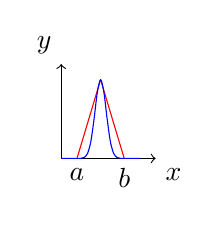
\begin{tikzpicture}[scale=1]
		\draw[->] (0,0) -- (1.2,0) node[anchor=north west] {$x$};
		\draw[->] (0,0) -- (0,1.2) node[anchor=south east] {$y$};
		\node[below] at (0.2,0) {$a$};
		\node[below] at (0.8,0) {$b$};
		\clip (0,0) rectangle (1,1);
		\draw[domain=0:0.2,smooth,red,variable=\x] plot ({\x},{0});
		\draw[domain=0.2:0.5,smooth,red,variable=\x] plot ({\x},{(1/0.3)*\x-(0.2/0.3)});
		\draw[domain=0.5:0.8,smooth,red,variable=\x] plot ({\x},{-(1/0.3)*\x+(0.8/0.3)});
		\draw[domain=0.8:1,smooth,red,variable=\x] plot ({\x},{0});
		\draw[domain=0:1,smooth,blue,variable=\x] plot ({\x},{ e^(-((\x-0.5)*10)^2) });
	\end{tikzpicture}
	\'E sempre lo stesso lemma con l'aggiunta che la funzione $v$ sia di classe $\cntclass{k}$.\\
	Se si chiama $u$ la funzione blu e $v$ la funzione rossa abbiamo:
	$$\int_0^1 f(x)u(x)dx>0$$
	Se $v$ è un po più regolare , prendiamo $v=u^(k+1)(x)$. cioè se vogliamo $v\in \cntclass{k}$ prendiamo.....\\
	LA DINMOSTRAZIONE E A ME INCOMPRENSIBILE.
\end{proof}

\theorem EQUAZIONE DI EULERO.\\
Sia $f\in \cntclass{2}\left(\left[a,b\right]\times\mathbb{R}^n\times\mathbb{R}^n;\mathbb{R}\right)$ con $a,b\in\mathbb{R}$ e $a<b$.\\
Sia $X=\left\{x\in \cntclass{2}\left(\left[a,b\right];\mathbb{R}^n\right): x(a)=A, x(b)=B\right\}$ con $A,B\in\mathbb{R}^n$.\\
Sia $\begin{array}{ccc} F: X & \to & \mathbb{R} \\
x & \to & \int_{a}^b f(t,x(t), x'(t))dt\end{array}$.\\
Se la funzione $x_\ast\in X$ è t.c. $F(x_\ast)=\max\left\{F(x):x\in X \right\}$ [o min]\\
Allora $\partial_xf(t,x_\ast(t), x_\ast'(t))-\frac{d}{dt}\partial_{ x'}f(t,x_\ast(t), x_\ast'(t))=0$.\\
Questa ultima equzione è l'equazione di Eulero-Lagrange del Funzionale $F$ o a volte detta variazione prima del funzionale $F$. è un sistema di $n$ equazioni differenziali ordinarie del secondo ordine nella funzione incognita $x_\ast$.
\begin{proof}
	 Sia $\varphi(h)=F(x_\ast+hv)$, dove $x_\ast\in X$ e $x_\ast+hv\in X$, con $h$ piccolo.\\
	 L'equazione di Eulero-Lagrange in apparenza complicata è analoga ad un equazione di analisi1 del tipo $f'=0$ oppure in analisi due a $\nabla f=0$. solo che ora sono cavoli amari.\\
	 Come si sceglie la variazione $v$ in modo che $x_\ast+hv\in X$, con $h$ piccolo.\\
	 $X$ è l'insieme delle funzioni di $\cntclass{2}$, si sa che $x_\ast\in \cntclass{2}$, una scelta opportuna di $v$ è $v\in \cntclass{2}(\left]a,b\right[;\mathbb{R}^n)$.\\
	 Inotre deve essere che $ x_\ast(a)+hv(a)=A$ e  $x_\ast(b)+hv(b)=B$ per restare dentro l'insieme $X$.
	 Quindi $v(a)=v(b)=0$.
	 $h$ è uno scalare e per ipotesi si sa che $F(x_\ast)$ è punto di massimo, quindi si conclude che $h=0$ è punto di massimo per la funzione $\varphi$.\\
	 ........ 
\end{proof}
e qui finiscono gli appunti almeno per conto mio.



% a me questo tentativo di tema esame che avevo fatto fa un po pena
% poverino è li solo soletto ed incompleto ... io lo toglierei
\chapter{Temi Esame}
\section{T.E. 2012/2013 scritto n.1}
\begin{exercise}
	Sia $f: \R^2 \to \R$ data da $f(x, y)=e^{-\abs{4\cdot arctan(x\cdot y^2)}}$
	\begin{description}
		\item[A] Nessuna delle altre affermazioni è esatta
		\item[B] $f$ ammette almeno un punto di minimo assoluto
		\item[C] $\inf_R^2f = 0$
		\item[D] $f$ ha infiniti punti di massimo
	\end{description}
	L'esponensiale è una funzione monotona crescente quindi la ricerca di massimi a minimi si sposta alla ricerca dei massimi e minimi dell'esponente.\\
	L'esponente assume sempre valori negativi. Inotre risulta essere una quantità limitata tra $[0;4\frac{\pi}{0}[$, quindi $\sup_R^2f=e^0=1$ e $\inf_R^2f=e^{-2\pi}$\\
	Sono quindi punti di massimo tutti i punti che rendono nullo l'esponente: $arctan(xy^2)=0 \implies x=0,\forall y or y=0,\forall x$ che sono i due assi. Essendo questi punti del dominio allora si può dire $\sup_R^2f=\max_R^2f=0$\\
	I punti di minimo si hanno per $\abs{arctan(xy^2)}=\frac{\pi}{2}$ quindi per $x \to \pm\infty$ or $y \to \pm\infty$ essendo questi valori al limite il valore $e^{-2\pi}$ è $inf$ per $f$\\
	La risposta vera è quindi la D.\\
\end{exercise}
\begin{exercise}
	Sia $(X,d)$ uno spazio metrico e siano $A, B$ sottoinsiemi di $X$. Quale/i delle seguenti affermazioni è/sono certamente vera/e?
	\begin{description}
		\item[1] $A\subseteq B \implies\partial A\subseteq \partial B$
		\item[2] $A\subseteq B \implies\overline{A}\subseteq\overline{B}$
	\end{description}
	\begin{description}
		\item[A] Entrambe
		\item[B] Solo la seconda
		\item[C] Nessuna delle affermazioni è esatta
		\item[D] Solo la prima
	\end{description}
	La prima affermazione è certamente falsa poiché se scelto come spazio metrico $R^2$ con distanza quella eclidea. Scelgo $A=B((0,0),2), A=B((0,0),1)$ allora si ha che $\partial A = \{(x,y)\in \R^2:d((x,y),(0,0))=2\}$ e $\partial B = \{(x,y)\in \R^2:d((x,y),(0,0))=1\}$ e questi due insiemi sono disgiunti.\\
	la seconda è vera ma devo pensarci un po...\\
\end{exercise}




\backmatter
% bibliography, glossary and index would go here.

\end{document}